%%==========================================================================
%% This is the very first version of a Streetwise LaTeX template. By
%% chosing the document class, it is easily convertible to a two-column IEEE
%% paper format, provided any conflicting packages and (new)commmands are
%% removed.
%%
%% Erwin de Gelder, January 6, 2018
%%==========================================================================

%%==========================================================================
%% Title:
%% Author(s):
%% To be published in:
%% Date of submission:
%% Date of submission R1:
%% Date of submission R2:
%% Date of final submission:
%%==========================================================================


%% Generic
\documentclass[10pt,final,a4paper,oneside,onecolumn]{article}

%% IEEE
%% Document class options: replace "draftcls" by "final" for final document.
%% All other options may just as well be omitted because they are the default values.
%\documentclass[10pt,final,journal,letterpaper,twoside,twocolumn]{IEEEtran}


%%==========================================================================
%% Document automation
%%==========================================================================

\def\reptitle{Hyperparameter selection for scenario generation}
\def\repauthor{Erwin de Gelder, etc.}


%%==========================================================================
%% Packages
%%==========================================================================

\usepackage[a4paper,left=3.5cm,right=3.5cm,top=3cm,bottom=3cm]{geometry} %% change page layout; remove for IEEE paper format
\usepackage[T1]{fontenc}                        %% output font encoding for international characters (e.g., accented)
\usepackage[cmex10]{amsmath}                    %% math typesetting; consider using the [cmex10] option
\usepackage{amssymb}                            %% special (symbol) fonts for math typesetting
\usepackage{amsthm}                             %% theorem styles
\usepackage{dsfont}                             %% double stroke roman fonts: the real numbers R: $\mathds{R}$
\usepackage{mathrsfs}                           %% formal script fonts: the Laplace transform L: $\mathscr{L}$
\usepackage[pdftex]{graphicx}                   %% graphics control; use dvips for TeXify; use pdftex for PDFTeXify
\usepackage{array}                              %% array functionality (array, tabular)
\usepackage{upgreek}                            %% upright Greek letters; add the prefix 'up', e.g. \upphi
\usepackage[noadjust]{cite}                     %% citations; noadjust removes leading spaces
%\usepackage[round]{natbib}                     %% Author-year citations (remove package cite)
\usepackage{stfloats}                           %% improved handling of floats
\usepackage{multirow}                           %% cells spanning multiple rows in tables
%\usepackage{subfigure}                         %% subfigures and corresponding captions (for use with IEEEconf.cls)
\usepackage{subfig}                             %% subfigures (IEEEtran.cls: set caption=false)
\usepackage{fancyhdr}                           %% page headers and footers
\usepackage[official,left]{eurosym}             %% the euro symbol; command: \euro
\usepackage{appendix}                           %% appendix layout
\usepackage{xspace}                             %% add space after macro depending on context
\usepackage{verbatim}                           %% provides the comment environment
\usepackage[dutch,USenglish]{babel}             %% language support
\usepackage{wrapfig}                            %% wrapping text around figures
\usepackage{longtable}                          %% tables spanning multiple pages
%\usepackage[utf8]{inputenc}
\usepackage{pgfplots}                           %% support for TikZ figures (Matlab)
\usepackage[breaklinks=true,hidelinks,          %% implement hyperlinks (dvips yields minor problems with breaklinks;
            bookmarksnumbered=true]{hyperref}   %% IEEEtran: set bookmarks=false)
%\usepackage[hyphenbreaks]{breakurl}            %% allow line breaks in URLs (don't use with PDFTeX)
\usepackage{lmodern} 
\usepackage{etoolbox}							%% Needed for apptocmd later

%%==========================================================================
%% Fancy headers and footers
%%==========================================================================

\pagestyle{fancy}                                       %% set page style
\fancyhf{}                                              %% clear all header & footer fields
\fancyhead[L]{
\includegraphics[width=15mm]{Streetwise}} %% define headers (LE: left field/even pages, etc.)
\fancyhead[R]{\small\emph{\reptitle}}                   %% similar
\fancyfoot[C]{\thepage}                                 %% define footer
\setlength{\headheight}{18pt}                           %% increase head height to accommodate an oversized picture in the header
\renewcommand*{\headrulewidth}{0.25pt}                  %% header line width
\renewcommand*{\footrulewidth}{0pt}                     %% footer line width
%% Redefine the default "plain" page style (automatically activated by \maketitle, \section, ...)
\fancypagestyle{plain}{\fancyhf{}
                       \fancyhead[C]{
\includegraphics[width=30mm]{Streetwise}}
                       \renewcommand{\headrulewidth}{0pt}
                       \renewcommand{\footrulewidth}{0pt}
                       \setlength{\headheight}{36pt}}


%%==========================================================================
%% TikZ figures
%%==========================================================================

\newlength\figurewidth
\setlength\figurewidth{0.35\textwidth}              %% set figure height
\newlength\figureheight
\setlength\figureheight{0.3\textwidth}              %% set figure width
\pgfplotsset{every axis/.append style={
    scaled y ticks=false,
    scaled x ticks=false,
    y tick label style={/pgf/number format/fixed},
    x tick label style={/pgf/number format/fixed},
    legend style={font=\small}},
    compat=1.9}                                     %% PGFPlots package options
\usetikzlibrary{arrows}                             %% plot arrows
\usetikzlibrary{external}                           %% Create pdf figures from TikZ. Use PDFTeXify ...
\tikzexternalize[prefix=./tikz/]                    %% ... with --tex-option=--shell-escape switch.
%\tikzset{external/force remake}                    %% force pdf figure update


%%==========================================================================
%% User-defined commands
%%==========================================================================

\newcommand*{\mat}[1]{\mathbf{#1}}                              %% matrix/vector notation
\newcommand*{\matsym}[1]{\boldsymbol{#1}}                       %% matrix/vector notation for Greek letters
\newcommand*{\T}{^{\scriptscriptstyle\mathsf{T}}}               %% transpose operator
\newcommand*{\Hr}{^{\scriptscriptstyle\mathsf{H}}}              %% conjugate transpose operator
\newcommand*{\ud}{\mathrm{\,d}}                                 %% differential operator (upright d)
\newcommand*{\defeq}{\mathrel{\mathop:}=}                       %% definition sign :=
\newcommand*{\eqdef}{=\mathrel{\mathop:}}                       %% definition sign =:
\newcommand*{\ip}[2]{\left\langle#1\,{,}\,#2\right\rangle}      %% inner product
\newcommand*{\real}[1]{\mathrm{Re}(#1)}                         %% real part
\newcommand*{\imag}[1]{\mathrm{Im}(#1)}                         %% imaginary part
\newcommand*{\lsup}[1]{{}^{#1}\!}                               %% left superscript
\newcommand*{\hi}[1]{$^\text{#1}$}                              %% superscript in normal text
\newcommand*{\lo}[1]{$_\text{#1}$}                              %% subscript in normal text
\newcommand*{\w}[1]{\mathrm{#1}}                                %% multiple character super-/subscript in math mode
\newcommand*{\Ln}{{\ensuremath{\mathcal{L}}}\xspace}            %% L norm
\newcommand*{\Lone}{{\ensuremath{\mathcal{L}_1}}\xspace}        %% L_1 norm
\newcommand*{\Ltwo}{{\ensuremath{\mathcal{L}_2}}\xspace}        %% L_2 norm
\newcommand*{\Linf}{{\ensuremath{\mathcal{L}_\infty}}\xspace}   %% L_inf norm
\newcommand*{\Lp}{{\ensuremath{\mathcal{L}_p}}\xspace}          %% L_p norm
\newcommand*{\Htwo}{{\ensuremath{\mathcal{H}_2}}\xspace}        %% H_2 norm
\newcommand*{\Hinf}{{\ensuremath{\mathcal{H}_\infty}}\xspace}   %% H_inf norm
\newcommand*{\Hp}{{\ensuremath{\mathcal{H}_p}}\xspace}          %% H_p norm
\newcommand*{\capskip}{\vspace{-12pt}}                          %% caption skip for figures with subfloats
\newcommand*{\etal}{et al.}                                     %% may be required for Natbib bibliography styles
\renewcommand*{\qedsymbol}{$\blacksquare$}                      %% redefine the end-of-proof symbol
\renewcommand*{\labelitemi}{$\bullet$}                          %% first level item list bullet
\renewcommand*{\labelitemii}{$-$}                               %% second level item list bullet
%\renewcommand*{\theenumi}{\textit{\roman{enumi}}}               %% first level enumerator
\renewcommand*{\labelenumi}{\theenumi.}
\renewcommand*{\theenumii}{\textit{\alph{enumii}}}              %% second level enumerator
\renewcommand*{\labelenumii}{\theenumii.}
\DeclareMathOperator{\tr}{tr}                                   %% trace of a matrix
\DeclareMathOperator{\sgn}{sgn}                                 %% signum function
\DeclareMathOperator{\atan}{atan}                               %% arc tangent


%%==========================================================================
%% User-defined environments
%%==========================================================================

\theoremstyle{plain}\newtheorem{definition}{Definition}[section]    %% definition
                    \newtheorem{theorem}{Theorem}[section]          %% theorem
                    \newtheorem{lemma}[theorem]{Lemma}              %% lemma
                    \newtheorem{corollary}[theorem]{Corollary}      %% corollary
                    \newtheorem{assumption}{Assumption}[section]    %% assumption
                    \newtheorem{condition}{Condition}[section]      %% condition
\theoremstyle{definition}\newtheorem{example}{Example}[section]     %% examples
\theoremstyle{remark}\newtheorem{remarkenv}{Remark}[section]        %% remarks
\newenvironment{remark}{\begin{remarkenv}}%
                       {\hfill$\blacklozenge$\end{remarkenv}}       %% end remark with a lozenge
\newenvironment{reviewer}{\itshape}{\upshape}                       %% environment for reviewer's comments


%%==========================================================================
%% Miscellaneous
%%==========================================================================

\graphicspath{{./../}{./figures/}{./more_figures/}} %% (graphicx) directory path for figures
%\setlength{\parindent}{0pt}                        %% no paragraph indentation
%\setlength{\parskip}{2ex}                          %% create empty line between paragraphs
%\interdisplaylinepenalty=2500                      %% (amsmath) allow for page breaks within multiline equations
%\numberwithin{equation}{section}                   %% (amsmath) include section number in equation numbering
%\numberwithin{figure}{section}                     %% (amsmath) include section number in figure numbering
%\numberwithin{table}{section}                      %% (amsmath) include section number in table numbering
\addtolength{\arraycolsep}{-0.5mm}                  %% squeeze matrix columns a little
\fnbelowfloat                                       %% (stfloats) put footnote below a float at the page bottom
\urlstyle{same}                                     %% (hyperref) use current font for URLs
\hypersetup{pdftitle={\reptitle},
            pdfauthor={\repauthor}}                 %% (hyperref) pdf properties title and author
%\raggedbottom                                      %% don't add inter-paragraph spacing to achieve \textheight
%\setlength\subfigcapskip{-3pt}                     %% (subfigure) distance between subfloat and subcaption
%\setlength\subfigbottomskip{-3pt}                  %% (subfigure) distance between subcaption and caption
%\renewcommand*{\subcapsize}{\small}                %% (subfigure) subcaption font size
\renewcommand*{\thesubfigure}{(\alph{subfigure})}   %% (subfig) implement 1(a) instead of 1a ...as subfigure reference
\captionsetup[subfloat]{labelformat=simple}        %% ... as subfigure reference
%\captionsetup[subfloat]{
%    farskip=0pt,
%    nearskip=8pt,
%    captionskip=1.5pt,
%    labelfont={small,bf},
%    textfont=small}                                %% (subfig) subfloat caption format
%\captionsetup[figure]{
%    labelfont={small,bf},
%    textfont=small}                                %% (subfig/caption) figure caption format
%\captionsetup[table]{
%    aboveskip=2pt,
%    labelfont={small,bf},
%    textfont={small,sc}}                           %% (subfig/caption) table caption format
\bibliographystyle{IEEEtran}                        %% (BibTeX) references style, e.g., IEEEtran, plainnat, abbrvnat, unsrtnat, or thesisnat
\apptocmd{\thebibliography}{\raggedright}{}{}		%% Suppress badness warnings in bibliography


%%==========================================================================
%% Begin document
%%==========================================================================

\begin{document}

\selectlanguage{USenglish}

\title{\textbf{\reptitle}}
\author{\repauthor}
\date{\today}
\maketitle

\tableofcontents

\newpage

\section{Introduction}

For the generation of test scenarios for the performance assessment of Automated Vehicles (AVs), it is important to generate realistic trajectories of vehicles. Real-life data could be used to generate realistic trajectories \cite{deGelder2017assessment}. In Figure~\ref{fig:velocity example}a, an example of a velocity profile from real-life driving data is shown. The recorded trajectories from the real-life data need to be parametrized, such that probability density functions (PDFs) can be estimated. From these estimation PDFs, new parameters can be generated. These generated parameters are then used to generate a trajectory. 

\begin{figure}[b]
	\centering
	\setlength\figureheight{150pt}
	\setlength\figurewidth{0.49\linewidth}
	\subfloat[Original]{% This file was created by matplotlib2tikz v0.6.14.
\begin{tikzpicture}

\definecolor{color0}{rgb}{0.12156862745098,0.466666666666667,0.705882352941177}

\begin{axis}[
xlabel={Time [s]},
ylabel={Velocity [km/h]},
xmin=-0.293991395216091, xmax=6.17381929953791,
ymin=7.506, ymax=35.622,
width=\figurewidth,
height=\figureheight,
tick align=outside,
tick pos=left,
xmajorgrids,
x grid style={white!69.019607843137251!black},
ymajorgrids,
y grid style={white!69.019607843137251!black}
]
\addplot [semithick, color0, forget plot]
table {%
0 33.984
0.0399989420671147 34.344
0.0799978841342437 34.02
0.119996826201358 34.056
0.159996163019557 34.02
0.199995105086685 34.128
0.2399940471538 34.056
0.279992989220929 34.02
0.319991931288044 33.84
0.359990873355173 33.876
0.399989815422288 33.768
0.439988757489417 33.588
0.479987699556531 33.408
0.51998664162366 33.264
0.559985583690775 33.012
0.599997157792259 32.832
0.679995041926503 32.544
0.719993983993632 32.292
0.759992926060747 32.22
0.799991868127876 31.86
0.83999081019499 31.644
0.879989752262119 31.536
0.919988694329234 31.248
0.959987636396363 30.852
0.999986578463478 30.672
1.03998552053061 30.492
1.07998446259772 30.132
1.11998340466485 29.952
1.15998234673197 29.592
1.19998128879909 29.304
1.23998023086621 29.088
1.27997917293334 28.836
1.31997811500045 28.584
1.35997705706758 28.296
1.3999759991347 27.864
1.43997494120183 27.72
1.47997427802002 27.324
1.51997322008714 27.036
1.55997216215427 26.784
1.59997110422138 26.46
1.63997004628851 26.136
1.67996898835563 25.92
1.71995529838838 25.632
1.75995424045551 25.2
1.79995318252263 25.092
1.83995172983867 24.732
1.87995106665687 24.372
1.919950008724 24.084
1.95994895079112 23.832
1.99994789285824 23.472
2.03994683492536 23.184
2.07994577699249 22.896
2.1199447190596 22.536
2.15994366112673 22.356
2.19994260319385 22.068
2.23994154526098 21.6
2.31993942939522 21.204
2.35993837146233 20.808
2.39993731352946 20.592
2.43993625559658 20.196
2.47993519766371 19.944
2.51993413973082 19.8
2.55993308179795 19.512
2.59993202386507 19.224
2.63993096593219 19.044
2.67992990799931 18.756
2.71992885006644 18.468
2.75992779213355 18.324
2.79992673420068 18.036
2.8399256762678 17.784
2.87992461833493 17.712
2.91992356040204 17.496
2.95992250246917 17.28
3.03992038660341 17.1
3.07991932867053 16.992
3.11991827073766 17.028
3.15991721280477 16.848
3.23990364915787 16.776
3.279902591225 16.668
3.31990153329211 16.596
3.35990047535924 16.524
3.39989941742635 16.38
3.4798973015606 16.344
3.51989624362773 16.2
3.59989412776197 16.092
3.63989306982909 16.02
3.67989201189621 15.984
3.71989095396333 15.948
3.75988989603046 15.804
3.8398877801647 15.624
3.87988672223183 15.48
3.95988460636607 15.372
3.99988354843319 15.156
4.03988249050032 15.192
4.07988143256743 14.976
4.11988037463456 14.832
4.15987931670168 14.652
4.19987825876881 14.544
4.23987720083592 14.436
4.27987614290305 14.4
4.31987508497016 14.22
4.35987402703729 14.04
4.39987296910441 14.004
4.43987191117154 13.788
4.47987085323865 13.644
4.51986979530578 13.5
4.55986873737289 13.32
4.59986767944002 13.176
4.63986662150714 13.068
4.67986556357427 12.996
4.71986450564138 12.744
4.75986344770851 12.636
4.79986238977563 12.42
4.83986133184276 12.276
4.87986027390987 12.204
4.919859215977 12.096
4.95985815804411 11.988
4.99985710011124 11.808
5.03985012091225 11.592
5.07984906297938 11.52
5.11984800504649 11.412
5.15984694711362 11.196
5.19984588918074 11.124
5.23984483124786 10.944
5.27984377331498 10.764
5.31984271538211 10.692
5.35984165744922 10.548
5.39984059951635 10.332
5.43983954158347 10.26
5.4798384836506 10.044
5.51983742571771 9.864
5.55983636778484 9.792
5.59983530985195 9.612
5.63983425191908 9.468
5.6798331939862 9.36
5.71983213605333 9.216
5.75983107812044 9.072
5.79983002018757 9
5.83982896225469 8.82
5.87982790432181 8.784
};
\end{axis}

\end{tikzpicture}}
	\subfloat[Normalized]{% This file was created by matplotlib2tikz v0.6.14.
\begin{tikzpicture}

\definecolor{color0}{rgb}{0.12156862745098,0.466666666666667,0.705882352941177}

\begin{axis}[
xlabel={Normalized time},
ylabel={Normalized velocity},
xmin=-0.05, xmax=1.05,
ymin=-0.05, ymax=1.05,
width=200pt,
height=130pt,
tick align=outside,
tick pos=left,
xmajorgrids,
x grid style={white!69.019607843137251!black},
ymajorgrids,
y grid style={white!69.019607843137251!black}
]
\addplot [semithick, color0, forget plot]
table {%
0 0.985915492957746
0.00680274027029168 1
0.0136054805405858 0.987323943661972
0.0204082208108775 0.988732394366197
0.0272110282176721 0.987323943661972
0.0340137684879662 0.991549295774648
0.0408165087582578 0.988732394366197
0.0476192490285519 0.987323943661972
0.0544219892988436 0.980281690140845
0.0612247295691377 0.98169014084507
0.0680274698394294 0.977464788732394
0.0748302101097235 0.970422535211268
0.0816329503800152 0.963380281690141
0.0884356906503093 0.957746478873239
0.095238430920601 0.947887323943662
0.102043319558936 0.940845070422535
0.115648800099522 0.929577464788732
0.122451540369816 0.919718309859155
0.129254280640107 0.916901408450704
0.136057020910402 0.902816901408451
0.142859761180693 0.894366197183099
0.149662501450987 0.890140845070422
0.156465241721279 0.87887323943662
0.163267981991573 0.863380281690141
0.170070722261865 0.856338028169014
0.176873462532159 0.849295774647887
0.183676202802451 0.835211267605634
0.190478943072745 0.828169014084507
0.197281683343036 0.814084507042254
0.20408442361333 0.802816901408451
0.210887163883622 0.794366197183099
0.217689904153916 0.784507042253521
0.224492644424208 0.774647887323944
0.231295384694502 0.763380281690141
0.238098124964794 0.746478873239437
0.244900865235088 0.740845070422535
0.251703672641882 0.725352112676056
0.258506412912174 0.714084507042253
0.265309153182468 0.704225352112676
0.27211189345276 0.691549295774648
0.278914633723054 0.67887323943662
0.285717373993346 0.670422535211267
0.292517965895596 0.659154929577465
0.299320706165891 0.64225352112676
0.306123446436182 0.638028169014084
0.312926119569973 0.623943661971831
0.319728926976768 0.609859154929577
0.326531667247062 0.598591549295775
0.333334407517354 0.588732394366197
0.340137147787648 0.574647887323944
0.34693988805794 0.563380281690141
0.353742628328234 0.552112676056338
0.360545368598525 0.538028169014084
0.367348108868819 0.530985915492958
0.374150849139111 0.519718309859155
0.380953589409405 0.501408450704225
0.394559069949991 0.485915492957746
0.401361810220283 0.470422535211268
0.408164550490577 0.461971830985915
0.414967290760868 0.446478873239437
0.421770031031163 0.436619718309859
0.428572771301454 0.430985915492958
0.435375511571748 0.419718309859155
0.44217825184204 0.408450704225352
0.448980992112334 0.401408450704225
0.455783732382626 0.390140845070422
0.46258647265292 0.37887323943662
0.469389212923212 0.373239436619718
0.476191953193506 0.361971830985915
0.482994693463797 0.352112676056338
0.489797433734091 0.349295774647887
0.496600174004383 0.340845070422535
0.503402914274677 0.332394366197183
0.517008394815263 0.325352112676056
0.523811135085555 0.32112676056338
0.530613875355849 0.322535211267606
0.53741661562614 0.315492957746479
0.551020149208187 0.312676056338028
0.557822889478481 0.308450704225352
0.564625629748773 0.305633802816901
0.571428370019067 0.302816901408451
0.578231110289358 0.297183098591549
0.591836590829944 0.295774647887324
0.598639331100238 0.290140845070422
0.612244811640824 0.285915492957746
0.619047551911116 0.283098591549296
0.62585029218141 0.28169014084507
0.632653032451702 0.280281690140845
0.639455772721996 0.274647887323944
0.653061253262581 0.267605633802817
0.659863993532876 0.261971830985915
0.673469474073461 0.257746478873239
0.680272214343753 0.249295774647887
0.687074954614047 0.250704225352113
0.693877694884339 0.242253521126761
0.700680435154633 0.236619718309859
0.707483175424925 0.229577464788732
0.714285915695219 0.225352112676056
0.72108865596551 0.22112676056338
0.727891396235804 0.219718309859155
0.734694136506096 0.212676056338028
0.74149687677639 0.205633802816901
0.748299617046682 0.204225352112676
0.755102357316976 0.195774647887324
0.761905097587268 0.190140845070423
0.768707837857562 0.184507042253521
0.775510578127853 0.177464788732394
0.782313318398147 0.171830985915493
0.789116058668439 0.167605633802817
0.795918798938733 0.164788732394366
0.802721539209025 0.154929577464789
0.809524279479319 0.150704225352113
0.816327019749611 0.142253521126761
0.823129760019905 0.136619718309859
0.829932500290196 0.133802816901408
0.836735240560491 0.129577464788732
0.843537980830782 0.125352112676056
0.850340721101076 0.11830985915493
0.857142454323848 0.109859154929577
0.863945194594142 0.107042253521127
0.870747934864434 0.102816901408451
0.877550675134728 0.0943661971830986
0.88435341540502 0.0915492957746479
0.891156155675314 0.0845070422535211
0.897958895945606 0.0774647887323944
0.9047616362159 0.0746478873239437
0.911564376486191 0.0690140845070423
0.918367116756485 0.0605633802816902
0.925169857026777 0.0577464788732394
0.931972597297071 0.0492957746478873
0.938775337567363 0.0422535211267606
0.945578077837657 0.0394366197183099
0.952380818107949 0.0323943661971831
0.959183558378243 0.0267605633802817
0.965986298648534 0.0225352112676056
0.972789038918828 0.0169014084507042
0.97959177918912 0.0112676056338028
0.986394519459414 0.00845070422535212
0.993197259729706 0.00140845070422538
1 0
};
\end{axis}

\end{tikzpicture}}
	\caption{Example of a velocity profile from real-life driving data.}
	\label{fig:velocity example}
\end{figure}

In the process of going from real-life driving data to the generation of new trajectories, there are many choices to be made. For example, how should the parametrization be performed? How should the PDFs be estimated? To answer these questions, it would be useful to have a measure that objectively measures how good these choices are. This document describes such a method.

In the remainder of this document, we are dealing with the normalized velocity profiles, such that the profile starts at $(0,1)$ and ends at $(1,0)$. Figure~\ref{fig:velocity example}b shows the normalized profile of the original velocity profile shown in Figure~\ref{fig:velocity example}a.

\section{Method}
\label{sec:method}

\subsection{Alternative for likelihood}
\label{sec:method alternative likelihood}

When tuning the hyper-parameters for a specific model, often the data is split into a training and a test set, such that the training set is used to fit a model, while the test set is used to ``measure'' how good the fitted model fits the test data. One approach for measuring how good the model fits the test data, is by determining the likelihood that the test data would have been generated by the model. The higher the likelihood, the better the model fits to the test data. Let $y_i$ with $i \in {1, \ldots, n}$ denote the test data. When assuming $y_i$ and $y_j$ to be independent from each other for $i \neq j$, the likelihood $P$ that the test data comes from a PDF $p(Z)$ is
\begin{equation} \label{eq:likelihood}
	P = \prod_{i=1}^n p(y_i).
\end{equation}

The probability $p(y_i)$ can be rewritten as follows:
\begin{equation} \label{eq:probability with dirac}
	p(y_i) = \int \delta(z-y_i) p(z) dz,
\end{equation}
where $\delta(\cdot)$ denotes the Dirac function. When substituting Eq.~\eqref{eq:probability with dirac} into Eq.~\eqref{eq:likelihood}, we obtain
\begin{equation} \label{eq:likelihood in complicated way}
	P = \prod_{i=1}^n \int \delta(z - y_i) p(z) dz.
\end{equation}

A problem arises when using the likelihood of Eq.~\eqref{eq:likelihood} for generating the normalized velocity profiles. In this case, $y_i$ refers to the test profiles, for which an example is shown in Figure~\ref{fig:velocity example}b. Note that, therefore, $y_i$ depends on the normalized time $t \in [0,1]$, so we can write it as $y_i(t)$ to emphasize the dependence on $t$. Furthermore, $z$ refers to the (generated) parameters of the velocity profile. Hence, $y_i(t)$ cannot be subtracted from $z$. Even if we consider the profile generated with parameters $z$, denoted by $g_z(t)$, the use of the likelihood of Eq.~\eqref{eq:likelihood}, or similar Eq.~\eqref{eq:likelihood in complicated way}, is problematic, because the generated profile will never be exactly equal to a test profile, due to the parametrization. Therefore, an alternative approach is required.

Now, let us define a ``score'' which is very similar to Eq.~\eqref{eq:likelihood in complicated way}, but with a so-called similarity measure $f(z,y)$:
\begin{equation} \label{eq:score}
	J = \prod_{i=1}^n \int f(z,y_i)p(z)dz.
\end{equation}
Note that Eq.~\eqref{eq:score} can be estimated using a Monte Carlo approach, i.e.
\begin{equation} \label{eq:score monte carlo}
	J \approx \prod_{i=1}^n \frac{1}{N} \sum_{j=1}^N f(z_j, y_i), \quad z_j \sim p(Z)
\end{equation}
for large $N$.

\subsection{Similarity measure}
\label{sec:method similarity function}

The success of the score function of Eq.~\eqref{eq:score} depends on the similarity $f(z,y)$. The similarity measure should satisfy the following requirements:
\begin{itemize}
	\item $f(z,y) \geq 0, \forall z, y$
	\item $f(z,y) \approx 0$ when the generated profile with parameters $z$ looks completely different from the profile $y$.
	\item $f(z,y) \gg 0$ when the generated profile with parameters $z$ looks very similar to the profile $y$.
\end{itemize}

One approach is to define a distance function $d(g_z(t), y(t)) \geq 0$ which returns a large value when $g_z(t) \approx y(t)$ and a small value otherwise. Since the goal is to have $g_z(t)$ similar to $y(t)$ for all $t$, the similarity measure could be define as such:
\begin{equation}
	f(z,y) = \prod_{t=0}^{1} d(g_z(t), y(t))^{dt}.
\end{equation}
Here, $\prod (\cdot)^{dt}$ denotes the product integral. For the distance function $d(g_z(t), y(t))$, a normal function with standard deviation $\sigma$ can be used. This results in the following similarity measure:
\begin{equation} \label{eq:similarity measure normal function}
	f(z,y) = \prod_{t=0}^{1} \left( \frac{1}{\sqrt{2\pi\sigma^2}} \exp \left\{ -\frac{(g_z(t)-y(t))^2}{2\sigma^2} \right\} \right)^{dt}.
\end{equation}

For practical reasons, it might be helpful to consider the logarithm of Eq.~\eqref{eq:similarity measure normal function}, such that the equation can be written using the conventional sum integral instead of the product integral:
\begin{align}
	\ln f(z,y) &= \int_{t=0}^{1} \ln \left( \frac{1}{\sqrt{2\pi\sigma^2}} \exp \left\{ -\frac{(g_z(t)-y(t))^2}{2\sigma^2} \right\} \right) dt \\
	&= -\frac{1}{2} \ln (2\pi) - \ln \sigma - \frac{1}{2\sigma^2} \int_{t=0}^{1} (g_z(t) - y(t))^2 dt.
\end{align}



\section{Simple case}

An example is presented to compare the score of Eq.~\eqref{eq:score} with the likelihood of Eq.~\eqref{eq:likelihood}. Figure~\ref{fig:simple example profiles} shows an example with two training profiles in blue and one test curve in red. The training profiles are described by 
\begin{align}
	y_1 &= 1 - x^2, \label{eq:simple case training 1} \\
	y_2 &= 1 - 2x + x^2, \label{eq:simple case training 2}
\end{align}
and the test profile is 
\begin{equation} \label{eq:simple case test}
	y_3 = 1-x.
\end{equation}

\begin{figure}
	\centering
	\setlength\figureheight{200pt}
	\setlength\figurewidth{300pt}
	% This file was created by matplotlib2tikz v0.6.14.
\begin{tikzpicture}

\begin{axis}[
xlabel={t},
ylabel={y},
xmin=-0.05, xmax=1.05,
ymin=-0.05, ymax=1.05,
width=\figurewidth,
height=\figureheight,
tick align=outside,
tick pos=left,
xmajorgrids,
x grid style={white!69.019607843137251!black},
ymajorgrids,
y grid style={white!69.019607843137251!black},
legend entries={{Training curve},{Test curve}},
legend cell align={left},
legend style={draw=white!80.0!black}
]
\addlegendimage{no markers, blue}
\addlegendimage{no markers, red}
\addplot [semithick, blue]
table {%
0 1
0.0526315789473684 0.997229916897507
0.105263157894737 0.988919667590028
0.157894736842105 0.975069252077562
0.210526315789474 0.955678670360111
0.263157894736842 0.930747922437673
0.315789473684211 0.900277008310249
0.368421052631579 0.864265927977839
0.421052631578947 0.822714681440443
0.473684210526316 0.775623268698061
0.526315789473684 0.722991689750693
0.578947368421053 0.664819944598338
0.631578947368421 0.601108033240997
0.684210526315789 0.531855955678671
0.736842105263158 0.457063711911357
0.789473684210526 0.376731301939058
0.842105263157895 0.290858725761773
0.894736842105263 0.199445983379502
0.947368421052632 0.102493074792244
1 0
};
\addplot [semithick, blue, forget plot]
table {%
0 1
0.0526315789473684 0.897506925207756
0.105263157894737 0.800554016620499
0.157894736842105 0.709141274238227
0.210526315789474 0.623268698060942
0.263157894736842 0.542936288088643
0.315789473684211 0.46814404432133
0.368421052631579 0.398891966759003
0.421052631578947 0.335180055401662
0.473684210526316 0.277008310249307
0.526315789473684 0.224376731301939
0.578947368421053 0.177285318559557
0.631578947368421 0.135734072022161
0.684210526315789 0.0997229916897507
0.736842105263158 0.0692520775623269
0.789473684210526 0.0443213296398892
0.842105263157895 0.0249307479224377
0.894736842105263 0.0110803324099723
0.947368421052632 0.00277008310249305
1 0
};
\addplot [semithick, red]
table {%
0 1
0.0526315789473684 0.947368421052632
0.105263157894737 0.894736842105263
0.157894736842105 0.842105263157895
0.210526315789474 0.789473684210526
0.263157894736842 0.736842105263158
0.315789473684211 0.684210526315789
0.368421052631579 0.631578947368421
0.421052631578947 0.578947368421053
0.473684210526316 0.526315789473684
0.526315789473684 0.473684210526316
0.578947368421053 0.421052631578947
0.631578947368421 0.368421052631579
0.684210526315789 0.315789473684211
0.736842105263158 0.263157894736842
0.789473684210526 0.210526315789474
0.842105263157895 0.157894736842105
0.894736842105263 0.105263157894737
0.947368421052632 0.0526315789473685
1 0
};
\end{axis}

\end{tikzpicture}
	\caption{Simple example. The goal is to generate new profiles using the two training profiles, such that there is a chance of generating a profile that closely ``matches'' the test profile.}
	\label{fig:simple example profiles}
\end{figure}

The profiles are modeled using a second order polynomial with conditions $y(0)=1$ and $y(1)=0$, such that the polynomial can be written as follows:
\begin{equation} \label{eq:simple case spline}
	y(t) = -\left( \frac{1}{2} + \frac{\beta}{2}\sqrt{2} \right) t^2 - \left( \frac{1}{2} - \frac{\beta}{2}\sqrt{2}\right) t + 1.
\end{equation}
As a result, $\beta_1=\frac{1}{2}\sqrt{2}$ and $\beta_2=-\frac{3}{2}\sqrt{2}$ for the training profiles of Eqs.~\eqref{eq:simple case training 1}-\eqref{eq:simple case training 2} and $\beta_3=-\frac{1}{2}\sqrt{2}$ for the test profile of Eq.~\eqref{eq:simple case test}. 

A PDF will be constructed with Kernel Density Estimation using the two training samples.  As a result, the PDF is as follows:
\begin{equation} \label{eq:simple case pdf}
	p_h(\beta) = \frac{1}{2} \sum_{i=1}^2 K \left( \frac{\beta - \beta_i}{h} \right).
\end{equation}
A Gaussian kernel $K(\cdot)$ is used. In Figure~\ref{fig:simple case pdf}, the PDF is shown for different values of the bandwidth $h$. Figure~\ref{fig:simple example splines} shows generated polynomials using the PDF of Eq.~\eqref{eq:simple case pdf} with different bandwidths. 

\begin{figure}
	\centering
	\setlength\figureheight{200pt}
	\setlength\figurewidth{300pt}
	% This file was created by matplotlib2tikz v0.6.14.
\begin{tikzpicture}

\definecolor{color2}{rgb}{0.172549019607843,0.627450980392157,0.172549019607843}
\definecolor{color1}{rgb}{1,0.498039215686275,0.0549019607843137}
\definecolor{color3}{rgb}{0.83921568627451,0.152941176470588,0.156862745098039}
\definecolor{color0}{rgb}{0.12156862745098,0.466666666666667,0.705882352941177}

\begin{axis}[
xlabel={$\beta$},
ylabel={$p(\beta)$},
xmin=-5, xmax=5,
ymin=-0.0198460472292714, ymax=0.416766991814701,
width=\figurewidth,
height=\figureheight,
tick align=outside,
tick pos=left,
xmajorgrids,
x grid style={white!69.019607843137251!black},
ymajorgrids,
y grid style={white!69.019607843137251!black},
legend entries={{$h=1/2$},{$h=1$},{$h=\sqrt{2}$},{$h=2$}},
legend cell align={left},
legend style={draw=white!80.0!black}
]
\addlegendimage{no markers, color0}
\addlegendimage{no markers, color1}
\addlegendimage{no markers, color2}
\addlegendimage{no markers, color3}
\addplot [semithick, color0]
table {%
-5 2.52982234761629e-08
-4.8989898989899 7.93152950168999e-08
-4.7979797979798 2.3872580498966e-07
-4.6969696969697 6.8979063243869e-07
-4.5959595959596 1.91342181567879e-06
-4.49494949494949 5.09541608197187e-06
-4.39393939393939 1.3026390373413e-05
-4.29292929292929 3.19701024231922e-05
-4.19191919191919 7.53250571029577e-05
-4.09090909090909 0.000170376783387796
-3.98989898989899 0.000369961782457794
-3.88888888888889 0.00077122094344547
-3.78787878787879 0.00154339208866483
-3.68686868686869 0.00296516747638703
-3.58585858585859 0.00546887112508402
-3.48484848484848 0.00968326135713681
-3.38383838383838 0.0164596699222067
-3.28282828282828 0.0268593867586698
-3.18181818181818 0.042077174315431
-3.08080808080808 0.0632808850693766
-2.97979797979798 0.0913637728835539
-2.87878787878788 0.126634199561971
-2.77777777777778 0.168501393529658
-2.67676767676768 0.215244214748334
-2.57575757575758 0.263958092606881
-2.47474747474747 0.310752033346891
-2.37373737373737 0.351211300477663
-2.27272727272727 0.381064499060189
-2.17171717171717 0.396920944585429
-2.07070707070707 0.396903643052979
-1.96969696969697 0.381014745455245
-1.86868686868687 0.351135209684637
-1.76767676767677 0.310658841910457
-1.66666666666667 0.263859324348401
-1.56565656565657 0.215153718981701
-1.46464646464646 0.168437567755407
-1.36363636363636 0.126626403390301
-1.26262626262626 0.0914660664757202
-1.16161616161616 0.0635978962529253
-1.06060606060606 0.0428089891757106
-0.959595959595959 0.0283742959095514
-0.858585858585859 0.0194041759835204
-0.757575757575758 0.0151360859279266
-0.656565656565657 0.0151375838012711
-0.555555555555555 0.0194088301990857
-0.454545454545455 0.0283825516172063
-0.353535353535354 0.0428214663802673
-0.252525252525253 0.0636152107261942
-0.151515151515151 0.0914885959236537
-0.0505050505050502 0.126654032111767
0.0505050505050502 0.168469463814175
0.151515151515151 0.215188211078771
0.252525252525253 0.263893940658592
0.353535353535354 0.310690544276251
0.454545454545454 0.351160807048038
0.555555555555555 0.381031413885989
0.656565656565657 0.396909436324256
0.757575757575758 0.39691516758967
0.858585858585858 0.381047844849258
0.959595959595959 0.3511857134941
1.06060606060606 0.310720336086335
1.16161616161616 0.263923474719135
1.26262626262626 0.215209712019008
1.36363636363636 0.168469472383583
1.46464646464646 0.126606519062081
1.56565656565657 0.0913411393092293
1.66666666666667 0.0632633642725071
1.76767676767677 0.0420642980372374
1.86868686868687 0.0268503846415793
1.96969696969697 0.0164536737004278
2.07070707070707 0.00967945159831091
2.17171717171717 0.00546656010878669
2.27272727272727 0.00296382806713838
2.37373737373737 0.00154264994588819
2.47474747474747 0.000770827629940123
2.57575757575758 0.000369762327325453
2.67676767676768 0.00017027996537131
2.77777777777778 7.52800585102175e-05
2.87878787878788 3.19500723533563e-05
2.97979797979798 1.30178495273397e-05
3.08080808080808 5.09192680004499e-06
3.18181818181818 1.91205578780772e-06
3.28282828282828 6.89278084613948e-07
3.38383838383838 2.38541466386481e-07
3.48484848484848 7.92517392759556e-08
3.58585858585859 2.5277215021891e-08
3.68686868686869 7.7397181687528e-09
3.78787878787879 2.27507948284e-09
3.88888888888889 6.42012530193199e-10
3.98989898989899 1.73926572245271e-10
4.09090909090909 4.52338834637532e-11
4.19191919191919 1.12937277668403e-11
4.29292929292929 2.70698754958722e-12
4.39393939393939 6.22889062302149e-13
4.49494949494949 1.3759753530235e-13
4.5959595959596 2.91800551115854e-14
4.6969696969697 5.94069237614772e-15
4.7979797979798 1.16108368782185e-15
4.8989898989899 2.17853973941623e-16
5 3.92412607905445e-17
};
\addplot [semithick, color1]
table {%
-5 0.00316539108374795
-4.8989898989899 0.00421206311349897
-4.7979797979798 0.00554793666182808
-4.6969696969697 0.00723331421463309
-4.5959595959596 0.00933496066338375
-4.49494949494949 0.0119249653413459
-4.39393939393939 0.0150789613581134
-4.29292929292929 0.0188736398296816
-4.19191919191919 0.0233835356938031
-4.09090909090909 0.0286771138794641
-3.98989898989899 0.0348122478722093
-3.88888888888889 0.0418312536639132
-3.78787878787879 0.0497557154426412
-3.68686868686869 0.0585814084004532
-3.58585858585859 0.068273680913498
-3.48484848484848 0.0787636949598428
-3.38383838383838 0.0899459324556826
-3.28282828282828 0.101677350277244
-3.18181818181818 0.113778504744588
-3.08080808080808 0.126036867328907
-2.97979797979798 0.138212421277211
-2.87878787878788 0.150045471701676
-2.77777777777778 0.161266431024482
-2.67676767676768 0.171607171755575
-2.57575757575758 0.18081338500156
-2.47474747474747 0.188657261148341
-2.37373737373737 0.194949732080067
-2.27272727272727 0.199551491703464
-2.17171717171717 0.202382048165244
-2.07070707070707 0.203426156124086
-1.96969696969697 0.202737124292055
-1.86868686868687 0.200436680749183
-1.76767676767677 0.196711291099915
-1.66666666666667 0.191805045196158
-1.56565656565657 0.186009439572518
-1.46464646464646 0.179650569275443
-1.36363636363636 0.173074391945381
-1.26262626262626 0.166630830518568
-1.16161616161616 0.160657534976013
-1.06060606060606 0.155464128692913
-0.959595959595959 0.151317725169804
-0.858585858585859 0.148430422722957
-0.757575757575758 0.146949375762436
-0.656565656565657 0.146949909407496
-0.555555555555555 0.14843199653583
-0.454545454545455 0.151320259051859
-0.353535353535354 0.155467493316014
-0.252525252525253 0.160661557835255
-0.151515151515151 0.166635304008757
-0.0505050505050502 0.173079083078455
0.0505050505050502 0.179655230569143
0.151515151515151 0.186013820572807
0.252525252525253 0.19180890405293
0.353535353535354 0.196714405602493
0.454545454545454 0.200438858248976
0.555555555555555 0.202738209996201
0.656565656565657 0.203426039334896
0.757575757575758 0.202380666161402
0.858585858585858 0.199548831102785
0.959595959595959 0.194945827679942
1.06060606060606 0.188652192396771
1.16161616161616 0.180807270396502
1.26262626262626 0.171600161591211
1.36363636363636 0.161258698990514
1.46464646464646 0.150037205889124
1.56565656565657 0.138203815148993
1.66666666666667 0.126028111176958
1.76767676767677 0.113769778082797
1.86868686868687 0.101668815519343
1.96969696969697 0.089937730109803
2.07070707070707 0.0787559404480021
2.17171717171717 0.0682664630056724
2.27272727272727 0.0585747891484078
2.37373737373737 0.0497497314154722
2.47474747474747 0.0418259182295237
2.57575757575758 0.0348075542381323
2.67676767676768 0.0286730386012752
2.77777777777778 0.0233800423764275
2.87878787878788 0.0188706827812418
2.97979797979798 0.0150764890019017
3.08080808080808 0.0119229232432364
3.18181818181818 0.00933329408426513
3.28282828282828 0.00723197014589581
3.38383838383838 0.00554686534345086
3.48484848484848 0.00421121906694883
3.58585858585859 0.00316473371504851
3.68686868686869 0.00235415784994714
3.78787878787879 0.0017334168112501
3.88888888888889 0.00126339575104556
3.98989898989899 0.000911475031487968
4.09090909090909 0.00065090720236644
4.19191919191919 0.000460110664248915
4.29292929292929 0.000321939623279344
4.39393939393939 0.00022297463687483
4.49494949494949 0.000152864061485059
4.5959595959596 0.000103734737807593
4.6969696969697 6.96806061015103e-05
4.7979797979798 4.63306624253201e-05
4.8989898989899 3.04925666478492e-05
5 1.98649892429168e-05
};
\addplot [semithick, color2]
table {%
-5 0.0178089809800698
-4.8989898989899 0.0205506715407782
-4.7979797979798 0.0235950509845276
-4.6969696969697 0.0269542570180805
-4.5959595959596 0.0306372292234301
-4.49494949494949 0.0346491064900742
-4.39393939393939 0.0389906523985921
-4.29292929292929 0.0436577320699227
-4.19191919191919 0.0486408651670293
-4.09090909090909 0.053924879952074
-3.98989898989899 0.0594886924200973
-3.88888888888889 0.0653052324476719
-3.78787878787879 0.071341535562532
-3.68686868686869 0.0775590143702206
-3.58585858585859 0.0839139179476031
-3.48484848484848 0.0903579807841605
-3.38383838383838 0.0968392553451645
-3.28282828282828 0.103303114337088
-3.18181818181818 0.109693400621827
-3.08080808080808 0.115953694840916
-2.97979797979798 0.122028663585373
-2.87878787878788 0.127865444793991
-2.77777777777778 0.133415022373879
-2.67676767676768 0.138633539156656
-2.57575757575758 0.143483496507997
-2.47474747474747 0.147934790383156
-2.37373737373737 0.151965537446737
-2.27272727272727 0.155562651013369
-2.17171717171717 0.158722134856545
-2.07070707070707 0.16144907309436
-1.96969696969697 0.163757305999952
-1.86868686868687 0.165668794212283
-1.76767676767677 0.167212686877127
-1.66666666666667 0.168424122120421
-1.56565656565657 0.169342800323528
-1.46464646464646 0.170011381327476
-1.36363636363636 0.17047376538767
-1.26262626262626 0.170773323960905
-1.16161616161616 0.170951149872001
-1.06060606060606 0.171044396848565
-0.959595959595959 0.171084775747002
-0.858585858585859 0.171097269091845
-0.757575757575758 0.171099117037745
-0.656565656565657 0.171099116905288
-0.555555555555555 0.171097265530071
-0.454545454545455 0.171084759391375
-0.353535353535354 0.171044352515052
-0.252525252525253 0.170951057173741
-0.151515151515151 0.17077315813524
-0.0505050505050502 0.170473498299212
0.0505050505050502 0.17001098260596
0.151515151515151 0.169342238590004
0.252525252525253 0.168423366252418
0.353535353535354 0.167211707262551
0.454545454545454 0.16566756394329
0.555555555555555 0.163755801961499
0.656565656565657 0.161447276907569
0.757575757575758 0.158720033643944
0.858585858585858 0.155560237961305
0.959595959595959 0.151962812149207
1.06060606060606 0.147931758960642
1.16161616161616 0.143480171504143
1.26262626262626 0.138629939224335
1.36363636363636 0.133411171770063
1.46464646464646 0.127861372709442
1.56565656565657 0.122024403340364
1.66666666666667 0.115949282981759
1.76767676767677 0.109688875954876
1.86868686868687 0.103298516937108
1.96969696969697 0.0968346255736148
2.07070707070707 0.0903533583502083
2.17171717171717 0.0839093410407534
2.27272727272727 0.0775545188886323
2.37373737373737 0.0713371544556405
2.47474747474747 0.0653009951859668
2.57575757575758 0.0594846245991042
2.67676767676768 0.0539210030320122
2.77777777777778 0.0486371963445045
2.87878787878788 0.0436542842735413
2.97979797979798 0.0389874343966965
3.08080808080808 0.0346461230959656
3.18181818181818 0.030634481581521
3.28282828282828 0.0269517429533624
3.38383838383838 0.0235927653975244
3.48484848484848 0.0205486068306645
3.58585858585859 0.0178071274797767
3.68686868686869 0.0153535988412939
3.78787878787879 0.0131713000189149
3.88888888888889 0.0112420854009714
3.98989898989899 0.00954691082129258
4.09090909090909 0.00806630858274127
4.19191919191919 0.00678080486209487
4.29292929292929 0.0056712759372446
4.39393939393939 0.00471924228998169
4.49494949494949 0.00390710187618659
4.5959595959596 0.00321830568408835
4.6969696969697 0.00263748010963197
4.7979797979798 0.0021505016766563
4.8989898989899 0.00174453024668658
5 0.00140800713974889
};
\addplot [semithick, color3]
table {%
-5 0.0370994875521591
-4.8989898989899 0.0399812380071059
-4.7979797979798 0.0429873037351232
-4.6969696969697 0.0461133495051042
-4.5959595959596 0.049354058831955
-4.49494949494949 0.0527031385633413
-4.39393939393939 0.0561533358114043
-4.29292929292929 0.0596964674541947
-4.19191919191919 0.0633234621877273
-4.09090909090909 0.0670244148534671
-3.98989898989899 0.0707886525039074
-3.88888888888889 0.0746048114074635
-3.78787878787879 0.0784609239403366
-3.68686868686869 0.0823445140746319
-3.58585858585859 0.0862426999561415
-3.48484848484848 0.0901423018788224
-3.38383838383838 0.0940299538125944
-3.28282828282828 0.0978922165323419
-3.18181818181818 0.101715690333641
-3.08080808080808 0.105487125308228
-2.97979797979798 0.109193527191711
-2.87878787878788 0.112822256888073
-2.77777777777778 0.116361121919156
-2.67676767676768 0.119798458239876
-2.57575757575758 0.123123201097157
-2.47474747474747 0.126324943886672
-2.37373737373737 0.129393984269263
-2.27272727272727 0.132321357139928
-2.17171717171717 0.135098854387145
-2.07070707070707 0.137719031728953
-1.96969696969697 0.140175203254221
-1.86868686868687 0.142461424622346
-1.76767676767677 0.144572466172167
-1.66666666666667 0.146503777451625
-1.56565656565657 0.14825144489514
-1.46464646464646 0.149812144538739
-1.36363636363636 0.151183091767981
-1.26262626262626 0.152361990136981
-1.16161616161616 0.153346981276467
-1.06060606060606 0.154136597825125
-0.959595959595959 0.154729721173683
-0.858585858585859 0.155125545609691
-0.757575757575758 0.155323550198898
-0.656565656565657 0.15532347944443
-0.555555555555555 0.155125333436975
-0.454545454545455 0.154729367858325
-0.353535353535354 0.154136103838143
-0.252525252525253 0.153346347301344
-0.151515151515151 0.152361217092658
-0.0505050505050502 0.151182180836932
0.0505050505050502 0.149811097199072
0.151515151515151 0.148250262955523
0.252525252525253 0.146502463087689
0.353535353535354 0.144571021962974
0.454545454545454 0.142459853585464
0.555555555555555 0.140173508877959
0.656565656565657 0.137717218000356
0.757575757575758 0.135096925814458
0.858585858585858 0.132319318768362
0.959595959595959 0.129391841689074
1.06060606060606 0.12632270323276
1.16161616161616 0.123120869039621
1.26262626262626 0.119796041965191
1.36363636363636 0.116358629101899
1.46464646464646 0.11281969565336
1.56565656565657 0.109190906068762
1.66666666666667 0.105484453175699
1.76767676767677 0.101712976357566
1.86868686868687 0.0978894700977354
1.96969696969697 0.0940271844498808
2.07070707070707 0.0901395191864203
2.17171717171717 0.0862399135205846
2.27272727272727 0.0823417333896704
2.37373737373737 0.0784581583264678
2.47474747474747 0.074602069933314
2.57575757575758 0.0707859439108279
2.67676767676768 0.0670217474846069
2.77777777777778 0.0633208439227352
2.87878787878788 0.0596939056505486
2.97979797979798 0.0561508372532085
3.08080808080808 0.0527007094182531
3.18181818181818 0.0493517046167194
3.28282828282828 0.0461110750599855
3.38383838383838 0.0429851132073378
3.48484848484848 0.0399791348431818
3.58585858585859 0.0370974744989762
3.68686868686869 0.0343434927688706
3.78787878787879 0.0317195948642766
3.88888888888889 0.0292272595749421
3.98989898989899 0.0268670776552548
4.09090909090909 0.0246387985362545
4.19191919191919 0.0225413841769928
4.29292929292929 0.0205730688133358
4.39393939393939 0.0187314233371366
4.49494949494949 0.0170134230422177
4.5959595959596 0.0154155175035082
4.6969696969697 0.0139337014091403
4.7979797979798 0.0125635852391346
4.8989898989899 0.0113004647750229
5 0.0101393885287797
};
\addplot [semithick, blue, forget plot]
table {%
0.707106781186548 0
0.707106781186548 1
};
\addplot [semithick, blue, forget plot]
table {%
-2.12132034355964 0
-2.12132034355964 1
};
\addplot [semithick, red, forget plot]
table {%
-0.707106781186548 0
-0.707106781186548 1
};
\end{axis}

\end{tikzpicture}
	\caption{Kernel Density Estimation (KDE) using the two training examples ($\beta_1=\frac{1}{2}\sqrt{2}$ and $\beta_2=-\frac{3}{2}\sqrt{2}$, denoted by the blue vertical lines), see Eq.~\eqref{eq:simple case pdf}. The goal is to have the highest likelihood at $\beta_3=-\frac{1}{2}\sqrt{2}$ (denoted by the red vertical line).}
	\label{fig:simple case pdf}
\end{figure}

\begin{figure}
	\centering
	\setlength\figureheight{100pt}
	\setlength\figurewidth{0.3\linewidth}
	\subfloat[$h=0.01$]{% This file was created by matplotlib2tikz v0.6.14.
\begin{tikzpicture}

\definecolor{color0}{rgb}{0.5,0.5,1}

\begin{axis}[
xlabel={t},
ylabel={y},
xmin=-0.05, xmax=1.05,
ymin=-0.0500000000000002, ymax=1.05,
width=\figurewidth,
height=\figureheight,
tick align=outside,
tick pos=left,
xmajorgrids,
x grid style={white!69.019607843137251!black},
ymajorgrids,
y grid style={white!69.019607843137251!black}
]
\addplot [semithick, color0, forget plot]
table {%
0 1
0.0526315789473684 0.897690136413051
0.105263157894737 0.800900082230499
0.157894736842105 0.709629837452346
0.210526315789474 0.623879402078591
0.263157894736842 0.543648776109233
0.315789473684211 0.468937959544273
0.368421052631579 0.399746952383711
0.421052631578947 0.336075754627547
0.473684210526316 0.277924366275781
0.526315789473684 0.225292787328413
0.578947368421053 0.178181017785442
0.631578947368421 0.136589057646869
0.684210526315789 0.100516906912695
0.736842105263158 0.0699645655829177
0.789473684210526 0.0449320336575384
0.842105263157895 0.0254193111365572
0.894736842105263 0.0114263980199737
0.947368421052632 0.0029532943077879
1 2.22044604925031e-16
};
\addplot [semithick, color0, forget plot]
table {%
0 1
0.0526315789473684 0.997249538092619
0.105263157894737 0.988956729847463
0.157894736842105 0.975121575264529
0.210526315789474 0.95574407434382
0.263157894736842 0.930824227085334
0.315789473684211 0.900362033489071
0.368421052631579 0.864357493555032
0.421052631578947 0.822810607283217
0.473684210526316 0.775721374673625
0.526315789473684 0.723089795726256
0.578947368421053 0.664915870441111
0.631578947368421 0.60119959881819
0.684210526315789 0.531940980857493
0.736842105263158 0.457140016559018
0.789473684210526 0.376796705922767
0.842105263157895 0.29091104894874
0.894736842105263 0.199483045636937
0.947368421052632 0.102512695987357
1 0
};
\addplot [semithick, color0, forget plot]
table {%
0 1
0.0526315789473684 0.898050462733913
0.105263157894737 0.80158069861435
0.157894736842105 0.710590707641312
0.210526315789474 0.625080489814798
0.263157894736842 0.545050045134809
0.315789473684211 0.470499373601343
0.368421052631579 0.401428475214402
0.421052631578947 0.337837349973985
0.473684210526316 0.279725997880092
0.526315789473684 0.227094418932724
0.578947368421053 0.17994261313188
0.631578947368421 0.13827058047756
0.684210526315789 0.102078320969764
0.736842105263158 0.071365834608493
0.789473684210526 0.046133121393746
0.842105263157895 0.0263801813255232
0.894736842105263 0.0121070144038247
0.947368421052632 0.00331362062865026
1 2.22044604925031e-16
};
\addplot [semithick, color0, forget plot]
table {%
0 1
0.0526315789473684 0.897638972258199
0.105263157894737 0.800803438826892
0.157894736842105 0.709493399706076
0.210526315789474 0.623708854895753
0.263157894736842 0.543449804395923
0.315789473684211 0.468716248206585
0.368421052631579 0.399508186327739
0.421052631578947 0.335825618759386
0.473684210526316 0.277668545501525
0.526315789473684 0.225036966554157
0.578947368421053 0.177930881917281
0.631578947368421 0.136350291590897
0.684210526315789 0.100295195575006
0.736842105263158 0.0697655938696077
0.789473684210526 0.0447614864747012
0.842105263157895 0.0252828733902873
0.894736842105263 0.011329754616366
0.947368421052632 0.00290213015293672
1 2.22044604925031e-16
};
\addplot [semithick, color0, forget plot]
table {%
0 1
0.0526315789473684 0.897225333090279
0.105263157894737 0.800022120398598
0.157894736842105 0.708390361924955
0.210526315789474 0.622330057669352
0.263157894736842 0.541841207631788
0.315789473684211 0.466923811812263
0.368421052631579 0.397577870210778
0.421052631578947 0.333803382827331
0.473684210526316 0.275600349661923
0.526315789473684 0.222968770714555
0.578947368421053 0.175908645985226
0.631578947368421 0.134419975473936
0.684210526315789 0.0985027591806849
0.736842105263158 0.0681569971054728
0.789473684210526 0.0433826892483001
0.842105263157895 0.0241798356091665
0.894736842105263 0.010548436188072
0.947368421052632 0.00248849098501669
1 4.44089209850063e-16
};
\addplot [semithick, color0, forget plot]
table {%
0 1
0.0526315789473684 0.898048996529222
0.105263157894737 0.801577929116602
0.157894736842105 0.710586797762137
0.210526315789474 0.62507560246583
0.263157894736842 0.545044343227679
0.315789473684211 0.470493020047684
0.368421052631579 0.401421632925846
0.421052631578947 0.337830181862165
0.473684210526316 0.27971866685664
0.526315789473684 0.227087087909271
0.578947368421053 0.179935445020059
0.631578947368421 0.138263738189004
0.684210526315789 0.102071967416105
0.736842105263158 0.0713601327013631
0.789473684210526 0.0461282340447775
0.842105263157895 0.0263762714463484
0.894736842105263 0.0121042449060758
0.947368421052632 0.00331215442395971
1 2.22044604925031e-16
};
\addplot [semithick, color0, forget plot]
table {%
0 1
0.0526315789473684 0.996788637356482
0.105263157894737 0.988086139568092
0.157894736842105 0.97389250663483
0.210526315789474 0.954207738556695
0.263157894736842 0.929031835333688
0.315789473684211 0.898364796965809
0.368421052631579 0.862206623453057
0.421052631578947 0.820557314795434
0.473684210526316 0.773416870992938
0.526315789473684 0.720785292045569
0.578947368421053 0.662662577953328
0.631578947368421 0.599048728716215
0.684210526315789 0.52994374433423
0.736842105263158 0.455347624807373
0.789473684210526 0.375260370135643
0.842105263157895 0.28968198031904
0.894736842105263 0.198612455357566
0.947368421052632 0.102051795251219
1 0
};
\addplot [semithick, color0, forget plot]
table {%
0 1
0.0526315789473684 0.997460846425145
0.105263157894737 0.989355867808899
0.157894736842105 0.975685064151264
0.210526315789474 0.956448435452238
0.263157894736842 0.931645981711821
0.315789473684211 0.901277702930014
0.368421052631579 0.865343599106817
0.421052631578947 0.82384367024223
0.473684210526316 0.776777916336252
0.526315789473684 0.724146337388883
0.578947368421053 0.665948933400124
0.631578947368421 0.602185704369975
0.684210526315789 0.532856650298436
0.736842105263158 0.457961771185506
0.789473684210526 0.377501067031185
0.842105263157895 0.291474537835475
0.894736842105263 0.199882183598374
0.947368421052632 0.102724004319882
1 0
};
\addplot [semithick, color0, forget plot]
table {%
0 1
0.0526315789473684 0.997162941788214
0.105263157894737 0.988793159050253
0.157894736842105 0.974890651786116
0.210526315789474 0.955455419995803
0.263157894736842 0.930487463679315
0.315789473684211 0.89998678283665
0.368421052631579 0.863953377467809
0.421052631578947 0.822387247572793
0.473684210526316 0.7752883931516
0.526315789473684 0.722656814204232
0.578947368421053 0.664492510730687
0.631578947368421 0.600795482730967
0.684210526315789 0.531565730205071
0.736842105263158 0.456803253152999
0.789473684210526 0.376508051574751
0.842105263157895 0.290680125470327
0.894736842105263 0.199319474839727
0.947368421052632 0.102426099682952
1 -1.11022302462516e-16
};
\addplot [semithick, color0, forget plot]
table {%
0 1
0.0526315789473684 0.997581109864219
0.105263157894737 0.989583032082706
0.157894736842105 0.976005766655462
0.210526315789474 0.956849313582485
0.263157894736842 0.932113672863777
0.315789473684211 0.901798844499337
0.368421052631579 0.865904828489164
0.421052631578947 0.82443162483326
0.473684210526316 0.777379233531623
0.526315789473684 0.724747654584255
0.578947368421053 0.666536887991154
0.631578947368421 0.602746933752322
0.684210526315789 0.533377791867758
0.736842105263158 0.458429462337462
0.789473684210526 0.377901945161433
0.842105263157895 0.291795240339673
0.894736842105263 0.200109347872181
0.947368421052632 0.102844267758956
1 0
};
\addplot [semithick, color0, forget plot]
table {%
0 1
0.0526315789473684 0.997184122755102
0.105263157894737 0.988833167543263
0.157894736842105 0.974947134364484
0.210526315789474 0.955526023218762
0.263157894736842 0.9305698341061
0.315789473684211 0.900078567026497
0.368421052631579 0.864052221979952
0.421052631578947 0.822490798966466
0.473684210526316 0.775394297986039
0.526315789473684 0.72276271903867
0.578947368421053 0.664596062124361
0.631578947368421 0.60089432724311
0.684210526315789 0.531657514394918
0.736842105263158 0.456885623579785
0.789473684210526 0.37657865479771
0.842105263157895 0.290736608048695
0.894736842105263 0.199359483332738
0.947368421052632 0.102447280649839
1 -1.11022302462516e-16
};
\addplot [semithick, color0, forget plot]
table {%
0 1
0.0526315789473684 0.996812308379897
0.105263157894737 0.988130851501209
0.157894736842105 0.973955629363936
0.210526315789474 0.954286641968078
0.263157894736842 0.929123889313635
0.315789473684211 0.898467371400606
0.368421052631579 0.862317088228993
0.421052631578947 0.820673039798795
0.473684210526316 0.773535226110011
0.526315789473684 0.720903647162643
0.578947368421053 0.66277830295669
0.631578947368421 0.599159193492151
0.684210526315789 0.530046318769028
0.736842105263158 0.455439678787319
0.789473684210526 0.375339273547025
0.842105263157895 0.289745103048147
0.894736842105263 0.198657167290683
0.947368421052632 0.102075466274634
1 0
};
\addplot [semithick, color0, forget plot]
table {%
0 1
0.0526315789473684 0.897840862453676
0.105263157894737 0.801184786973904
0.157894736842105 0.710031773560681
0.210526315789474 0.62438182221401
0.263157894736842 0.544234932933889
0.315789473684211 0.469591105720318
0.368421052631579 0.400450340573298
0.421052631578947 0.336812637492829
0.473684210526316 0.27867799647891
0.526315789473684 0.226046417531542
0.578947368421053 0.178917900650724
0.631578947368421 0.137292445836456
0.684210526315789 0.10117005308874
0.736842105263158 0.0705507224075733
0.789473684210526 0.0454344537929576
0.842105263157895 0.0258212472448924
0.894736842105263 0.0117111027633778
0.947368421052632 0.00310402034841373
1 2.22044604925031e-16
};
\addplot [semithick, color0, forget plot]
table {%
0 1
0.0526315789473684 0.89729186085546
0.105263157894737 0.80014778395505
0.157894736842105 0.70856776929877
0.210526315789474 0.622551816886621
0.263157894736842 0.542099926718602
0.315789473684211 0.467212098794713
0.368421052631579 0.397888333114954
0.421052631578947 0.334128629679325
0.473684210526316 0.275932988487826
0.526315789473684 0.223301409540458
0.578947368421053 0.17623389283722
0.631578947368421 0.134730438378112
0.684210526315789 0.0987910461631341
0.736842105263158 0.0684157161922863
0.789473684210526 0.0436044484655688
0.842105263157895 0.0243572429829814
0.894736842105263 0.0106740997445243
0.947368421052632 0.00255501875019726
1 4.44089209850063e-16
};
\addplot [semithick, color0, forget plot]
table {%
0 1
0.0526315789473684 0.897160747104225
0.105263157894737 0.799900124647162
0.157894736842105 0.70821813262881
0.210526315789474 0.622114771049171
0.263157894736842 0.541590039908243
0.315789473684211 0.466643939206028
0.368421052631579 0.397276468942524
0.421052631578947 0.333487629117732
0.473684210526316 0.275277419731651
0.526315789473684 0.222645840784283
0.578947368421053 0.175592892275626
0.631578947368421 0.134118574205682
0.684210526315789 0.0982228865744491
0.736842105263158 0.067905829381928
0.789473684210526 0.0431674026281188
0.842105263157895 0.0240076063130213
0.894736842105263 0.010426440436636
0.947368421052632 0.00242390499896228
1 4.44089209850063e-16
};
\addplot [semithick, color0, forget plot]
table {%
0 1
0.0526315789473684 0.897579938567323
0.105263157894737 0.800691930744126
0.157894736842105 0.709335976530407
0.210526315789474 0.623512075926167
0.263157894736842 0.543220228931405
0.315789473684211 0.468460435546122
0.368421052631579 0.399232695770318
0.421052631578947 0.335537009603992
0.473684210526316 0.277373377047145
0.526315789473684 0.224741798099777
0.578947368421053 0.177642272761887
0.631578947368421 0.136074801033476
0.684210526315789 0.100039382914544
0.736842105263158 0.0695360184050896
0.789473684210526 0.0445647075051145
0.842105263157895 0.025125450214618
0.894736842105263 0.0112182465336
0.947368421052632 0.00284309646206082
1 2.22044604925031e-16
};
\addplot [semithick, color0, forget plot]
table {%
0 1
0.0526315789473684 0.897032426142819
0.105263157894737 0.79965774060895
0.157894736842105 0.707875943398394
0.210526315789474 0.621687034511151
0.263157894736842 0.54109101394722
0.315789473684211 0.466087881706601
0.368421052631579 0.396677637789295
0.421052631578947 0.332860282195302
0.473684210526316 0.274635814924621
0.526315789473684 0.222004235977253
0.578947368421053 0.174965545353197
0.631578947368421 0.133519743052454
0.684210526315789 0.0976668290750227
0.736842105263158 0.0674068034209043
0.789473684210526 0.0427396660900985
0.842105263157895 0.0236654170826052
0.894736842105263 0.0101840563984246
0.947368421052632 0.00229558403755603
1 4.44089209850063e-16
};
\addplot [semithick, color0, forget plot]
table {%
0 1
0.0526315789473684 0.996801061603293
0.105263157894737 0.988109607589847
0.157894736842105 0.97392563795966
0.210526315789474 0.954249152712733
0.263157894736842 0.929080151849066
0.315789473684211 0.898418635368658
0.368421052631579 0.86226460327151
0.421052631578947 0.820618055557622
0.473684210526316 0.773478992226994
0.526315789473684 0.720847413279626
0.578947368421053 0.662723318715517
0.631578947368421 0.599106708534668
0.684210526315789 0.529997582737079
0.736842105263158 0.45539594132275
0.789473684210526 0.37530178429168
0.842105263157895 0.289715111643871
0.894736842105263 0.198635923379321
0.947368421052632 0.102064219498031
1 0
};
\addplot [semithick, color0, forget plot]
table {%
0 1
0.0526315789473684 0.897247602375857
0.105263157894737 0.800064184604689
0.157894736842105 0.708449746686496
0.210526315789474 0.622404288621278
0.263157894736842 0.541927810409035
0.315789473684211 0.467020312049767
0.368421052631579 0.397681793543474
0.421052631578947 0.333912254890156
0.473684210526316 0.275711696089812
0.526315789473684 0.223080117142444
0.578947368421053 0.176017518048051
0.631578947368421 0.134523898806632
0.684210526315789 0.0985992594181886
0.736842105263158 0.0682435998827199
0.789473684210526 0.043456920200226
0.842105263157895 0.0242392203707071
0.894736842105263 0.0105905003941633
0.947368421052632 0.00251076027059416
1 2.22044604925031e-16
};
\addplot [semithick, color0, forget plot]
table {%
0 1
0.0526315789473684 0.997517472110275
0.105263157894737 0.989462827436368
0.157894736842105 0.975836065978279
0.210526315789474 0.956637187736007
0.263157894736842 0.931866192709552
0.315789473684211 0.901523080898914
0.368421052631579 0.865607852304094
0.421052631578947 0.824120506925091
0.473684210526316 0.777061044761905
0.526315789473684 0.724429465814536
0.578947368421053 0.666225770082985
0.631578947368421 0.602449957567252
0.684210526315789 0.533102028267335
0.736842105263158 0.458181982183236
0.789473684210526 0.377689819314954
0.842105263157895 0.29162553966249
0.894736842105263 0.199989143225843
0.947368421052632 0.102780630005013
1 -2.22044604925031e-16
};
\addplot [semithick, color0, forget plot]
table {%
0 1
0.0526315789473684 0.997248404655338
0.105263157894737 0.988954588910376
0.157894736842105 0.975118552765113
0.210526315789474 0.955740296219549
0.263157894736842 0.930819819273684
0.315789473684211 0.900357121927519
0.368421052631579 0.864352204181053
0.421052631578947 0.822805066034286
0.473684210526316 0.775715707487218
0.526315789473684 0.72308412853985
0.578947368421053 0.664910329192181
0.631578947368421 0.601194309444211
0.684210526315789 0.53193606929594
0.736842105263158 0.457135608747368
0.789473684210526 0.376792927798496
0.842105263157895 0.290908026449323
0.894736842105263 0.19948090469985
0.947368421052632 0.102511562550075
1 0
};
\addplot [semithick, color0, forget plot]
table {%
0 1
0.0526315789473684 0.997522838993296
0.105263157894737 0.989472964882075
0.157894736842105 0.975850377666335
0.210526315789474 0.956655077346077
0.263157894736842 0.9318870639213
0.315789473684211 0.901546337392005
0.368421052631579 0.865632897758192
0.421052631578947 0.82414674501986
0.473684210526316 0.77708787917701
0.526315789473684 0.724456300229641
0.578947368421053 0.666252008177755
0.631578947368421 0.602475003021349
0.684210526315789 0.533125284760426
0.736842105263158 0.458202853394984
0.789473684210526 0.377707708925024
0.842105263157895 0.291639851350546
0.894736842105263 0.199999280671549
0.947368421052632 0.102785996888034
1 -2.22044604925031e-16
};
\addplot [semithick, color0, forget plot]
table {%
0 1
0.0526315789473684 0.996923743188406
0.105263157894737 0.988341339472837
0.157894736842105 0.974252788853293
0.210526315789474 0.954658091329775
0.263157894736842 0.929557246902281
0.315789473684211 0.898950255570813
0.368421052631579 0.862837117335369
0.421052631578947 0.821217832195951
0.473684210526316 0.774092400152557
0.526315789473684 0.721460821205189
0.578947368421053 0.663323095353845
0.631578947368421 0.599679222598527
0.684210526315789 0.530529202939234
0.736842105263158 0.455873036375966
0.789473684210526 0.375710722908722
0.842105263157895 0.290042262537504
0.894736842105263 0.198867655262311
0.947368421052632 0.102186901083143
1 -1.11022302462516e-16
};
\addplot [semithick, color0, forget plot]
table {%
0 1
0.0526315789473684 0.99733896884809
0.105263157894737 0.989125654607796
0.157894736842105 0.975360057279118
0.210526315789474 0.956042176862056
0.263157894736842 0.931172013356609
0.315789473684211 0.900749566762778
0.368421052631579 0.864774837080563
0.421052631578947 0.823247824309963
0.473684210526316 0.776168528450979
0.526315789473684 0.72353694950361
0.578947368421053 0.665353087467858
0.631578947368421 0.601616942343721
0.684210526315789 0.532328514131199
0.736842105263158 0.457487802830293
0.789473684210526 0.377094808441003
0.842105263157895 0.291149530963329
0.894736842105263 0.19965197039727
0.947368421052632 0.102602126742827
1 -2.22044604925031e-16
};
\addplot [semithick, color0, forget plot]
table {%
0 1
0.0526315789473684 0.997116904523485
0.105263157894737 0.988706199772431
0.157894736842105 0.974767885746838
0.210526315789474 0.955301962446706
0.263157894736842 0.930308429872034
0.315789473684211 0.899787288022823
0.368421052631579 0.863738536899073
0.421052631578947 0.822162176500783
0.473684210526316 0.775058206827954
0.526315789473684 0.722426627880585
0.578947368421053 0.664267439658678
0.631578947368421 0.600580642162231
0.684210526315789 0.531366235391244
0.736842105263158 0.456624219345719
0.789473684210526 0.376354594025653
0.842105263157895 0.290557359431049
0.894736842105263 0.199232515561906
0.947368421052632 0.102380062418222
1 -1.11022302462516e-16
};
\addplot [semithick, color0, forget plot]
table {%
0 1
0.0526315789473684 0.997381942452245
0.105263157894737 0.9892068269712
0.157894736842105 0.975474653556865
0.210526315789474 0.956185422209239
0.263157894736842 0.931339132928323
0.315789473684211 0.900935785714116
0.368421052631579 0.864975380566619
0.421052631578947 0.823457917485832
0.473684210526316 0.776383396471754
0.526315789473684 0.723751817524386
0.578947368421053 0.665563180643727
0.631578947368421 0.601817485829778
0.684210526315789 0.532514733082538
0.736842105263158 0.457654922402008
0.789473684210526 0.377238053788187
0.842105263157895 0.291264127241076
0.894736842105263 0.199733142760675
0.947368421052632 0.102645100346983
1 0
};
\addplot [semithick, color0, forget plot]
table {%
0 1
0.0526315789473684 0.997505517251788
0.105263157894737 0.989440246037004
0.157894736842105 0.975804186355647
0.210526315789474 0.956597338207717
0.263157894736842 0.931819701593213
0.315789473684211 0.901471276512137
0.368421052631579 0.865552062964488
0.421052631578947 0.824062060950266
0.473684210526316 0.77700127046947
0.526315789473684 0.724369691522102
0.578947368421053 0.66616732410816
0.631578947368421 0.602394168227646
0.684210526315789 0.533050223880559
0.736842105263158 0.458135491066898
0.789473684210526 0.377649969786664
0.842105263157895 0.291593660039858
0.894736842105263 0.199966561826478
0.947368421052632 0.102768675146526
1 -2.22044604925031e-16
};
\addplot [semithick, color0, forget plot]
table {%
0 1
0.0526315789473684 0.997600633981188
0.105263157894737 0.989619910970315
0.157894736842105 0.976057830967379
0.210526315789474 0.956914393972382
0.263157894736842 0.932189599985323
0.315789473684211 0.901883449006202
0.368421052631579 0.865995941035019
0.421052631578947 0.824527076071775
0.473684210526316 0.777476854116468
0.526315789473684 0.7248452751691
0.578947368421053 0.66663233922967
0.631578947368421 0.602838046298177
0.684210526315789 0.533462396374623
0.736842105263158 0.458505389459008
0.789473684210526 0.37796702555133
0.842105263157895 0.29184730465159
0.894736842105263 0.200146226759789
0.947368421052632 0.102863791875925
1 -2.22044604925031e-16
};
\addplot [semithick, color0, forget plot]
table {%
0 1
0.0526315789473684 0.996909653533489
0.105263157894737 0.988314725680217
0.157894736842105 0.974215216440182
0.210526315789474 0.954611125813386
0.263157894736842 0.929502453799827
0.315789473684211 0.898889200399507
0.368421052631579 0.862771365612424
0.421052631578947 0.82114894943858
0.473684210526316 0.774021951877974
0.526315789473684 0.721390372930605
0.578947368421053 0.663254212596475
0.631578947368421 0.599613470875582
0.684210526315789 0.530468147767928
0.736842105263158 0.455818243273512
0.789473684210526 0.375663757392333
0.842105263157895 0.290004690124393
0.894736842105263 0.198841041469691
0.947368421052632 0.102172811428226
1 -1.11022302462516e-16
};
\addplot [semithick, color0, forget plot]
table {%
0 1
0.0526315789473684 0.897028038541871
0.105263157894737 0.799649452918272
0.157894736842105 0.707864243129201
0.210526315789474 0.62167240917466
0.263157894736842 0.541073951054647
0.315789473684211 0.466068868769163
0.368421052631579 0.396657162318208
0.421052631578947 0.332838831701782
0.473684210526316 0.274613876919885
0.526315789473684 0.221982297972517
0.578947368421053 0.174944094859677
0.631578947368421 0.133499267581366
0.684210526315789 0.0976478161375847
0.736842105263158 0.0673897405283319
0.789473684210526 0.0427250407536077
0.842105263157895 0.0236537168134127
0.894736842105263 0.0101757687077464
0.947368421052632 0.00229119643660902
1 4.44089209850063e-16
};
\addplot [semithick, color0, forget plot]
table {%
0 1
0.0526315789473684 0.897359775441015
0.105263157894737 0.800276067061099
0.157894736842105 0.708748874860252
0.210526315789474 0.622778198838472
0.263157894736842 0.542364038995762
0.315789473684211 0.46750639533212
0.368421052631579 0.398205267847546
0.421052631578947 0.33446065654204
0.473684210526316 0.276272561415604
0.526315789473684 0.223640982468235
0.578947368421053 0.176565919699935
0.631578947368421 0.135047373110704
0.684210526315789 0.0990853427005409
0.736842105263158 0.0686798284694463
0.789473684210526 0.0438308304174201
0.842105263157895 0.0245383485444625
0.894736842105263 0.0108023828505733
0.947368421052632 0.00262293333575236
1 2.22044604925031e-16
};
\addplot [semithick, color0, forget plot]
table {%
0 1
0.0526315789473684 0.897770084468215
0.105263157894737 0.801051095223588
0.157894736842105 0.709843032266119
0.210526315789474 0.624145895595807
0.263157894736842 0.543959685212652
0.315789473684211 0.469284401116654
0.368421052631579 0.400120043307814
0.421052631578947 0.336466611786131
0.473684210526316 0.278324106551605
0.526315789473684 0.225692527604237
0.578947368421053 0.178571874944025
0.631578947368421 0.136962148570972
0.684210526315789 0.100863348485075
0.736842105263158 0.0702754746863363
0.789473684210526 0.0451985271747543
0.842105263157895 0.0256325059503297
0.894736842105263 0.0115774110130626
0.947368421052632 0.00303324236295277
1 2.22044604925031e-16
};
\addplot [semithick, color0, forget plot]
table {%
0 1
0.0526315789473684 0.896666525607739
0.105263157894737 0.7989665951538
0.157894736842105 0.706900208638183
0.210526315789474 0.620467366060886
0.263157894736842 0.539668067421911
0.315789473684211 0.464502312721258
0.368421052631579 0.394970101958925
0.421052631578947 0.331071435134914
0.473684210526316 0.272806312249225
0.526315789473684 0.220174733301856
0.578947368421053 0.173176698292809
0.631578947368421 0.131812207222084
0.684210526315789 0.0960812600896792
0.736842105263158 0.065983856895596
0.789473684210526 0.0415199976398343
0.842105263157895 0.0226896823223939
0.894736842105263 0.00949291094327476
0.947368421052632 0.00192968350247691
1 4.44089209850063e-16
};
\addplot [semithick, color0, forget plot]
table {%
0 1
0.0526315789473684 0.997788396038356
0.105263157894737 0.989974572633853
0.157894736842105 0.976558529786493
0.210526315789474 0.957540267496274
0.263157894736842 0.932919785763197
0.315789473684211 0.902697084587262
0.368421052631579 0.866872163968468
0.421052631578947 0.825445023906817
0.473684210526316 0.778415664402306
0.526315789473684 0.725784085454938
0.578947368421053 0.667550287064711
0.631578947368421 0.603714269231626
0.684210526315789 0.534276031955683
0.736842105263158 0.459235575236882
0.789473684210526 0.378592899075222
0.842105263157895 0.292348003470704
0.894736842105263 0.200500888423328
0.947368421052632 0.103051553933093
1 0
};
\addplot [semithick, color0, forget plot]
table {%
0 1
0.0526315789473684 0.997229285614272
0.105263157894737 0.988918475166139
0.157894736842105 0.975067568655602
0.210526315789474 0.955676566082661
0.263157894736842 0.930745467447315
0.315789473684211 0.900274272749564
0.368421052631579 0.864262981989409
0.421052631578947 0.82271159516685
0.473684210526316 0.775620112281886
0.526315789473684 0.722988533334518
0.578947368421053 0.664816858324745
0.631578947368421 0.601105087252568
0.684210526315789 0.531853220117986
0.736842105263158 0.457061256920999
0.789473684210526 0.376729197661608
0.842105263157895 0.290857042339813
0.894736842105263 0.199444790955613
0.947368421052632 0.102492443509009
1 0
};
\addplot [semithick, color0, forget plot]
table {%
0 1
0.0526315789473684 0.997323555486794
0.105263157894737 0.989096540480903
0.157894736842105 0.975318954982328
0.210526315789474 0.955990798991068
0.263157894736842 0.931112072507124
0.315789473684211 0.900682775530494
0.368421052631579 0.86470290806118
0.421052631578947 0.823172470099181
0.473684210526316 0.776091461644498
0.526315789473684 0.723459882697129
0.578947368421053 0.665277733257076
0.631578947368421 0.601545013324338
0.684210526315789 0.532261722898916
0.736842105263158 0.457427861980808
0.789473684210526 0.377043430570016
0.842105263157895 0.291108428666539
0.894736842105263 0.199622856270378
0.947368421052632 0.102586713381531
1 0
};
\addplot [semithick, color0, forget plot]
table {%
0 1
0.0526315789473684 0.997754349097633
0.105263157894737 0.989910261745822
0.157894736842105 0.976467737944567
0.210526315789474 0.957426777693866
0.263157894736842 0.932787380993721
0.315789473684211 0.902549547844131
0.368421052631579 0.866713278245097
0.421052631578947 0.825278572196618
0.473684210526316 0.778245429698694
0.526315789473684 0.725613850751326
0.578947368421053 0.667383835354513
0.631578947368421 0.603555383508255
0.684210526315789 0.534128495212553
0.736842105263158 0.459103170467406
0.789473684210526 0.378479409272814
0.842105263157895 0.292257211628777
0.894736842105263 0.200436577535296
0.947368421052632 0.103017506992371
1 0
};
\addplot [semithick, color0, forget plot]
table {%
0 1
0.0526315789473684 0.99656755909775
0.105263157894737 0.987668547301599
0.157894736842105 0.973302964611545
0.210526315789474 0.95347081102759
0.263157894736842 0.928172086549732
0.315789473684211 0.897406791177972
0.368421052631579 0.86117492491231
0.421052631578947 0.819476487752746
0.473684210526316 0.77231147969928
0.526315789473684 0.719679900751911
0.578947368421053 0.661581750910641
0.631578947368421 0.598017030175468
0.684210526315789 0.528985738546393
0.736842105263158 0.454487876023416
0.789473684210526 0.374523442606537
0.842105263157895 0.289092438295756
0.894736842105263 0.198194863091073
0.947368421052632 0.101830716992488
1 0
};
\addplot [semithick, color0, forget plot]
table {%
0 1
0.0526315789473684 0.996776764775682
0.105263157894737 0.988063713582137
0.157894736842105 0.973860846419363
0.210526315789474 0.954168163287362
0.263157894736842 0.928985664186133
0.315789473684211 0.898313349115677
0.368421052631579 0.862151218075992
0.421052631578947 0.820499271067079
0.473684210526316 0.773357508088939
0.526315789473684 0.72072592914157
0.578947368421053 0.662604534224974
0.631578947368421 0.59899332333915
0.684210526315789 0.529892296484098
0.736842105263158 0.455301453659818
0.789473684210526 0.37522079486631
0.842105263157895 0.289650320103574
0.894736842105263 0.198590029371611
0.947368421052632 0.102039922670419
1 0
};
\addplot [semithick, color0, forget plot]
table {%
0 1
0.0526315789473684 0.897655095862408
0.105263157894737 0.800833894523729
0.157894736842105 0.709536395983965
0.210526315789474 0.623762600243114
0.263157894736842 0.543512507301177
0.315789473684211 0.468786117158154
0.368421052631579 0.399583429814044
0.421052631578947 0.335904445268848
0.473684210526316 0.277749163522566
0.526315789473684 0.225117584575198
0.578947368421053 0.178009708426743
0.631578947368421 0.136425535077202
0.684210526315789 0.100365064526575
0.736842105263158 0.0698282967748615
0.789473684210526 0.0448152318220617
0.842105263157895 0.0253258696681757
0.894736842105263 0.0113602103132034
0.947368421052632 0.00291825375714505
1 2.22044604925031e-16
};
\end{axis}

\end{tikzpicture}}
	\subfloat[$h=0.1$]{% This file was created by matplotlib2tikz v0.6.14.
\begin{tikzpicture}

\definecolor{color0}{rgb}{0.5,0.5,1}

\begin{axis}[
xlabel={t},
ylabel={y},
xmin=-0.05, xmax=1.05,
ymin=-0.0524326782101492, ymax=1.05582490927899,
width=\figurewidth,
height=\figureheight,
tick align=outside,
tick pos=left,
xmajorgrids,
x grid style={white!69.019607843137251!black},
ymajorgrids,
y grid style={white!69.019607843137251!black}
]
\addplot [semithick, color0, forget plot]
table {%
0 1
0.0526315789473684 0.893283216866127
0.105263157894737 0.792575900864088
0.157894736842105 0.697878051993883
0.210526315789474 0.609189670255511
0.263157894736842 0.526510755648974
0.315789473684211 0.44984130817427
0.368421052631579 0.3791813278314
0.421052631578947 0.314530814620364
0.473684210526316 0.255889768541162
0.526315789473684 0.203258189593794
0.578947368421053 0.156636077778259
0.631578947368421 0.116023433094558
0.684210526315789 0.0814202555426915
0.736842105263158 0.0528265451226584
0.789473684210526 0.030242301834459
0.842105263157895 0.0136675256780935
0.894736842105263 0.00310221665356192
0.947368421052632 -0.00145362523913573
1 2.22044604925031e-16
};
\addplot [semithick, color0, forget plot]
table {%
0 1
0.0526315789473684 0.896035368483554
0.105263157894737 0.797774409474783
0.157894736842105 0.705217122973688
0.210526315789474 0.618363508980268
0.263157894736842 0.537213567494523
0.315789473684211 0.461767298516454
0.368421052631579 0.39202470204606
0.421052631578947 0.327985778083341
0.473684210526316 0.269650526628297
0.526315789473684 0.217018947680929
0.578947368421053 0.170091041241236
0.631578947368421 0.128866807309218
0.684210526315789 0.0933462458848753
0.736842105263158 0.0635293569682079
0.789473684210526 0.0394161405592158
0.842105263157895 0.0210065966578992
0.894736842105263 0.00830072526425762
0.947368421052632 0.00129852637829142
1 4.44089209850063e-16
};
\addplot [semithick, color0, forget plot]
table {%
0 1
0.0526315789473684 0.898678983207758
0.105263157894737 0.802767903953836
0.157894736842105 0.712266762238233
0.210526315789474 0.62717555806095
0.263157894736842 0.547494291421985
0.315789473684211 0.47322296232134
0.368421052631579 0.404361570759014
0.421052631578947 0.340910116735007
0.473684210526316 0.28286860024932
0.526315789473684 0.230237021301951
0.578947368421053 0.183015379892902
0.631578947368421 0.141203676022172
0.684210526315789 0.104801909689761
0.736842105263158 0.0738100808956699
0.789473684210526 0.0482281896398977
0.842105263157895 0.0280562359224446
0.894736842105263 0.0132942197433106
0.947368421052632 0.0039421411024958
1 2.22044604925031e-16
};
\addplot [semithick, color0, forget plot]
table {%
0 1
0.0526315789473684 0.992727884375535
0.105263157894737 0.98041582838186
0.157894736842105 0.963063832018972
0.210526315789474 0.940671895286874
0.263157894736842 0.913240018185563
0.315789473684211 0.880768200715041
0.368421052631579 0.843256442875308
0.421052631578947 0.800704744666362
0.473684210526316 0.753113106088205
0.526315789473684 0.700481527140837
0.578947368421053 0.642810007824257
0.631578947368421 0.580098548138466
0.684210526315789 0.512347148083462
0.736842105263158 0.439555807659248
0.789473684210526 0.361724526865821
0.842105263157895 0.278853305703183
0.894736842105263 0.190942144171334
0.947368421052632 0.0979910422702728
1 -1.11022302462516e-16
};
\addplot [semithick, color0, forget plot]
table {%
0 1
0.0526315789473684 1.00042803080604
0.105263157894737 0.994960549417263
0.157894736842105 0.98359755583366
0.210526315789474 0.966339050055233
0.263157894736842 0.943185032081982
0.315789473684211 0.914135501913908
0.368421052631579 0.87919045955101
0.421052631578947 0.838349904993289
0.473684210526316 0.791613838240744
0.526315789473684 0.738982259293375
0.578947368421053 0.680455168151183
0.631578947368421 0.616032564814168
0.684210526315789 0.545714449282329
0.736842105263158 0.469500821555666
0.789473684210526 0.38739168163418
0.842105263157895 0.299387029517871
0.894736842105263 0.205486865206737
0.947368421052632 0.105691188700781
1 0
};
\addplot [semithick, color0, forget plot]
table {%
0 1
0.0526315789473684 0.996458397712483
0.105263157894737 0.987462353573872
0.157894736842105 0.973011867584167
0.210526315789474 0.953106939743367
0.263157894736842 0.927747570051472
0.315789473684211 0.896933758508482
0.368421052631579 0.860665505114398
0.421052631578947 0.818942809869219
0.473684210526316 0.771765672772945
0.526315789473684 0.719134093825576
0.578947368421053 0.661048073027113
0.631578947368421 0.597507610377556
0.684210526315789 0.528512705876903
0.736842105263158 0.454063359525156
0.789473684210526 0.374159571322314
0.842105263157895 0.288801341268378
0.894736842105263 0.197988669363347
0.947368421052632 0.101721555607221
1 -1.11022302462516e-16
};
\addplot [semithick, color0, forget plot]
table {%
0 1
0.0526315789473684 0.999518143095394
0.105263157894737 0.993241872630482
0.157894736842105 0.981171188605262
0.210526315789474 0.963306091019736
0.263157894736842 0.939646579873902
0.315789473684211 0.910192655167762
0.368421052631579 0.874944316901314
0.421052631578947 0.83390156507456
0.473684210526316 0.787064399687499
0.526315789473684 0.73443282074013
0.578947368421053 0.676006828232455
0.631578947368421 0.611786422164472
0.684210526315789 0.541771602536183
0.736842105263158 0.465962369347587
0.789473684210526 0.384358722598683
0.842105263157895 0.296960662289473
0.894736842105263 0.203768188419956
0.947368421052632 0.104781300990131
1 0
};
\addplot [semithick, color0, forget plot]
table {%
0 1
0.0526315789473684 1.00544956439312
0.105263157894737 1.00444566841508
0.157894736842105 0.996988312065876
0.210526315789474 0.983077495345503
0.263157894736842 0.962713218253964
0.315789473684211 0.935895480791259
0.368421052631579 0.902624282957389
0.421052631578947 0.862899624752352
0.473684210526316 0.81672150617615
0.526315789473684 0.764089927228781
0.578947368421053 0.705004887910247
0.631578947368421 0.639466388220547
0.684210526315789 0.567474428159681
0.736842105263158 0.489029007727649
0.789473684210526 0.404130126924451
0.842105263157895 0.312777785750087
0.894736842105263 0.214971984204557
0.947368421052632 0.110712722287862
1 -2.22044604925031e-16
};
\addplot [semithick, color0, forget plot]
table {%
0 1
0.0526315789473684 0.994885906064823
0.105263157894737 0.984492091572736
0.157894736842105 0.968818556523738
0.210526315789474 0.947865300917831
0.263157894736842 0.921632324755013
0.315789473684211 0.890119628035286
0.368421052631579 0.853327210758648
0.421052631578947 0.8112550729251
0.473684210526316 0.763903214534642
0.526315789473684 0.711271635587273
0.578947368421053 0.653360336082994
0.631578947368421 0.590169316021806
0.684210526315789 0.521698575403707
0.736842105263158 0.447948114228698
0.789473684210526 0.368917932496779
0.842105263157895 0.284608030207949
0.894736842105263 0.19501840736221
0.947368421052632 0.10014906395956
1 0
};
\addplot [semithick, color0, forget plot]
table {%
0 1
0.0526315789473684 0.999086726662532
0.105263157894737 0.992426974923965
0.157894736842105 0.980020744784298
0.210526315789474 0.96186803624353
0.263157894736842 0.937968849301663
0.315789473684211 0.908323183958695
0.368421052631579 0.872931040214627
0.421052631578947 0.831792418069459
0.473684210526316 0.78490731752319
0.526315789473684 0.732275738575822
0.578947368421053 0.673897681227353
0.631578947368421 0.609773145477785
0.684210526315789 0.539902131327116
0.736842105263158 0.464284638775347
0.789473684210526 0.382920667822478
0.842105263157895 0.295810218468509
0.894736842105263 0.202953290713439
0.947368421052632 0.10434988455727
1 -2.22044604925031e-16
};
\addplot [semithick, color0, forget plot]
table {%
0 1
0.0526315789473684 0.99916184069221
0.105263157894737 0.992568856980023
0.157894736842105 0.980221048863438
0.210526315789474 0.962118416342455
0.263157894736842 0.938260959417075
0.315789473684211 0.908648678087297
0.368421052631579 0.873281572353122
0.421052631578947 0.832159642214549
0.473684210526316 0.785282887671578
0.526315789473684 0.73265130872421
0.578947368421053 0.674264905372443
0.631578947368421 0.61012367761628
0.684210526315789 0.540227625455719
0.736842105263158 0.46457674889076
0.789473684210526 0.383171047921403
0.842105263157895 0.296010522547649
0.894736842105263 0.203095172769497
0.947368421052632 0.104424998586947
1 0
};
\addplot [semithick, color0, forget plot]
table {%
0 1
0.0526315789473684 0.896188552664648
0.105263157894737 0.798063757372406
0.157894736842105 0.705625614123273
0.210526315789474 0.618874122917249
0.263157894736842 0.537809283754335
0.315789473684211 0.46243109663453
0.368421052631579 0.392739561557834
0.421052631578947 0.328734678524247
0.473684210526316 0.270416447533769
0.526315789473684 0.217784868586401
0.578947368421053 0.170839941682141
0.631578947368421 0.129581666820992
0.684210526315789 0.094010044002951
0.736842105263158 0.0641250732280194
0.789473684210526 0.039926754496197
0.842105263157895 0.0214150878074839
0.894736842105263 0.0085900731618801
0.947368421052632 0.00145171055938553
1 2.22044604925031e-16
};
\addplot [semithick, color0, forget plot]
table {%
0 1
0.0526315789473684 0.899533555460125
0.105263157894737 0.804382095986084
0.157894736842105 0.714545621577877
0.210526315789474 0.630024132235504
0.263157894736842 0.550817627958965
0.315789473684211 0.476926108748261
0.368421052631579 0.40834957460339
0.421052631578947 0.345088025524354
0.473684210526316 0.287141461511151
0.526315789473684 0.234509882563783
0.578947368421053 0.187193288682249
0.631578947368421 0.145191679866548
0.684210526315789 0.108505056116682
0.736842105263158 0.07713341743265
0.789473684210526 0.0510767638144519
0.842105263157895 0.0303350952620879
0.894736842105263 0.0149084117755579
0.947368421052632 0.00479671335486198
1 2.22044604925031e-16
};
\addplot [semithick, color0, forget plot]
table {%
0 1
0.0526315789473684 0.901571631929546
0.105263157894737 0.80823179598388
0.157894736842105 0.719980492163001
0.210526315789474 0.636817720466909
0.263157894736842 0.558743480895604
0.315789473684211 0.485757773449087
0.368421052631579 0.417860598127356
0.421052631578947 0.355051954930414
0.473684210526316 0.297331843858258
0.526315789473684 0.24470026491089
0.578947368421053 0.197157218088308
0.631578947368421 0.154702703390515
0.684210526315789 0.117336720817508
0.736842105263158 0.0850592703692885
0.789473684210526 0.0578703520458564
0.842105263157895 0.0357699658472115
0.894736842105263 0.0187581117733537
0.947368421052632 0.00683478982428343
1 2.22044604925031e-16
};
\addplot [semithick, color0, forget plot]
table {%
0 1
0.0526315789473684 0.995297141193656
0.105263157894737 0.985268869038311
0.157894736842105 0.969915183533962
0.210526315789474 0.94923608468061
0.263157894736842 0.923231572478256
0.315789473684211 0.891901646926899
0.368421052631579 0.855246308026539
0.421052631578947 0.813265555777176
0.473684210526316 0.76595939017881
0.526315789473684 0.713327811231442
0.578947368421053 0.655370818935071
0.631578947368421 0.592088413289697
0.684210526315789 0.52348059429532
0.736842105263158 0.44954736195194
0.789473684210526 0.370288716259558
0.842105263157895 0.285704657218173
0.894736842105263 0.195795184827785
0.947368421052632 0.100560299088394
1 -1.11022302462516e-16
};
\addplot [semithick, color0, forget plot]
table {%
0 1
0.0526315789473684 0.991284072605658
0.105263157894737 0.97768862837209
0.157894736842105 0.959213667299298
0.210526315789474 0.935859189387281
0.263157894736842 0.907625194636038
0.315789473684211 0.87451168304557
0.368421052631579 0.836518654615877
0.421052631578947 0.793646109346959
0.473684210526316 0.745894047238816
0.526315789473684 0.693262468291448
0.578947368421053 0.635751372504854
0.631578947368421 0.573360759879035
0.684210526315789 0.506090630413992
0.736842105263158 0.433940984109723
0.789473684210526 0.356911820966228
0.842105263157895 0.275003140983509
0.894736842105263 0.188214944161565
0.947368421052632 0.0965472305003949
1 0
};
\addplot [semithick, color0, forget plot]
table {%
0 1
0.0526315789473684 0.997792484725034
0.105263157894737 0.98998229570869
0.157894736842105 0.976569432950968
0.210526315789474 0.957553896451868
0.263157894736842 0.93293568621139
0.315789473684211 0.902714802229534
0.368421052631579 0.8668912445063
0.421052631578947 0.825465013041687
0.473684210526316 0.778436107835697
0.526315789473684 0.725804528888329
0.578947368421053 0.667570276199582
0.631578947368421 0.603733349769457
0.684210526315789 0.534293749597955
0.736842105263158 0.459251475685074
0.789473684210526 0.378606528030816
0.842105263157895 0.292358906635179
0.894736842105263 0.200508611498164
0.947368421052632 0.103055642619771
1 0
};
\addplot [semithick, color0, forget plot]
table {%
0 1
0.0526315789473684 0.989805062875507
0.105263157894737 0.97489494332625
0.157894736842105 0.95526964135223
0.210526315789474 0.930929156953445
0.263157894736842 0.901873490129897
0.315789473684211 0.868102640881585
0.368421052631579 0.829616609208508
0.421052631578947 0.786415395110668
0.473684210526316 0.738498998588063
0.526315789473684 0.685867419640695
0.578947368421053 0.628520658268563
0.631578947368421 0.566458714471666
0.684210526315789 0.499681588250006
0.736842105263158 0.428189279603581
0.789473684210526 0.351981788532393
0.842105263157895 0.271059115036441
0.894736842105263 0.185421259115725
0.947368421052632 0.0950682207702443
1 0
};
\addplot [semithick, color0, forget plot]
table {%
0 1
0.0526315789473684 0.899087425140319
0.105263157894737 0.803539405382006
0.157894736842105 0.713355940725062
0.210526315789474 0.628537031169485
0.263157894736842 0.549082676715277
0.315789473684211 0.474992877362436
0.368421052631579 0.406267633110964
0.421052631578947 0.342906943960859
0.473684210526316 0.284910809912123
0.526315789473684 0.232279230964755
0.578947368421053 0.185012207118754
0.631578947368421 0.143109738374122
0.684210526315789 0.106571824730858
0.736842105263158 0.0753984661889613
0.789473684210526 0.049589662748433
0.842105263157895 0.0291454144092728
0.894736842105263 0.0140657211714806
0.947368421052632 0.00435058303505631
1 2.22044604925031e-16
};
\addplot [semithick, color0, forget plot]
table {%
0 1
0.0526315789473684 0.895452440736725
0.105263157894737 0.796673323730772
0.157894736842105 0.703662648982143
0.210526315789474 0.616420416490837
0.263157894736842 0.534946626256854
0.315789473684211 0.459241278280194
0.368421052631579 0.389304372560857
0.421052631578947 0.325135909098842
0.473684210526316 0.266735887894151
0.526315789473684 0.214104308946783
0.578947368421053 0.167241172256737
0.631578947368421 0.126146477824015
0.684210526315789 0.0908202256486152
0.736842105263158 0.0612624157305388
0.789473684210526 0.0374730480697851
0.842105263157895 0.0194521226663545
0.894736842105263 0.00719963952024683
0.947368421052632 0.0007155986314622
1 4.44089209850063e-16
};
\addplot [semithick, color0, forget plot]
table {%
0 1
0.0526315789473684 0.894049568519672
0.105263157894737 0.794023453987451
0.157894736842105 0.699921656403337
0.210526315789474 0.611744175767329
0.263157894736842 0.529491012079428
0.315789473684211 0.453162165339633
0.368421052631579 0.382757635547945
0.421052631578947 0.318277422704364
0.473684210526316 0.259721526808889
0.526315789473684 0.20708994786152
0.578947368421053 0.160382685862259
0.631578947368421 0.119599740811103
0.684210526315789 0.0847411127080546
0.736842105263158 0.0558068015531126
0.789473684210526 0.0327968073462771
0.842105263157895 0.0157111300875481
0.894736842105263 0.00454976977692545
0.947368421052632 -0.000687273585590287
1 4.44089209850063e-16
};
\addplot [semithick, color0, forget plot]
table {%
0 1
0.0526315789473684 0.90128319910134
0.105263157894737 0.80768697841949
0.157894736842105 0.71921133795445
0.210526315789474 0.635856277706221
0.263157894736842 0.557621797674801
0.315789473684211 0.484507897860192
0.368421052631579 0.416514578262393
0.421052631578947 0.353641838881405
0.473684210526316 0.295889679717226
0.526315789473684 0.243258100769858
0.578947368421053 0.195747102039299
0.631578947368421 0.153356683525551
0.684210526315789 0.116086845228613
0.736842105263158 0.0839375871484858
0.789473684210526 0.0569089092851685
0.842105263157895 0.035000811638661
0.894736842105263 0.0182132942089639
0.947368421052632 0.00654635699607709
1 2.22044604925031e-16
};
\addplot [semithick, color0, forget plot]
table {%
0 1
0.0526315789473684 0.899023399477562
0.105263157894737 0.803418468019022
0.157894736842105 0.713185205624377
0.210526315789474 0.62832361229363
0.263157894736842 0.548833688026779
0.315789473684211 0.474715432823824
0.368421052631579 0.405968846684766
0.421052631578947 0.342593929609605
0.473684210526316 0.28459068159834
0.526315789473684 0.231959102650971
0.578947368421053 0.184699192767499
0.631578947368421 0.142810951947924
0.684210526315789 0.106294380192245
0.736842105263158 0.0751494775004632
0.789473684210526 0.0493762438725774
0.842105263157895 0.0289746793085884
0.894736842105263 0.0139447838084957
0.947368421052632 0.00428655737229977
1 2.22044604925031e-16
};
\addplot [semithick, color0, forget plot]
table {%
0 1
0.0526315789473684 1.00272638351402
0.105263157894737 0.999301882310116
0.157894736842105 0.989726496388275
0.210526315789474 0.974000225748502
0.263157894736842 0.952123070390796
0.315789473684211 0.924095030315158
0.368421052631579 0.889916105521587
0.421052631578947 0.849586296010084
0.473684210526316 0.803105601780648
0.526315789473684 0.750474022833279
0.578947368421053 0.691691559167978
0.631578947368421 0.626758210784745
0.684210526315789 0.555673977683579
0.736842105263158 0.478438859864481
0.789473684210526 0.395052857327449
0.842105263157895 0.305515970072486
0.894736842105263 0.20982819809959
0.947368421052632 0.107989541408761
1 0
};
\addplot [semithick, color0, forget plot]
table {%
0 1
0.0526315789473684 0.896136003464473
0.105263157894737 0.797964497772075
0.157894736842105 0.705485482922806
0.210526315789474 0.618698958916665
0.263157894736842 0.537604925753653
0.315789473684211 0.46220338343377
0.368421052631579 0.392494331957016
0.421052631578947 0.32847777132339
0.473684210526316 0.270153701532893
0.526315789473684 0.217522122585525
0.578947368421053 0.170583034481285
0.631578947368421 0.129336437220174
0.684210526315789 0.0937823308021918
0.736842105263158 0.063920715227338
0.789473684210526 0.0397515904956133
0.842105263157895 0.0212749566070169
0.894736842105263 0.00849081356154935
0.947368421052632 0.00139916135921059
1 4.44089209850063e-16
};
\addplot [semithick, color0, forget plot]
table {%
0 1
0.0526315789473684 0.995712146511145
0.105263157894737 0.986052767971345
0.157894736842105 0.971021864380598
0.210526315789474 0.950619435738906
0.263157894736842 0.924845482046267
0.315789473684211 0.893700003302683
0.368421052631579 0.857182999508152
0.421052631578947 0.815294470662676
0.473684210526316 0.768034416766254
0.526315789473684 0.715402837818885
0.578947368421053 0.657399733820571
0.631578947368421 0.59402510477131
0.684210526315789 0.525278950671104
0.736842105263158 0.451161271519952
0.789473684210526 0.371672067317853
0.842105263157895 0.286811338064809
0.894736842105263 0.196579083760819
0.947368421052632 0.100975304405882
1 -1.11022302462516e-16
};
\addplot [semithick, color0, forget plot]
table {%
0 1
0.0526315789473684 0.902234827767471
0.105263157894737 0.809484499233293
0.157894736842105 0.721749014397467
0.210526315789474 0.639028373259991
0.263157894736842 0.561322575820867
0.315789473684211 0.488631622080094
0.368421052631579 0.420955512037672
0.421052631578947 0.358294245693601
0.473684210526316 0.300647823047882
0.526315789473684 0.248016244100514
0.578947368421053 0.200399508851496
0.631578947368421 0.15779761730083
0.684210526315789 0.120210569448515
0.736842105263158 0.0876383652945516
0.789473684210526 0.0600810048389391
0.842105263157895 0.0375384880816775
0.894736842105263 0.0200108150227674
0.947368421052632 0.00749798566220805
1 2.22044604925031e-16
};
\addplot [semithick, color0, forget plot]
table {%
0 1
0.0526315789473684 0.894106715626668
0.105263157894737 0.794131398522887
0.157894736842105 0.700074048688659
0.210526315789474 0.611934666123981
0.263157894736842 0.529713250828856
0.315789473684211 0.453409802803281
0.368421052631579 0.383024322047258
0.421052631578947 0.318556808560787
0.473684210526316 0.260007262343867
0.526315789473684 0.207375683396499
0.578947368421053 0.160662071718682
0.631578947368421 0.119866427310416
0.684210526315789 0.0849887501717026
0.736842105263158 0.0560290403025401
0.789473684210526 0.0329872977029294
0.842105263157895 0.0158635223728698
0.894736842105263 0.00465771431236195
0.947368421052632 -0.000630126478594617
1 4.44089209850063e-16
};
\addplot [semithick, color0, forget plot]
table {%
0 1
0.0526315789473684 0.998800999393265
0.105263157894737 0.991887267859793
0.157894736842105 0.979258805399584
0.210526315789474 0.960915612012638
0.263157894736842 0.936857687698955
0.315789473684211 0.907085032458535
0.368421052631579 0.871597646291378
0.421052631578947 0.830395529197484
0.473684210526316 0.783478681176852
0.526315789473684 0.730847102229484
0.578947368421053 0.672500792355379
0.631578947368421 0.608439751554536
0.684210526315789 0.538663979826957
0.736842105263158 0.46317347717264
0.789473684210526 0.381968243591586
0.842105263157895 0.295048279083795
0.894736842105263 0.202413583649267
0.947368421052632 0.104064157288002
1 -2.22044604925031e-16
};
\addplot [semithick, color0, forget plot]
table {%
0 1
0.0526315789473684 0.900079211744442
0.105263157894737 0.805412780078683
0.157894736842105 0.716000705002722
0.210526315789474 0.631842986516561
0.263157894736842 0.552939624620198
0.315789473684211 0.479290619313635
0.368421052631579 0.41089597059687
0.421052631578947 0.347755678469904
0.473684210526316 0.289869742932736
0.526315789473684 0.237238163985368
0.578947368421053 0.189860941627798
0.631578947368421 0.147738075860028
0.684210526315789 0.110869566682056
0.736842105263158 0.0792554140938828
0.789473684210526 0.0528956180955087
0.842105263157895 0.0317901786869333
0.894736842105263 0.0159390958681569
0.947368421052632 0.005342369639179
1 2.22044604925031e-16
};
\addplot [semithick, color0, forget plot]
table {%
0 1
0.0526315789473684 0.899934679069972
0.105263157894737 0.805139773915795
0.157894736842105 0.715615284537469
0.210526315789474 0.631361210934994
0.263157894736842 0.552377553108371
0.315789473684211 0.478664311057598
0.368421052631579 0.410221484782676
0.421052631578947 0.347049074283606
0.473684210526316 0.289147079560386
0.526315789473684 0.236515500613018
0.578947368421053 0.189154337441501
0.631578947368421 0.147063590045834
0.684210526315789 0.110243258426019
0.736842105263158 0.0786933425820551
0.789473684210526 0.0524138425139419
0.842105263157895 0.03140475822168
0.894736842105263 0.0156660897052689
0.947368421052632 0.0051978369647091
1 2.22044604925031e-16
};
\addplot [semithick, color0, forget plot]
table {%
0 1
0.0526315789473684 0.892679508780983
0.105263157894737 0.791435563369928
0.157894736842105 0.696268163766834
0.210526315789474 0.6071773099717
0.263157894736842 0.524163001984528
0.315789473684211 0.447225239805316
0.368421052631579 0.376364023434065
0.421052631578947 0.311579352870775
0.473684210526316 0.252871228115446
0.526315789473684 0.200239649168077
0.578947368421053 0.15368461602867
0.631578947368421 0.113206128697223
0.684210526315789 0.0788041871737375
0.736842105263158 0.0504787914582124
0.789473684210526 0.0282299415506484
0.842105263157895 0.012057637451045
0.894736842105263 0.00196187915940271
0.947368421052632 -0.00205733332427904
1 4.44089209850063e-16
};
\addplot [semithick, color0, forget plot]
table {%
0 1
0.0526315789473684 0.896372928716549
0.105263157894737 0.798412023248218
0.157894736842105 0.706117283595007
0.210526315789474 0.619488709756917
0.263157894736842 0.538526301733947
0.315789473684211 0.463230059526098
0.368421052631579 0.393599983133368
0.421052631578947 0.329636072555759
0.473684210526316 0.271338327793271
0.526315789473684 0.218706748845902
0.578947368421053 0.171741335713654
0.631578947368421 0.130442088396526
0.684210526315789 0.0948090068945191
0.736842105263158 0.0648420912076316
0.789473684210526 0.0405413413358648
0.842105263157895 0.0219067572792183
0.894736842105263 0.00893833903769214
0.947368421052632 0.001636086611286
1 4.44089209850063e-16
};
\addplot [semithick, color0, forget plot]
table {%
0 1
0.0526315789473684 0.998090876651712
0.105263157894737 0.990545924903526
0.157894736842105 0.977365144755443
0.210526315789474 0.958548536207461
0.263157894736842 0.934096099259582
0.315789473684211 0.904007833911805
0.368421052631579 0.86828374016413
0.421052631578947 0.826923818016558
0.473684210526316 0.779928067469087
0.526315789473684 0.727296488521719
0.578947368421053 0.669029081174452
0.631578947368421 0.605125845427288
0.684210526315789 0.535586781280227
0.736842105263158 0.460411888733267
0.789473684210526 0.379601167786409
0.842105263157895 0.293154618439654
0.894736842105263 0.201072240693
0.947368421052632 0.103354034546449
1 0
};
\addplot [semithick, color0, forget plot]
table {%
0 1
0.0526315789473684 0.893625164129603
0.105263157894737 0.793221801250655
0.157894736842105 0.698789911363153
0.210526315789474 0.6103294944671
0.263157894736842 0.527840550562494
0.315789473684211 0.451323079649335
0.368421052631579 0.380777081727624
0.421052631578947 0.316202556797361
0.473684210526316 0.257599504858545
0.526315789473684 0.204967925911176
0.578947368421053 0.158307819955255
0.631578947368421 0.117619186990782
0.684210526315789 0.0829020270177566
0.736842105263158 0.0541563400361783
0.789473684210526 0.0313821260460476
0.842105263157895 0.0145793850473644
0.894736842105263 0.00374811704012901
0.947368421052632 -0.00111167797565903
1 4.44089209850063e-16
};
\addplot [semithick, color0, forget plot]
table {%
0 1
0.0526315789473684 0.90259419516141
0.105263157894737 0.810163304310734
0.157894736842105 0.722707327447972
0.210526315789474 0.640226264573123
0.263157894736842 0.562720115686187
0.315789473684211 0.490188880787165
0.368421052631579 0.422632559876056
0.421052631578947 0.360051152952861
0.473684210526316 0.302444660017579
0.526315789473684 0.249813081070211
0.578947368421053 0.202156416110756
0.631578947368421 0.159474665139215
0.684210526315789 0.121767828155587
0.736842105263158 0.0890359051598717
0.789473684210526 0.0612788961520706
0.842105263157895 0.0384968011321829
0.894736842105263 0.0206896201002085
0.947368421052632 0.00785735305614754
1 2.22044604925031e-16
};
\addplot [semithick, color0, forget plot]
table {%
0 1
0.0526315789473684 0.996955713726033
0.105263157894737 0.988401728266132
0.157894736842105 0.974338043620299
0.210526315789474 0.954764659788531
0.263157894736842 0.92968157677083
0.315789473684211 0.899088794567196
0.368421052631579 0.862986313177628
0.421052631578947 0.821374132602127
0.473684210526316 0.774252252840692
0.526315789473684 0.721620673893323
0.578947368421053 0.663479395760021
0.631578947368421 0.599828418440786
0.684210526315789 0.530667741935617
0.736842105263158 0.455997366244515
0.789473684210526 0.375817291367479
0.842105263157895 0.290127517304509
0.894736842105263 0.198928044055607
0.947368421052632 0.10221887162077
1 0
};
\addplot [semithick, color0, forget plot]
table {%
0 1
0.0526315789473684 0.896346867670552
0.105263157894737 0.798362796828002
0.157894736842105 0.70604778747235
0.210526315789474 0.619401839603595
0.263157894736842 0.538424953221738
0.315789473684211 0.463117128326779
0.368421052631579 0.393478364918718
0.421052631578947 0.329508662997554
0.473684210526316 0.271208022563288
0.526315789473684 0.21857644361592
0.578947368421053 0.171613926155449
0.631578947368421 0.130320470181876
0.684210526315789 0.0946960756952007
0.736842105263158 0.064740742695423
0.789473684210526 0.0404544711825431
0.842105263157895 0.0218372611565607
0.894736842105263 0.00888911261747627
0.947368421052632 0.00161002556528933
1 2.22044604925031e-16
};
\addplot [semithick, color0, forget plot]
table {%
0 1
0.0526315789473684 0.995182292583072
0.105263157894737 0.985051932773872
0.157894736842105 0.969608920572402
0.210526315789474 0.94885325597866
0.263157894736842 0.922784938992648
0.315789473684211 0.891403969614364
0.368421052631579 0.854710347843809
0.421052631578947 0.812704073680983
0.473684210526316 0.765385147125886
0.526315789473684 0.712753568178517
0.578947368421053 0.654809336838878
0.631578947368421 0.591552453106967
0.684210526315789 0.522982916982785
0.736842105263158 0.449100728466332
0.789473684210526 0.369905887557608
0.842105263157895 0.285398394256613
0.894736842105263 0.195578248563346
0.947368421052632 0.100445450477809
1 -1.11022302462516e-16
};
\addplot [semithick, color0, forget plot]
table {%
0 1
0.0526315789473684 0.99898635798928
0.105263157894737 0.992237389652266
0.157894736842105 0.979753094988958
0.210526315789474 0.961533473999356
0.263157894736842 0.937578526683459
0.315789473684211 0.907888253041268
0.368421052631579 0.872462653072782
0.421052631578947 0.831301726778003
0.473684210526316 0.784405474156929
0.526315789473684 0.73177389520956
0.578947368421053 0.673406989935897
0.631578947368421 0.60930475833594
0.684210526315789 0.539467200409689
0.736842105263158 0.463894316157143
0.789473684210526 0.382586105578303
0.842105263157895 0.295542568673169
0.894736842105263 0.20276370544174
0.947368421052632 0.104249515884017
1 0
};
\end{axis}

\end{tikzpicture}}
	\subfloat[$h=0.2$]{% This file was created by matplotlib2tikz v0.6.14.
\begin{tikzpicture}

\definecolor{color0}{rgb}{0.5,0.5,1}

\begin{axis}[
xlabel={t},
ylabel={y},
xmin=-0.05, xmax=1.05,
ymin=-0.0758315065271222, ymax=1.06625130857319,
width=\figurewidth,
height=\figureheight,
tick align=outside,
tick pos=left,
xmajorgrids,
x grid style={white!69.019607843137251!black},
ymajorgrids,
y grid style={white!69.019607843137251!black}
]
\addplot [semithick, color0, forget plot]
table {%
0 1
0.0526315789473684 0.898313617715702
0.105263157894737 0.8017940899999
0.157894736842105 0.710478010910472
0.210526315789474 0.624401974505299
0.263157894736842 0.543602574842261
0.315789473684211 0.468116405979236
0.368421052631579 0.397980061974105
0.421052631578947 0.333230136884748
0.473684210526316 0.273903224769044
0.526315789473684 0.220037822220244
0.578947368421053 0.171716184145108
0.631578947368421 0.129064323763913
0.684210526315789 0.0922101568323015
0.736842105263158 0.0612815991059193
0.789473684210526 0.0364065663404107
0.842105263157895 0.0177129742914203
0.894736842105263 0.00532873871459261
0.947368421052632 -0.000618224634427733
1 3.88578058618805e-15
};
\addplot [semithick, color0, forget plot]
table {%
0 0.999999999999999
0.0526315789473684 0.899462109924002
0.105263157894737 0.805329568962996
0.157894736842105 0.71739012609468
0.210526315789474 0.63543153029675
0.263157894736842 0.559241530546907
0.315789473684211 0.488607875822846
0.368421052631579 0.423318315102267
0.421052631578947 0.363160597362867
0.473684210526316 0.307922471582345
0.526315789473684 0.257394686658706
0.578947368421053 0.211436989657034
0.631578947368421 0.169978125809494
0.684210526315789 0.132949840268557
0.736842105263158 0.100283878186695
0.789473684210526 0.0719119847163788
0.842105263157895 0.04776590501008
0.894736842105263 0.0277773842202704
0.947368421052632 0.0118781674994211
1 3.66373598126302e-15
};
\addplot [semithick, color0, forget plot]
table {%
0 0.999999999999999
0.0526315789473684 0.90429411281092
0.105263157894737 0.814332603925518
0.157894736842105 0.729950472149835
0.210526315789474 0.650982716289913
0.263157894736842 0.577264335151795
0.315789473684211 0.508630327541523
0.368421052631579 0.444915692265138
0.421052631578947 0.385955428128683
0.473684210526316 0.331584533938201
0.526315789473684 0.281637426683667
0.578947368421053 0.235935141585559
0.631578947368421 0.194285332094857
0.684210526315789 0.156495069846474
0.736842105263158 0.122371426475322
0.789473684210526 0.0917214736163149
0.842105263157895 0.0643522829043662
0.894736842105263 0.0400709259743894
0.947368421052632 0.0186844744612974
1 3.66373598126302e-15
};
\addplot [semithick, color0, forget plot]
table {%
0 1
0.0526315789473684 0.907767930633889
0.105263157894737 0.818907615608776
0.157894736842105 0.733630678612814
0.210526315789474 0.652148743334159
0.263157894736842 0.574673433460965
0.315789473684211 0.501416372681388
0.368421052631579 0.432589184683581
0.421052631578947 0.368403493155701
0.473684210526316 0.309070921785902
0.526315789473684 0.254798833578831
0.578947368421053 0.205696595818469
0.631578947368421 0.161775580068129
0.684210526315789 0.123042897207616
0.736842105263158 0.0895056581167344
0.789473684210526 0.0611709736752908
0.842105263157895 0.0380459547630907
0.894736842105263 0.0201377122599392
0.947368421052632 0.00745335704564165
1 3.77475828372553e-15
};
\addplot [semithick, color0, forget plot]
table {%
0 1
0.0526315789473684 0.998698505211908
0.105263157894737 0.991951910270735
0.157894736842105 0.979720219262741
0.210526315789474 0.961963436274184
0.263157894736842 0.938641565391323
0.315789473684211 0.909714610700416
0.368421052631579 0.875142576287722
0.421052631578947 0.8348854662395
0.473684210526316 0.788903284642009
0.526315789473684 0.737155247794303
0.578947368421053 0.679582452889737
0.631578947368421 0.61610787801597
0.684210526315789 0.546653713473453
0.736842105263158 0.471142149562642
0.789473684210526 0.389495376583987
0.842105263157895 0.301635584837943
0.894736842105263 0.207484964624963
0.947368421052632 0.106965706245498
1 3.88578058618805e-15
};
\addplot [semithick, color0, forget plot]
table {%
0 1
0.0526315789473684 0.986318183918201
0.105263157894737 0.967116644069966
0.157894736842105 0.942636199009251
0.210526315789474 0.913117667290012
0.263157894736842 0.878801867466204
0.315789473684211 0.839929618091783
0.368421052631579 0.796741737720706
0.421052631578947 0.749479044906928
0.473684210526316 0.698382358204404
0.526315789473684 0.643688191471193
0.578947368421053 0.585534050559683
0.631578947368421 0.523958433316596
0.684210526315789 0.458995532892757
0.736842105263158 0.390679542438987
0.789473684210526 0.319044655106111
0.842105263157895 0.244125064044951
0.894736842105263 0.165954962406331
0.947368421052632 0.0845685433410744
1 3.88578058618805e-15
};
\addplot [semithick, color0, forget plot]
table {%
0 0.999999999999999
0.0526315789473684 0.896417500524819
0.105263157894737 0.7989917731677
0.157894736842105 0.707619518421744
0.210526315789474 0.622197436780052
0.263157894736842 0.542622228735726
0.315789473684211 0.468790594781867
0.368421052631579 0.400599235411578
0.421052631578947 0.337944851117959
0.473684210526316 0.280724142394113
0.526315789473684 0.228836048642607
0.578947368421053 0.182231004183717
0.631578947368421 0.140910938255426
0.684210526315789 0.104880019005186
0.736842105263158 0.074142414580446
0.789473684210526 0.0487022931286564
0.842105263157895 0.0285638227972673
0.894736842105263 0.013731171733729
0.947368421052632 0.00420850808549089
1 3.77475828372553e-15
};
\addplot [semithick, color0, forget plot]
table {%
0 1
0.0526315789473684 0.98759625575005
0.105263157894737 0.970598448947799
0.157894736842105 0.949026153964035
0.210526315789474 0.922898945169545
0.263157894736842 0.892236396935118
0.315789473684211 0.857058083631542
0.368421052631579 0.817383579629605
0.421052631578947 0.773232459300095
0.473684210526316 0.7246242970138
0.526315789473684 0.671579000757472
0.578947368421053 0.614124151685042
0.631578947368421 0.55229500411762
0.684210526315789 0.486127145992277
0.736842105263158 0.415656165246088
0.789473684210526 0.340917649816125
0.842105263157895 0.261947187639462
0.894736842105263 0.178780366653172
0.947368421052632 0.0914527747943286
1 3.88578058618805e-15
};
\addplot [semithick, color0, forget plot]
table {%
0 0.999999999999999
0.0526315789473684 0.895258315373612
0.105263157894737 0.796332335478466
0.157894736842105 0.703202997888171
0.210526315789474 0.615851240176338
0.263157894736842 0.534257999916578
0.315789473684211 0.458404214682503
0.368421052631579 0.388270822047722
0.421052631578947 0.323838759585846
0.473684210526316 0.265088964870487
0.526315789473684 0.212004427959588
0.578947368421053 0.164615346050715
0.631578947368421 0.122999123481065
0.684210526315789 0.0872352170721653
0.736842105263158 0.0574030836455416
0.789473684210526 0.0335821800227207
0.842105263157895 0.01585196302523
0.894736842105263 0.0042918894745958
0.947368421052632 -0.0010185838076554
1 3.77475828372553e-15
};
\addplot [semithick, color0, forget plot]
table {%
0 1
0.0526315789473684 0.996527223337718
0.105263157894737 0.987385842480548
0.157894736842105 0.972615657720555
0.210526315789474 0.95225646934981
0.263157894736842 0.92634807766038
0.315789473684211 0.894930282944334
0.368421052631579 0.858042885493739
0.421052631578947 0.815725685600664
0.473684210526316 0.768018483557178
0.526315789473684 0.714960605474111
0.578947368421053 0.656580471293843
0.631578947368421 0.592895594790304
0.684210526315789 0.523923015556184
0.736842105263158 0.449679773184175
0.789473684210526 0.370182907266969
0.842105263157895 0.285449457397257
0.894736842105263 0.195496463167732
0.947368421052632 0.100340964171083
1 3.88578058618805e-15
};
\addplot [semithick, color0, forget plot]
table {%
0 1
0.0526315789473684 0.995558751028123
0.105263157894737 0.986422706181523
0.157894736842105 0.972471434773586
0.210526315789474 0.953584506117702
0.263157894736842 0.929641489527258
0.315789473684211 0.900521954315643
0.368421052631579 0.866105469796245
0.421052631578947 0.826271605282452
0.473684210526316 0.780899930087653
0.526315789473684 0.729870580832477
0.578947368421053 0.673076742204111
0.631578947368421 0.6104246469563
0.684210526315789 0.54182109515003
0.736842105263158 0.467172886846288
0.789473684210526 0.386386822106059
0.842105263157895 0.299369700990331
0.894736842105263 0.206028323560088
0.947368421052632 0.106269489876317
1 3.88578058618805e-15
};
\addplot [semithick, color0, forget plot]
table {%
0 1
0.0526315789473684 0.990835557021773
0.105263157894737 0.975998684492436
0.157894736842105 0.955647451048151
0.210526315789474 0.929939925325081
0.263157894736842 0.899034175959389
0.315789473684211 0.863088271587238
0.368421052631579 0.822260280844792
0.421052631578947 0.776708272368213
0.473684210526316 0.726590314793663
0.526315789473684 0.67206315606353
0.578947368421053 0.613253168163331
0.631578947368421 0.550256347121714
0.684210526315789 0.483167368273553
0.736842105263158 0.41208090695372
0.789473684210526 0.337091638497087
0.842105263157895 0.258294238238527
0.894736842105263 0.175783381512911
0.947368421052632 0.0896537436551129
1 3.88578058618805e-15
};
\addplot [semithick, color0, forget plot]
table {%
0 1
0.0526315789473684 1.00551338307131
0.105263157894737 1.00379956346441
0.157894736842105 0.995032036999856
0.210526315789474 0.979384299498209
0.263157894736842 0.957029846780023
0.315789473684211 0.928142174665852
0.368421052631579 0.892894778976253
0.421052631578947 0.851461155531781
0.473684210526316 0.804014800152993
0.526315789473684 0.750723811361931
0.578947368421053 0.691632149814841
0.631578947368421 0.626659638302173
0.684210526315789 0.555720702315864
0.736842105263158 0.47872976734785
0.789473684210526 0.395601258890069
0.842105263157895 0.306249602434457
0.894736842105263 0.210589223472952
0.947368421052632 0.108534547497488
1 3.77475828372553e-15
};
\addplot [semithick, color0, forget plot]
table {%
0 1
0.0526315789473684 0.987117074618334
0.105263157894737 0.968972215998579
0.157894736842105 0.945709597899667
0.210526315789474 0.917473394080532
0.263157894736842 0.884407778300105
0.315789473684211 0.84665692431732
0.368421052631579 0.80436500589111
0.421052631578947 0.757676196780406
0.473684210526316 0.706734670744142
0.526315789473684 0.651685310360839
0.578947368421053 0.592689301059558
0.631578947368421 0.529924131119905
0.684210526315789 0.46356799764107
0.736842105263158 0.393799097722246
0.789473684210526 0.320795628462624
0.842105263157895 0.244735786961398
0.894736842105263 0.165797770317757
0.947368421052632 0.0841597756308954
1 4.10782519111308e-15
};
\addplot [semithick, color0, forget plot]
table {%
0 0.999999999999999
0.0526315789473684 0.90504833275792
0.105263157894737 0.815511111137306
0.157894736842105 0.731266675925538
0.210526315789474 0.652193367909995
0.263157894736842 0.578169527878057
0.315789473684211 0.509073496617103
0.368421052631579 0.444783614914514
0.421052631578947 0.385178223557669
0.473684210526316 0.330135663333947
0.526315789473684 0.279533706325867
0.578947368421053 0.233237044404144
0.631578947368421 0.191097289227686
0.684210526315789 0.152965483750543
0.736842105263158 0.118692670926763
0.789473684210526 0.088129893710394
0.842105263157895 0.0611281950554854
0.894736842105263 0.0375386179160851
0.947368421052632 0.0172122052462418
1 3.99680288865056e-15
};
\addplot [semithick, color0, forget plot]
table {%
0 1
0.0526315789473684 0.991582350079569
0.105263157894737 0.979168511587166
0.157894736842105 0.962585963159237
0.210526315789474 0.941662183432226
0.263157894736842 0.916224651042578
0.315789473684211 0.88610084462674
0.368421052631579 0.851118242821155
0.421052631578947 0.811104324262271
0.473684210526316 0.765886567586531
0.526315789473684 0.715293975966841
0.578947368421053 0.659190616914689
0.631578947368421 0.597475622280147
0.684210526315789 0.530049648449745
0.736842105263158 0.456813351810013
0.789473684210526 0.377667388747484
0.842105263157895 0.292512415648687
0.894736842105263 0.201249088900154
0.947368421052632 0.103778064888416
1 3.77475828372553e-15
};
\addplot [semithick, color0, forget plot]
table {%
0 1
0.0526315789473684 0.90033797033326
0.105263157894737 0.805176858797539
0.157894736842105 0.714658791623883
0.210526315789474 0.628925895043334
0.263157894736842 0.548120295286938
0.315789473684211 0.472384118585737
0.368421052631579 0.401859491170777
0.421052631578947 0.336688539273101
0.473684210526316 0.277013389123754
0.526315789473684 0.222974155180253
0.578947368421053 0.174664681109007
0.631578947368421 0.132132539785316
0.684210526315789 0.0954232923109535
0.736842105263158 0.0645824997876938
0.789473684210526 0.0396557233173097
0.842105263157895 0.0206885240015749
0.894736842105263 0.00772646294226331
0.947368421052632 0.000815101241148364
1 3.5527136788005e-15
};
\addplot [semithick, color0, forget plot]
table {%
0 1
0.0526315789473684 1.00007170305321
0.105263157894737 0.994857995548944
0.157894736842105 0.98424355510591
0.210526315789474 0.968113059342834
0.263157894736842 0.946351185878438
0.315789473684211 0.918842612331444
0.368421052631579 0.885472016320575
0.421052631578947 0.846124075464551
0.473684210526316 0.800683467382095
0.526315789473684 0.749036938540854
0.578947368421053 0.691118818933753
0.631578947368421 0.626911022078994
0.684210526315789 0.556397530343706
0.736842105263158 0.479562326095015
0.789473684210526 0.39638939170005
0.842105263157895 0.306862709525939
0.894736842105263 0.210966261939809
0.947368421052632 0.108684031308788
1 3.77475828372553e-15
};
\addplot [semithick, color0, forget plot]
table {%
0 1
0.0526315789473684 0.895718534658539
0.105263157894737 0.796943240841448
0.157894736842105 0.703716872736564
0.210526315789474 0.616082184531723
0.263157894736842 0.53408193041476
0.315789473684211 0.457758864573512
0.368421052631579 0.387155741195816
0.421052631578947 0.322315314469507
0.473684210526316 0.263280338582422
0.526315789473684 0.210093329160334
0.578947368421053 0.162791314901556
0.631578947368421 0.121405837576947
0.684210526315789 0.0859682003952985
0.736842105263158 0.0565097065654042
0.789473684210526 0.0330616592960571
0.842105263157895 0.0156553617960505
0.894736842105263 0.0043221172741772
0.947368421052632 -0.000906771060769085
1 3.99680288865056e-15
};
\addplot [semithick, color0, forget plot]
table {%
0 0.999999999999999
0.0526315789473684 0.895819015376181
0.105263157894737 0.79834772597392
0.157894736842105 0.707400644764991
0.210526315789474 0.622792284721171
0.263157894736842 0.544337158814237
0.315789473684211 0.471849780015966
0.368421052631579 0.405144661298132
0.421052631578947 0.344036315632513
0.473684210526316 0.288339255990885
0.526315789473684 0.23786971830104
0.578947368421053 0.192483566479143
0.631578947368421 0.152076292429733
0.684210526315789 0.116545111013363
0.736842105263158 0.0857872370905868
0.789473684210526 0.0596998855219585
0.842105263157895 0.0381802711680322
0.894736842105263 0.0211256088893619
0.947368421052632 0.008433113546501
1 3.66373598126302e-15
};
\addplot [semithick, color0, forget plot]
table {%
0 0.999999999999999
0.0526315789473684 0.889667669065442
0.105263157894737 0.785892562731542
0.157894736842105 0.688644662579577
0.210526315789474 0.597893950190829
0.263157894736842 0.513610407146576
0.315789473684211 0.435764015028099
0.368421052631579 0.364324755416677
0.421052631578947 0.299262609893589
0.473684210526316 0.240547560040115
0.526315789473684 0.188150187631264
0.578947368421053 0.142054878897801
0.631578947368421 0.102259824526249
0.684210526315789 0.0687638153968587
0.736842105263158 0.041565642389882
0.789473684210526 0.0206640963855707
0.842105263157895 0.00605796826417582
0.894736842105263 -0.00225395109405113
0.947368421052632 -0.00427287080885907
1 3.77475828372553e-15
};
\addplot [semithick, color0, forget plot]
table {%
0 0.999999999999999
0.0526315789473684 0.89315806244277
0.105263157894737 0.792120079184541
0.157894736842105 0.696919828710907
0.210526315789474 0.607591089507466
0.263157894736842 0.524167640059813
0.315789473684211 0.446683258853546
0.368421052631579 0.375171724374261
0.421052631578947 0.309666815107554
0.473684210526316 0.250202309539021
0.526315789473684 0.196812684401222
0.578947368421053 0.149548476106852
0.631578947368421 0.108476280748742
0.684210526315789 0.0736633926666875
0.736842105263158 0.0451771062004825
0.789473684210526 0.0230847156899217
0.842105263157895 0.00745351547479911
0.894736842105263 -0.00164920010509118
0.947368421052632 -0.00415613670995441
1 3.77475828372553e-15
};
\addplot [semithick, color0, forget plot]
table {%
0 1
0.0526315789473684 0.982726122255585
0.105263157894737 0.961262824543868
0.157894736842105 0.935651860137343
0.210526315789474 0.905934982308509
0.263157894736842 0.872153944329859
0.315789473684211 0.834350499473892
0.368421052631579 0.792566401013102
0.421052631578947 0.746843402219986
0.473684210526316 0.69722325636704
0.526315789473684 0.643748319667496
0.578947368421053 0.586474815971498
0.631578947368421 0.525472836766105
0.684210526315789 0.460813076479112
0.736842105263158 0.392566229538312
0.789473684210526 0.3208029903715
0.842105263157895 0.245594053406469
0.894736842105263 0.167010113071013
0.947368421052632 0.0851218637929269
1 3.88578058618805e-15
};
\addplot [semithick, color0, forget plot]
table {%
0 0.999999999999999
0.0526315789473684 0.88263884736267
0.105263157894737 0.772929163348511
0.157894736842105 0.670740378232394
0.210526315789474 0.575941922289187
0.263157894736842 0.488403225793759
0.315789473684211 0.407993719020981
0.368421052631579 0.334582832245721
0.421052631578947 0.26803999574285
0.473684210526316 0.208234639787235
0.526315789473684 0.15504319025503
0.578947368421053 0.108502971851891
0.631578947368421 0.0688122081129765
0.684210526315789 0.0361761181747287
0.736842105263158 0.01079992117359
0.789473684210526 -0.00711116375399778
0.842105263157895 -0.0173519174715923
0.894736842105263 -0.0197171208427516
0.947368421052632 -0.0140015547310335
1 3.99680288865056e-15
};
\addplot [semithick, color0, forget plot]
table {%
0 1
0.0526315789473684 1.00196652006599
0.105263157894737 0.997068020613335
0.157894736842105 0.985475767432674
0.210526315789474 0.967361026314657
0.263157894736842 0.942895063049932
0.315789473684211 0.912249143429147
0.368421052631579 0.875594533242949
0.421052631578947 0.833102498281985
0.473684210526316 0.784944304336905
0.526315789473684 0.731286930553843
0.578947368421053 0.672198763255179
0.631578947368421 0.607649595939537
0.684210526315789 0.537604935461027
0.736842105263158 0.462030288673762
0.789473684210526 0.380891162431852
0.842105263157895 0.29415306358941
0.894736842105263 0.201781499000547
0.947368421052632 0.103741975519375
1 3.77475828372553e-15
};
\addplot [semithick, color0, forget plot]
table {%
0 0.999999999999999
0.0526315789473684 0.892698856596029
0.105263157894737 0.791844260420897
0.157894736842105 0.697382268481
0.210526315789474 0.609258937782734
0.263157894736842 0.527420325332495
0.315789473684211 0.451812488136678
0.368421052631579 0.382381483201681
0.421052631578947 0.319073367533899
0.473684210526316 0.261834198139729
0.526315789473684 0.210608374773683
0.578947368421053 0.165302180397009
0.631578947368421 0.125783781177682
0.684210526315789 0.0919196860317955
0.736842105263158 0.0635764038754436
0.789473684210526 0.0406204436247209
0.842105263157895 0.0229183141957214
0.894736842105263 0.010336524504539
0.947368421052632 0.00274158346726838
1 3.5527136788005e-15
};
\addplot [semithick, color0, forget plot]
table {%
0 1
0.0526315789473684 0.890866647882133
0.105263157894737 0.786426948324715
0.157894736842105 0.686974724445396
0.210526315789474 0.592803799361825
0.263157894736842 0.50420799619165
0.315789473684211 0.421481138052521
0.368421052631579 0.344917048062086
0.421052631578947 0.274809549337995
0.473684210526316 0.211452464997896
0.526315789473684 0.155137606860619
0.578947368421053 0.106110526872158
0.631578947368421 0.0645705171056717
0.684210526315789 0.0307148583354981
0.736842105263158 0.00474083133597636
0.789473684210526 -0.0131542831185547
0.842105263157895 -0.0227732042537565
0.894736842105263 -0.0239186512952899
0.947368421052632 -0.0163933434688162
1 3.5527136788005e-15
};
\addplot [semithick, color0, forget plot]
table {%
0 0.999999999999999
0.0526315789473684 0.885505577312819
0.105263157894737 0.778504560879845
0.157894736842105 0.678837846776106
0.210526315789474 0.586346331076629
0.263157894736842 0.500870909856442
0.315789473684211 0.422252479190574
0.368421052631579 0.350331935154051
0.421052631578947 0.284950173821904
0.473684210526316 0.225948091269158
0.526315789473684 0.173173609852353
0.578947368421053 0.126636256402786
0.631578947368421 0.0865071622265076
0.684210526315789 0.0529644849110826
0.736842105263158 0.0261863820440739
0.789473684210526 0.0063510112130456
0.842105263157895 -0.00636346999443926
0.894736842105263 -0.0117789039908167
0.947368421052632 -0.00971713318852385
1 3.77475828372553e-15
};
\addplot [semithick, color0, forget plot]
table {%
0 1
0.0526315789473684 0.905572303186096
0.105263157894737 0.816123496505242
0.157894736842105 0.731586723117915
0.210526315789474 0.651895126184592
0.263157894736842 0.576981848865749
0.315789473684211 0.506780034321862
0.368421052631579 0.441222825713409
0.421052631578947 0.380243366200865
0.473684210526316 0.323774798944708
0.526315789473684 0.2717513635195
0.578947368421053 0.224132517023762
0.631578947368421 0.180902934079979
0.684210526315789 0.142048385724719
0.736842105263158 0.107554642994551
0.789473684210526 0.0774074769260443
0.842105263157895 0.0515926585557674
0.894736842105263 0.0300959589202894
0.947368421052632 0.0129031490561783
1 3.77475828372553e-15
};
\addplot [semithick, color0, forget plot]
table {%
0 1
0.0526315789473684 0.897256953274064
0.105263157894737 0.799141969516884
0.157894736842105 0.705848575460313
0.210526315789474 0.617570297836203
0.263157894736842 0.53450066337641
0.315789473684211 0.456833198812786
0.368421052631579 0.384761430877185
0.421052631578947 0.318478886301462
0.473684210526316 0.258179091817469
0.526315789473684 0.204051665674332
0.578947368421053 0.156196331018436
0.631578947368421 0.114622915893424
0.684210526315789 0.0793373398602124
0.736842105263158 0.0503455224797159
0.789473684210526 0.0276533833128501
0.842105263157895 0.0112668419205305
0.894736842105263 0.00119181786367228
0.947368421052632 -0.00256576929680841
1 3.33066907387547e-15
};
\addplot [semithick, color0, forget plot]
table {%
0 1
0.0526315789473684 0.894345387607405
0.105263157894737 0.794035864881795
0.157894736842105 0.69920202623786
0.210526315789474 0.609974466090291
0.263157894736842 0.526483778853779
0.315789473684211 0.448860558943014
0.368421052631579 0.377235400772688
0.421052631578947 0.31173889875749
0.473684210526316 0.252501647312113
0.526315789473684 0.199649412350673
0.578947368421053 0.153196904274109
0.631578947368421 0.113047777970179
0.684210526315789 0.0791008598260684
0.736842105263158 0.0512549762289632
0.789473684210526 0.0294089535660486
0.842105263157895 0.0134616182245098
0.894736842105263 0.00331179659153225
0.947368421052632 -0.00114168494569822
1 3.33066907387547e-15
};
\addplot [semithick, color0, forget plot]
table {%
0 1
0.0526315789473684 0.984973801329928
0.105263157894737 0.964995259676449
0.157894736842105 0.94020409307878
0.210526315789474 0.910740019576135
0.263157894736842 0.876742757207732
0.315789473684211 0.838352024012786
0.368421052631579 0.795707538030513
0.421052631578947 0.748949017300129
0.473684210526316 0.69821617986085
0.526315789473684 0.64364830077841
0.578947368421053 0.585374466728482
0.631578947368421 0.523513575996674
0.684210526315789 0.458184083895111
0.736842105263158 0.389504445735921
0.789473684210526 0.31759311683123
0.842105263157895 0.242568552493167
0.894736842105263 0.164549208033857
0.947368421052632 0.0836535387654268
1 3.77475828372553e-15
};
\addplot [semithick, color0, forget plot]
table {%
0 1
0.0526315789473684 0.890210392636092
0.105263157894737 0.785862217373662
0.157894736842105 0.687116424738181
0.210526315789474 0.594133965255124
0.263157894736842 0.507075789449962
0.315789473684211 0.426102847848171
0.368421052631579 0.351376090975222
0.421052631578947 0.283056469356588
0.473684210526316 0.221304933517744
0.526315789473684 0.166282369337913
0.578947368421053 0.118148175832592
0.631578947368421 0.0770602651535531
0.684210526315789 0.0431764848063174
0.736842105263158 0.016654682296407
0.789473684210526 -0.00234729487065566
0.842105263157895 -0.0136715991893496
0.894736842105263 -0.0171603831541522
0.947368421052632 -0.012655799259542
1 3.5527136788005e-15
};
\addplot [semithick, color0, forget plot]
table {%
0 1
0.0526315789473684 1.01023987688932
0.105263157894737 1.01433845334136
0.157894736842105 1.01214118456831
0.210526315789474 1.00349352578236
0.263157894736842 0.988240932195729
0.315789473684211 0.966228859020597
0.368421052631579 0.937302761469163
0.421052631578947 0.901308094753624
0.473684210526316 0.858090314086176
0.526315789473684 0.807495655931861
0.578947368421053 0.749388325571141
0.631578947368421 0.683650497099901
0.684210526315789 0.610165125866872
0.736842105263158 0.528815167220784
0.789473684210526 0.439483576510367
0.842105263157895 0.34205330908435
0.894736842105263 0.236407320291464
0.947368421052632 0.122428565480439
1 3.77475828372553e-15
};
\addplot [semithick, color0, forget plot]
table {%
0 1
0.0526315789473684 1.00183501059551
0.105263157894737 0.997436012084976
0.157894736842105 0.986838602586775
0.210526315789474 0.970078380219299
0.263157894736842 0.947190943100934
0.315789473684211 0.918211889350067
0.368421052631579 0.883176817085085
0.421052631578947 0.842121324424376
0.473684210526316 0.795081009486326
0.526315789473684 0.742090982822491
0.578947368421053 0.683175140947303
0.631578947368421 0.618346166338067
0.684210526315789 0.547616253905259
0.736842105263158 0.470997598559354
0.789473684210526 0.388502395210828
0.842105263157895 0.300142838770154
0.894736842105263 0.205931124147809
0.947368421052632 0.105879446254267
1 3.77475828372553e-15
};
\addplot [semithick, color0, forget plot]
table {%
0 1
0.0526315789473684 0.907639007902824
0.105263157894737 0.819746761055604
0.157894736842105 0.736325786894741
0.210526315789474 0.657378612856633
0.263157894736842 0.582907766377681
0.315789473684211 0.512915774894284
0.368421052631579 0.447405165842841
0.421052631578947 0.386378466659753
0.473684210526316 0.329838204781419
0.526315789473684 0.277785195197268
0.578947368421053 0.230180866616419
0.631578947368421 0.186947261467681
0.684210526315789 0.148004709732891
0.736842105263158 0.113273541393888
0.789473684210526 0.0826740864325093
0.842105263157895 0.0561266748305936
0.894736842105263 0.0335516365699788
0.947368421052632 0.0148693016325026
1 3.44169137633799e-15
};
\addplot [semithick, color0, forget plot]
table {%
0 1
0.0526315789473684 1.00174470641295
0.105263157894737 0.996171291163585
0.157894736842105 0.983557078227896
0.210526315789474 0.964179391581862
0.263157894736842 0.938315555201463
0.315789473684211 0.906242893062684
0.368421052631579 0.868238729141504
0.421052631578947 0.824580387413907
0.473684210526316 0.775545191855874
0.526315789473684 0.721403107127114
0.578947368421053 0.662254833613053
0.631578947368421 0.598031807424834
0.684210526315789 0.528658105357329
0.736842105263158 0.454057804205406
0.789473684210526 0.374154980763937
0.842105263157895 0.288873711827793
0.894736842105263 0.198138074191842
0.947368421052632 0.101872144650956
1 3.77475828372553e-15
};
\addplot [semithick, color0, forget plot]
table {%
0 1
0.0526315789473684 0.993979065853329
0.105263157894737 0.981728038404433
0.157894736842105 0.963457876397184
0.210526315789474 0.939379538575453
0.263157894736842 0.909703983683112
0.315789473684211 0.874642170464033
0.368421052631579 0.834405057662088
0.421052631578947 0.789203604021148
0.473684210526316 0.739248768285085
0.526315789473684 0.684747911688025
0.578947368421053 0.625825652739948
0.631578947368421 0.562523867226686
0.684210526315789 0.494880833424327
0.736842105263158 0.422934829608957
0.789473684210526 0.346724134056664
0.842105263157895 0.266287025043535
0.894736842105263 0.181661780845658
0.947368421052632 0.092886679739118
1 3.5527136788005e-15
};
\addplot [semithick, color0, forget plot]
table {%
0 0.999999999999999
0.0526315789473684 0.898753740216191
0.105263157894737 0.80304622603932
0.157894736842105 0.712860017477891
0.210526315789474 0.628177674540411
0.263157894736842 0.548981757235383
0.315789473684211 0.475254825571314
0.368421052631579 0.40697943955671
0.421052631578947 0.344138159200074
0.473684210526316 0.286713544509914
0.526315789473684 0.234687200951633
0.578947368421053 0.188018779499291
0.631578947368421 0.146645976635606
0.684210526315789 0.110505534300196
0.736842105263158 0.0795341944326756
0.789473684210526 0.0536686989726625
0.842105263157895 0.0328457898597722
0.894736842105263 0.0170022090336215
0.947368421052632 0.00607469843382635
1 3.77475828372553e-15
};
\addplot [semithick, color0, forget plot]
table {%
0 1
0.0526315789473684 0.993108476272058
0.105263157894737 0.981654657134917
0.157894736842105 0.965510076704224
0.210526315789474 0.944546269095627
0.263157894736842 0.918634768424775
0.315789473684211 0.887647108807314
0.368421052631579 0.851454824358893
0.421052631578947 0.809929449195161
0.473684210526316 0.762942517431764
0.526315789473684 0.710370749787025
0.578947368421053 0.652210158840769
0.631578947368421 0.588576049034322
0.684210526315789 0.519588911411688
0.736842105263158 0.445369237016866
0.789473684210526 0.366037516893858
0.842105263157895 0.281714242086667
0.894736842105263 0.192519903639293
0.947368421052632 0.0985749925957385
1 3.99680288865056e-15
};
\end{axis}

\end{tikzpicture}}\\
	\subfloat[$h=0.5$]{% This file was created by matplotlib2tikz v0.6.14.
\begin{tikzpicture}

\definecolor{color0}{rgb}{0.5,0.5,1}

\begin{axis}[
xlabel={t},
ylabel={y},
xmin=-0.05, xmax=1.05,
ymin=-0.159934024399327, ymax=1.16726946503097,
width=\figurewidth,
height=\figureheight,
tick align=outside,
tick pos=left,
xmajorgrids,
x grid style={white!69.019607843137251!black},
ymajorgrids,
y grid style={white!69.019607843137251!black}
]
\addplot [semithick, color0, forget plot]
table {%
0 1
0.0526315789473684 0.884589773837382
0.105263157894737 0.773450545268243
0.157894736842105 0.667078572528781
0.210526315789474 0.565970113855192
0.263157894736842 0.470621427483676
0.315789473684211 0.38152877165043
0.368421052631579 0.299188404591652
0.421052631578947 0.224096584543541
0.473684210526316 0.156749569742294
0.526315789473684 0.0976409328252943
0.578947368421053 0.047202477657184
0.631578947368421 0.00580423932986429
0.684210526315789 -0.0261864326635787
0.736842105263158 -0.0484021888300586
0.789473684210526 -0.0604756796764896
0.842105263157895 -0.062039555709785
0.894736842105263 -0.0527264674368588
0.947368421052632 -0.0321690653646245
1 3.5527136788005e-15
};
\addplot [semithick, color0, forget plot]
table {%
0 1
0.0526315789473684 0.993839631886463
0.105263157894737 0.982540445190402
0.157894736842105 0.966085090066181
0.210526315789474 0.944456216668167
0.263157894736842 0.917636475150725
0.315789473684211 0.885608515668221
0.368421052631579 0.848354988375021
0.421052631578947 0.80585854342549
0.473684210526316 0.758101830973994
0.526315789473684 0.70506933773594
0.578947368421053 0.646787791330708
0.631578947368421 0.583326160281649
0.684210526315789 0.514755249673153
0.736842105263158 0.441145864589615
0.789473684210526 0.362568810115425
0.842105263157895 0.279094891334977
0.894736842105263 0.190794913332662
0.947368421052632 0.0977396811928739
1 3.88578058618805e-15
};
\addplot [semithick, color0, forget plot]
table {%
0 1
0.0526315789473684 1.00613933902424
0.105263157894737 1.00791601455316
0.157894736842105 1.00497364195194
0.210526315789474 0.996955836585733
0.263157894736842 0.983506213819698
0.315789473684211 0.964268389018998
0.368421052631579 0.938885977548793
0.421052631578947 0.907002594774246
0.473684210526316 0.868261856060517
0.526315789473684 0.822303688877651
0.578947368421053 0.768683199108014
0.631578947368421 0.706870671046295
0.684210526315789 0.636332701092066
0.736842105263158 0.556535885644898
0.789473684210526 0.466946821104364
0.842105263157895 0.367032103870036
0.894736842105263 0.256258330341485
0.947368421052632 0.134092096918284
1 3.33066907387547e-15
};
\addplot [semithick, color0, forget plot]
table {%
0 1
0.0526315789473684 0.93246756261898
0.105263157894737 0.868514633138097
0.157894736842105 0.80778242388992
0.210526315789474 0.749912147207017
0.263157894736842 0.694545015421959
0.315789473684211 0.641322240867315
0.368421052631579 0.589885035875653
0.421052631578947 0.539874612779544
0.473684210526316 0.490932183911557
0.526315789473684 0.442701685865676
0.578947368421053 0.394889713248471
0.631578947368421 0.347265518679091
0.684210526315789 0.299601079038099
0.736842105263158 0.251668371206063
0.789473684210526 0.203239372063547
0.842105263157895 0.154086058491118
0.894736842105263 0.103980407369341
0.947368421052632 0.0526943955787808
1 3.5527136788005e-15
};
\addplot [semithick, color0, forget plot]
table {%
0 0.999999999999999
0.0526315789473684 0.919913543475198
0.105263157894737 0.845620445320617
0.157894736842105 0.776602705141897
0.210526315789474 0.712342322544679
0.263157894736842 0.652321297134604
0.315789473684211 0.596021628517311
0.368421052631579 0.542925316298442
0.421052631578947 0.492514360083637
0.473684210526316 0.444270759478538
0.526315789473684 0.397681313735204
0.578947368421053 0.352343213973367
0.631578947368421 0.307964043180428
0.684210526315789 0.264256183990208
0.736842105263158 0.22093201903653
0.789473684210526 0.177703930953214
0.842105263157895 0.134284302374082
0.894736842105263 0.0903855159329551
0.947368421052632 0.0457199542636552
1 3.71924713249427e-15
};
\addplot [semithick, color0, forget plot]
table {%
0 1
0.0526315789473684 0.992666400057109
0.105263157894737 0.981223878089552
0.157894736842105 0.965513875880962
0.210526315789474 0.94537783521497
0.263157894736842 0.920657197875206
0.315789473684211 0.891193405645302
0.368421052631579 0.856827900308891
0.421052631578947 0.817402123649603
0.473684210526316 0.772757517451069
0.526315789473684 0.722734883021166
0.578947368421053 0.667160290725396
0.631578947368421 0.605845079986888
0.684210526315789 0.538599949753014
0.736842105263158 0.465235598971149
0.789473684210526 0.385562726588664
0.842105263157895 0.299392031552934
0.894736842105263 0.206534212811332
0.947368421052632 0.106799969311231
1 3.77475828372553e-15
};
\addplot [semithick, color0, forget plot]
table {%
0 1
0.0526315789473684 1.00905324408635
0.105263157894737 1.01228079822975
0.157894736842105 1.00950524167023
0.210526315789474 1.00054915364784
0.263157894736842 0.985235113402636
0.315789473684211 0.96338570017465
0.368421052631579 0.934823493203933
0.421052631578947 0.899371071730529
0.473684210526316 0.856851014994484
0.526315789473684 0.807085333940028
0.578947368421053 0.749882968707633
0.631578947368421 0.685039788634015
0.684210526315789 0.612351094760073
0.736842105263158 0.531612188126707
0.789473684210526 0.442618369774817
0.842105263157895 0.345164940745302
0.894736842105263 0.239047202079061
0.947368421052632 0.124060454816995
1 3.77475828372553e-15
};
\addplot [semithick, color0, forget plot]
table {%
0 1
0.0526315789473684 0.997245120889726
0.105263157894737 0.990106530235586
0.157894736842105 0.978424522833387
0.210526315789474 0.962039393478935
0.263157894736842 0.940791436968039
0.315789473684211 0.914520948096506
0.368421052631579 0.883068221660142
0.421052631578947 0.846273552454756
0.473684210526316 0.803977235276155
0.526315789473684 0.756013253755247
0.578947368421053 0.702070434730268
0.631578947368421 0.641692448246782
0.684210526315789 0.574416653185454
0.736842105263158 0.499780408426947
0.789473684210526 0.417321072851926
0.842105263157895 0.326576005341058
0.894736842105263 0.227082564775004
0.947368421052632 0.118378110034432
1 3.66373598126302e-15
};
\addplot [semithick, color0, forget plot]
table {%
0 1
0.0526315789473684 0.997714323645013
0.105263157894737 0.988493169647181
0.157894736842105 0.972584224025736
0.210526315789474 0.950235172799909
0.263157894736842 0.921693701988932
0.315789473684211 0.887207497612035
0.368421052631579 0.847024245688451
0.421052631578947 0.801391632237411
0.473684210526316 0.750557343278146
0.526315789473684 0.694767517486986
0.578947368421053 0.634232704653516
0.631578947368421 0.569127865680581
0.684210526315789 0.499626414128119
0.736842105263158 0.425901763556073
0.789473684210526 0.348127327524384
0.842105263157895 0.266476519592991
0.894736842105263 0.181122753321836
0.947368421052632 0.0922394422708605
1 3.88578058618805e-15
};
\addplot [semithick, color0, forget plot]
table {%
0 0.999999999999999
0.0526315789473684 0.858610553754471
0.105263157894737 0.726576541192934
0.157894736842105 0.603980766559886
0.210526315789474 0.490906034099826
0.263157894736842 0.387435148057252
0.315789473684211 0.293650912676664
0.368421052631579 0.209636132202559
0.421052631578947 0.135473610879437
0.473684210526316 0.0712461529517954
0.526315789473684 0.0170374932671049
0.578947368421053 -0.0270472294588125
0.631578947368421 -0.0608814726417848
0.684210526315789 -0.0843377630946673
0.736842105263158 -0.0972886276303155
0.789473684210526 -0.0996065930615859
0.842105263157895 -0.0911641862013335
0.894736842105263 -0.0718339338624141
0.947368421052632 -0.0414883628576832
1 3.10862446895044e-15
};
\addplot [semithick, color0, forget plot]
table {%
0 0.999999999999999
0.0526315789473684 0.877999236012912
0.105263157894737 0.765538396096042
0.157894736842105 0.662202281459838
0.210526315789474 0.567575693314745
0.263157894736842 0.48124343287121
0.315789473684211 0.402790301339681
0.368421052631579 0.331801099930604
0.421052631578947 0.267860629854426
0.473684210526316 0.210553692321594
0.526315789473684 0.159478066400379
0.578947368421053 0.114530021889039
0.631578947368421 0.0759043193158136
0.684210526315789 0.0438086970667693
0.736842105263158 0.018450893527972
0.789473684210526 3.86470854879528e-05
0.842105263157895 -0.0112203038746169
0.894736842105263 -0.0151182209662765
0.947368421052632 -0.011447365803425
1 3.88578058618805e-15
};
\addplot [semithick, color0, forget plot]
table {%
0 1
0.0526315789473684 0.997164668186824
0.105263157894737 0.987506788570916
0.157894736842105 0.971299842429296
0.210526315789474 0.948817311038985
0.263157894736842 0.920332675677001
0.315789473684211 0.886119417620364
0.368421052631579 0.846451018146096
0.421052631578947 0.801600958531214
0.473684210526316 0.751842720052741
0.526315789473684 0.697443299605319
0.578947368421053 0.638520553288952
0.631578947368421 0.575043196409003
0.684210526315789 0.50697345988846
0.736842105263158 0.434273574650309
0.789473684210526 0.356905771617539
0.842105263157895 0.274832281713136
0.894736842105263 0.188015335860088
0.947368421052632 0.096417164981381
1 3.88578058618805e-15
};
\addplot [semithick, color0, forget plot]
table {%
0 1
0.0526315789473684 1.03126752550313
0.105263157894737 1.05470129614999
0.157894736842105 1.07001875955944
0.210526315789474 1.07693736335033
0.263157894736842 1.07517455514153
0.315789473684211 1.06444778255188
0.368421052631579 1.04447449320023
0.421052631578947 1.01497213470546
0.473684210526316 0.975658154686408
0.526315789473684 0.926252812010394
0.578947368421053 0.866541024259327
0.631578947368421 0.796372367729712
0.684210526315789 0.715599229966513
0.736842105263158 0.624073998514692
0.789473684210526 0.521649060919214
0.842105263157895 0.408176804725042
0.894736842105263 0.283509617477141
0.947368421052632 0.147499886720473
1 3.77475828372553e-15
};
\addplot [semithick, color0, forget plot]
table {%
0 1
0.0526315789473684 1.01992276819634
0.105263157894737 1.03278487135912
0.157894736842105 1.03840692172734
0.210526315789474 1.03660953153998
0.263157894736842 1.02721331303604
0.315789473684211 1.0100388784545
0.368421052631579 0.984906840034355
0.421052631578947 0.95163781001459
0.473684210526316 0.910052400634195
0.526315789473684 0.859971613090526
0.578947368421053 0.801225394623335
0.631578947368421 0.733652638514774
0.684210526315789 0.657092627005362
0.736842105263158 0.571384642335617
0.789473684210526 0.476367966746055
0.842105263157895 0.371881882477196
0.894736842105263 0.257765671769556
0.947368421052632 0.133858616863652
1 3.77475828372553e-15
};
\addplot [semithick, color0, forget plot]
table {%
0 0.999999999999999
0.0526315789473684 0.890032622562196
0.105263157894737 0.78693405482017
0.157894736842105 0.690547521666353
0.210526315789474 0.600716247993176
0.263157894736842 0.517283458693073
0.315789473684211 0.440092378658474
0.368421052631579 0.368986232781811
0.421052631578947 0.303808245955516
0.473684210526316 0.244401643072021
0.526315789473684 0.190619377671165
0.578947368421053 0.142538162183182
0.631578947368421 0.100458467928697
0.684210526315789 0.0646904948757414
0.736842105263158 0.0355444429923495
0.789473684210526 0.0133305122465545
0.842105263157895 -0.00164109739361107
0.894736842105263 -0.00906018596011327
0.947368421052632 -0.00861655348491941
1 3.77475828372553e-15
};
\addplot [semithick, color0, forget plot]
table {%
0 1
0.0526315789473684 0.899409100750727
0.105263157894737 0.803750288510427
0.157894736842105 0.713176111068747
0.210526315789474 0.627839116215336
0.263157894736842 0.547891851739839
0.315789473684211 0.473486865431906
0.368421052631579 0.404776705081183
0.421052631578947 0.341913918477318
0.473684210526316 0.285051053409959
0.526315789473684 0.234328997280799
0.578947368421053 0.189620448568626
0.631578947368421 0.150529916829317
0.684210526315789 0.116650251230795
0.736842105263158 0.0875743009409872
0.789473684210526 0.0628949151278165
0.842105263157895 0.0422049429592082
0.894736842105263 0.0250972336030868
0.947368421052632 0.011164636227377
1 3.10862446895044e-15
};
\addplot [semithick, color0, forget plot]
table {%
0 1
0.0526315789473684 1.04188074673756
0.105263157894737 1.07346731383718
0.157894736842105 1.09480771093734
0.210526315789474 1.10594994767652
0.263157894736842 1.10694203369323
0.315789473684211 1.09783197862595
0.368421052631579 1.07866779211317
0.421052631578947 1.04949748379338
0.473684210526316 1.01036906330507
0.526315789473684 0.961318592362893
0.578947368421053 0.902107330433168
0.631578947368421 0.832221734733886
0.684210526315789 0.751136314559198
0.736842105263158 0.658325579203256
0.789473684210526 0.553264037960209
0.842105263157895 0.43542620012421
0.894736842105263 0.304286574989408
0.947368421052632 0.159319671849956
1 3.5527136788005e-15
};
\addplot [semithick, color0, forget plot]
table {%
0 1
0.0526315789473684 0.98002842432512
0.105263157894737 0.954057452352665
0.157894736842105 0.922521549375792
0.210526315789474 0.885855180687658
0.263157894736842 0.844492811581423
0.315789473684211 0.798868907350242
0.368421052631579 0.749417933287274
0.421052631578947 0.696574354685676
0.473684210526316 0.640772636838607
0.526315789473684 0.582444964799485
0.578947368421053 0.52197107810776
0.631578947368421 0.459678270788915
0.684210526315789 0.395891556628691
0.736842105263158 0.330935949412831
0.789473684210526 0.265136462927079
0.842105263157895 0.198818110957178
0.894736842105263 0.13230590728887
0.947368421052632 0.0659248657078971
1 3.99680288865056e-15
};
\addplot [semithick, color0, forget plot]
table {%
0 1
0.0526315789473684 0.98473351447222
0.105263157894737 0.964110998667768
0.157894736842105 0.938307537488957
0.210526315789474 0.907498215838106
0.263157894736842 0.871858118617529
0.315789473684211 0.831562330729543
0.368421052631579 0.786785937076462
0.421052631578947 0.737704022560605
0.473684210526316 0.684491672084285
0.526315789473684 0.627329260990408
0.578947368421053 0.566518844755407
0.631578947368421 0.502484158989247
0.684210526315789 0.435654229742478
0.736842105263158 0.366458083065653
0.789473684210526 0.295324745009324
0.842105263157895 0.222683241624043
0.894736842105263 0.148962598960361
0.947368421052632 0.0745918430688308
1 3.88578058618805e-15
};
\addplot [semithick, color0, forget plot]
table {%
0 1
0.0526315789473684 0.987783741926772
0.105263157894737 0.969543227045089
0.157894736842105 0.945579670034157
0.210526315789474 0.916194285573182
0.263157894736842 0.88168828834137
0.315789473684211 0.842362893017928
0.368421052631579 0.798519314282062
0.421052631578947 0.750458766812978
0.473684210526316 0.698482465289883
0.526315789473684 0.642887305948113
0.578947368421053 0.583870860813959
0.631578947368421 0.521531377704675
0.684210526315789 0.45596278599364
0.736842105263158 0.387259015054237
0.789473684210526 0.315513994259845
0.842105263157895 0.240821652983845
0.894736842105263 0.163275920599618
0.947368421052632 0.0829707264805437
1 3.88578058618805e-15
};
\addplot [semithick, color0, forget plot]
table {%
0 1
0.0526315789473684 1.0185486022911
0.105263157894737 1.02852960526721
0.157894736842105 1.03009912166852
0.210526315789474 1.02341326423522
0.263157894736842 1.00862814570751
0.315789473684211 0.985899878825568
0.368421052631579 0.9553845763296
0.421052631578947 0.917238350959795
0.473684210526316 0.871617315456346
0.526315789473684 0.81867194949254
0.578947368421053 0.758423172202803
0.631578947368421 0.690762342182711
0.684210526315789 0.615575184960928
0.736842105263158 0.53274742606612
0.789473684210526 0.442164791026952
0.842105263157895 0.343713005372091
0.894736842105263 0.237277794630203
0.947368421052632 0.122744884329952
1 3.99680288865056e-15
};
\addplot [semithick, color0, forget plot]
table {%
0 1
0.0526315789473684 0.993642793118217
0.105263157894737 0.985184206176457
0.157894736842105 0.973982342560118
0.210526315789474 0.959395305654594
0.263157894736842 0.940781198845283
0.315789473684211 0.917498125517582
0.368421052631579 0.888904189056885
0.421052631578947 0.854357492848591
0.473684210526316 0.813216140278095
0.526315789473684 0.764853123306469
0.578947368421053 0.708983871135331
0.631578947368421 0.645666250206843
0.684210526315789 0.574973015538843
0.736842105263158 0.496976922149168
0.789473684210526 0.411750725055656
0.842105263157895 0.319367179276146
0.894736842105263 0.219899039828476
0.947368421052632 0.113419061730482
1 3.5527136788005e-15
};
\addplot [semithick, color0, forget plot]
table {%
0 1
0.0526315789473684 1.02785809517068
0.105263157894737 1.04941861984133
0.157894736842105 1.06428888599481
0.210526315789474 1.07207620561397
0.263157894736842 1.07238789068168
0.315789473684211 1.0648312531808
0.368421052631579 1.04901360509418
0.421052631578947 1.02454225840468
0.473684210526316 0.99102452509517
0.526315789473684 0.948057233905444
0.578947368421053 0.894996098984994
0.631578947368421 0.830955719893
0.684210526315789 0.755040212945583
0.736842105263158 0.666353694458864
0.789473684210526 0.564000280748965
0.842105263157895 0.447084088132008
0.894736842105263 0.314709232924115
0.947368421052632 0.165979831441406
1 3.5527136788005e-15
};
\addplot [semithick, color0, forget plot]
table {%
0 1
0.0526315789473684 0.918956039540912
0.105263157894737 0.842225760938611
0.157894736842105 0.769683178446513
0.210526315789474 0.701202306318032
0.263157894736842 0.636657158806585
0.315789473684211 0.575921750165588
0.368421052631579 0.518870094648455
0.421052631578947 0.465376206508602
0.473684210526316 0.415314099999446
0.526315789473684 0.368546749257716
0.578947368421053 0.324683205736369
0.631578947368421 0.283078598204591
0.684210526315789 0.243077015314881
0.736842105263158 0.204022545719738
0.789473684210526 0.165259278071661
0.842105263157895 0.12613130102315
0.894736842105263 0.0859827032267038
0.947368421052632 0.0441575733348217
1 3.5527136788005e-15
};
\addplot [semithick, color0, forget plot]
table {%
0 1
0.0526315789473684 0.986223201978657
0.105263157894737 0.968020505090831
0.157894736842105 0.945405223846561
0.210526315789474 0.918390672755884
0.263157894736842 0.886990166328837
0.315789473684211 0.851217019075458
0.368421052631579 0.811084545505783
0.421052631578947 0.766606060129851
0.473684210526316 0.717794877457699
0.526315789473684 0.664665140998978
0.578947368421053 0.607250061254445
0.631578947368421 0.545601915715962
0.684210526315789 0.479773810875006
0.736842105263158 0.409818853223053
0.789473684210526 0.335790149251579
0.842105263157895 0.257740805452061
0.894736842105263 0.175723928315975
0.947368421052632 0.0897926243347976
1 3.88578058618805e-15
};
\addplot [semithick, color0, forget plot]
table {%
0 1
0.0526315789473684 1.00441631106014
0.105263157894737 0.998506365053071
0.157894736842105 0.983052445319671
0.210526315789474 0.958836835200831
0.263157894736842 0.926641818037438
0.315789473684211 0.887249677170381
0.368421052631579 0.841442695940549
0.421052631578947 0.790003157688828
0.473684210526316 0.733713345756108
0.526315789473684 0.673344440915996
0.578947368421053 0.609412264894676
0.631578947368421 0.542177280370904
0.684210526315789 0.471888847456159
0.736842105263158 0.398796326261918
0.789473684210526 0.32314907689966
0.842105263157895 0.245196459480861
0.894736842105263 0.165187834117001
0.947368421052632 0.0833725609195557
1 4.10782519111308e-15
};
\addplot [semithick, color0, forget plot]
table {%
0 0.999999999999999
0.0526315789473684 0.912284948589545
0.105263157894737 0.829558188438195
0.157894736842105 0.751616996866843
0.210526315789474 0.678258651196386
0.263157894736842 0.609280428747716
0.315789473684211 0.544479606841731
0.368421052631579 0.483653462799323
0.421052631578947 0.426599273941389
0.473684210526316 0.373114317588823
0.526315789473684 0.322997332856885
0.578947368421053 0.276080680131211
0.631578947368421 0.23223034106782
0.684210526315789 0.191313759117092
0.736842105263158 0.153198377729409
0.789473684210526 0.117751640355152
0.842105263157895 0.0848409904447014
0.894736842105263 0.0543338714484392
0.947368421052632 0.0260977268167462
1 3.5527136788005e-15
};
\addplot [semithick, color0, forget plot]
table {%
0 1
0.0526315789473684 0.986980362417476
0.105263157894737 0.968954551327006
0.157894736842105 0.946030935427418
0.210526315789474 0.918317883417537
0.263157894736842 0.885923763996193
0.315789473684211 0.848956945862212
0.368421052631579 0.807525797714421
0.421052631578947 0.761738688251648
0.473684210526316 0.711703986172721
0.526315789473684 0.657529829751444
0.578947368421053 0.599319057486075
0.631578947368421 0.537169208099335
0.684210526315789 0.471177589888916
0.736842105263158 0.401441511152511
0.789473684210526 0.328058280187816
0.842105263157895 0.251125205292524
0.894736842105263 0.170739594764329
0.947368421052632 0.0869987569009241
1 3.88578058618805e-15
};
\addplot [semithick, color0, forget plot]
table {%
0 1
0.0526315789473684 0.99929618634469
0.105263157894737 0.992897173788399
0.157894736842105 0.980791431554898
0.210526315789474 0.962967428867959
0.263157894736842 0.939413634951352
0.315789473684211 0.910118519028847
0.368421052631579 0.875070550324217
0.421052631578947 0.834258198061233
0.473684210526316 0.787669931463664
0.526315789473684 0.735293990099894
0.578947368421053 0.677113331464348
0.631578947368421 0.613105630977499
0.684210526315789 0.543248334404429
0.736842105263158 0.467518887510221
0.789473684210526 0.385894736059958
0.842105263157895 0.298353325818722
0.894736842105263 0.204872102551596
0.947368421052632 0.105428512023663
1 3.99680288865056e-15
};
\addplot [semithick, color0, forget plot]
table {%
0 1
0.0526315789473684 0.982020807403657
0.105263157894737 0.961639605064755
0.157894736842105 0.938554777789916
0.210526315789474 0.912464710385759
0.263157894736842 0.883067787658904
0.315789473684211 0.850062394415971
0.368421052631579 0.813146915463581
0.421052631578947 0.772019735608354
0.473684210526316 0.72637923965691
0.526315789473684 0.675930316782058
0.578947368421053 0.620527456578964
0.631578947368421 0.56017474906515
0.684210526315789 0.494882788624327
0.736842105263158 0.424662169640205
0.789473684210526 0.349523486496496
0.842105263157895 0.26947733357691
0.894736842105263 0.184534305265159
0.947368421052632 0.0947049959449534
1 3.88578058618805e-15
};
\addplot [semithick, color0, forget plot]
table {%
0 1
0.0526315789473684 1.00721693863571
0.105263157894737 1.00718091593367
0.157894736842105 1.00003351379447
0.210526315789474 0.985916314118711
0.263157894736842 0.964970898806988
0.315789473684211 0.937338849759901
0.368421052631579 0.903161748878047
0.421052631578947 0.862581178062025
0.473684210526316 0.815738719212432
0.526315789473684 0.762770988738251
0.578947368421053 0.703700396741267
0.631578947368421 0.638435147016076
0.684210526315789 0.566878477865655
0.736842105263158 0.48893362759298
0.789473684210526 0.404503834501029
0.842105263157895 0.313492336892779
0.894736842105263 0.215802373071206
0.947368421052632 0.111337181339289
1 3.99680288865056e-15
};
\addplot [semithick, color0, forget plot]
table {%
0 1
0.0526315789473684 0.979739853689457
0.105263157894737 0.952453639434057
0.157894736842105 0.918846898475192
0.210526315789474 0.879625172054255
0.263157894736842 0.835494001412639
0.315789473684211 0.787158927791736
0.368421052631579 0.735325492432941
0.421052631578947 0.680699236577645
0.473684210526316 0.623985701467242
0.526315789473684 0.565876247111978
0.578947368421053 0.506736065205712
0.631578947368421 0.446604179125918
0.684210526315789 0.385505431018922
0.736842105263158 0.323464663031052
0.789473684210526 0.260506717308633
0.842105263157895 0.196656435997992
0.894736842105263 0.131938661245456
0.947368421052632 0.0663782351973511
1 3.85802501057242e-15
};
\addplot [semithick, color0, forget plot]
table {%
0 1
0.0526315789473684 0.902557030284249
0.105263157894737 0.809538720033383
0.157894736842105 0.721027411550132
0.210526315789474 0.637105447137227
0.263157894736842 0.557855169097397
0.315789473684211 0.483358919733372
0.368421052631579 0.413699041347882
0.421052631578947 0.348957876243658
0.473684210526316 0.28921776672343
0.526315789473684 0.23456324345044
0.578947368421053 0.185129169379729
0.631578947368421 0.141100739758139
0.684210526315789 0.102665338193022
0.736842105263158 0.0700103482917296
0.789473684210526 0.0433231536616162
0.842105263157895 0.0227911379100341
0.894736842105263 0.00860168464433608
0.947368421052632 0.000942177471874972
1 3.88578058618805e-15
};
\addplot [semithick, color0, forget plot]
table {%
0 1
0.0526315789473684 0.987007801101142
0.105263157894737 0.970486923407146
0.157894736842105 0.950222235371256
0.210526315789474 0.925998605446716
0.263157894736842 0.897600902086772
0.315789473684211 0.864813993744667
0.368421052631579 0.827422748873648
0.421052631578947 0.785212035926957
0.473684210526316 0.73796672335784
0.526315789473684 0.685480240389604
0.578947368421053 0.627742913956972
0.631578947368421 0.564941968706087
0.684210526315789 0.497273190053155
0.736842105263158 0.424932363414379
0.789473684210526 0.348115274205964
0.842105263157895 0.267017707844115
0.894736842105263 0.181835449745035
0.947368421052632 0.09276428532493
1 3.77475828372553e-15
};
\addplot [semithick, color0, forget plot]
table {%
0 1
0.0526315789473684 0.986299315121452
0.105263157894737 0.966989978840055
0.157894736842105 0.942294688006124
0.210526315789474 0.912436139469976
0.263157894736842 0.877637030081925
0.315789473684211 0.838120056692287
0.368421052631579 0.794107916151378
0.421052631578947 0.745823305309515
0.473684210526316 0.693488921017011
0.526315789473684 0.637327984858785
0.578947368421053 0.577575787315558
0.631578947368421 0.514479687763864
0.684210526315789 0.448287570314834
0.736842105263158 0.379247319079601
0.789473684210526 0.307606818169296
0.842105263157895 0.233613951695052
0.894736842105263 0.157516603768
0.947368421052632 0.0795626584992738
1 3.99680288865056e-15
};
\addplot [semithick, color0, forget plot]
table {%
0 1
0.0526315789473684 1.00997592168313
0.105263157894737 1.01417016629221
0.157894736842105 1.0123324406076
0.210526315789474 1.00421245140969
0.263157894736842 0.989559905478835
0.315789473684211 0.968124509595415
0.368421052631579 0.939655970539801
0.421052631578947 0.903903995092365
0.473684210526316 0.86061829003348
0.526315789473684 0.80955463568157
0.578947368421053 0.75060850373027
0.631578947368421 0.68381505724843
0.684210526315789 0.609215532842948
0.736842105263158 0.526851167120725
0.789473684210526 0.436763196688662
0.842105263157895 0.338992858153658
0.894736842105263 0.233581388122614
0.947368421052632 0.120570023202429
1 3.99680288865056e-15
};
\addplot [semithick, color0, forget plot]
table {%
0 1
0.0526315789473684 1.00360879639071
0.105263157894737 1.00220840727108
0.157894736842105 0.995506887976867
0.210526315789474 0.983212293843861
0.263157894736842 0.965032680207829
0.315789473684211 0.940676102404545
0.368421052631579 0.909850615769783
0.421052631578947 0.872264275639318
0.473684210526316 0.827625137348921
0.526315789473684 0.775651592722264
0.578947368421053 0.716299772804632
0.631578947368421 0.649763547862927
0.684210526315789 0.576247124651948
0.736842105263158 0.495954709926492
0.789473684210526 0.409090510441358
0.842105263157895 0.315858732951345
0.894736842105263 0.216463584211249
0.947368421052632 0.111109270975869
1 3.99680288865056e-15
};
\addplot [semithick, color0, forget plot]
table {%
0 1
0.0526315789473684 0.971043347808524
0.105263157894737 0.937376357799282
0.157894736842105 0.899391213272387
0.210526315789474 0.857480097527953
0.263157894736842 0.812035193866094
0.315789473684211 0.763448685586924
0.368421052631579 0.712112755990556
0.421052631578947 0.658419588377105
0.473684210526316 0.602761366046684
0.526315789473684 0.545526717632643
0.578947368421053 0.48702251443276
0.631578947368421 0.427473870409241
0.684210526315789 0.36710234485753
0.736842105263158 0.306129497073069
0.789473684210526 0.2447768863513
0.842105263157895 0.183266071987667
0.894736842105263 0.121818613277612
0.947368421052632 0.0606560695165762
1 3.88578058618805e-15
};
\addplot [semithick, color0, forget plot]
table {%
0 0.999999999999999
0.0526315789473684 0.877224218863443
0.105263157894737 0.762528060096569
0.157894736842105 0.655785219160471
0.210526315789474 0.556869391516237
0.263157894736842 0.46565427262496
0.315789473684211 0.38201355794773
0.368421052631579 0.305820942945639
0.421052631578947 0.236950123079776
0.473684210526316 0.175274793811234
0.526315789473684 0.120679368419237
0.578947368421053 0.0732947700000932
0.631578947368421 0.0334984314671957
0.684210526315789 0.00167850355207022
0.736842105263158 -0.0217768630137568
0.789473684210526 -0.0364795174987593
0.842105263157895 -0.0420413091714107
0.894736842105263 -0.0380740873001848
0.947368421052632 -0.0241897011535553
1 3.5527136788005e-15
};
\addplot [semithick, color0, forget plot]
table {%
0 0.999999999999999
0.0526315789473684 0.878310857348668
0.105263157894737 0.764712710354132
0.157894736842105 0.659085335846526
0.210526315789474 0.561308510655987
0.263157894736842 0.471262011612649
0.315789473684211 0.388825615546648
0.368421052631579 0.313879099288119
0.421052631578947 0.246302239667196
0.473684210526316 0.185974813514017
0.526315789473684 0.13278316271261
0.578947368421053 0.0867646253865771
0.631578947368421 0.0481075358990948
0.684210526315789 0.0170067936672329
0.736842105263158 -0.00634270189193886
0.789473684210526 -0.0217460513613504
0.842105263157895 -0.0290083553239319
0.894736842105263 -0.0279347143626132
0.947368421052632 -0.0183302290603247
1 4.21884749357559e-15
};
\end{axis}

\end{tikzpicture}}
	\subfloat[$h=1$]{% This file was created by matplotlib2tikz v0.6.14.
\begin{tikzpicture}

\definecolor{color0}{rgb}{0.5,0.5,1}

\begin{axis}[
xlabel={t},
ylabel={y},
xmin=-0.05, xmax=1.05,
ymin=-0.33717933163416, ymax=1.25751004112164,
width=\figurewidth,
height=\figureheight,
tick align=outside,
tick pos=left,
xmajorgrids,
x grid style={white!69.019607843137251!black},
ymajorgrids,
y grid style={white!69.019607843137251!black}
]
\addplot [semithick, color0, forget plot]
table {%
0 1
0.0526315789473684 1.01415955239491
0.105263157894737 1.02089786797401
0.157894736842105 1.02021494673731
0.210526315789474 1.01211078868479
0.263157894736842 0.996585393816469
0.315789473684211 0.973638762132337
0.368421052631579 0.943270893632395
0.421052631578947 0.905481788316644
0.473684210526316 0.860271446185085
0.526315789473684 0.807639867237716
0.578947368421053 0.747587051474539
0.631578947368421 0.680112998895553
0.684210526315789 0.605217709500758
0.736842105263158 0.522901183290154
0.789473684210526 0.433163420263741
0.842105263157895 0.336004420421519
0.894736842105263 0.231424183763488
0.947368421052632 0.119422710289648
1 -2.22044604925031e-16
};
\addplot [semithick, color0, forget plot]
table {%
0 1
0.0526315789473684 0.943419895101395
0.105263157894737 0.887278515308484
0.157894736842105 0.831575860621266
0.210526315789474 0.77631193103974
0.263157894736842 0.721486726563908
0.315789473684211 0.667100247193768
0.368421052631579 0.613152492929321
0.421052631578947 0.559643463770567
0.473684210526316 0.506573159717506
0.526315789473684 0.453941580770137
0.578947368421053 0.401748726928462
0.631578947368421 0.349994598192479
0.684210526315789 0.298679194562189
0.736842105263158 0.247802516037592
0.789473684210526 0.197364562618688
0.842105263157895 0.147365334305477
0.894736842105263 0.0978048310979585
0.947368421052632 0.048683052996133
1 2.22044604925031e-16
};
\addplot [semithick, color0, forget plot]
table {%
0 1
0.0526315789473684 0.988096450793365
0.105263157894737 0.971667564948871
0.157894736842105 0.950713342466518
0.210526315789474 0.925233783346306
0.263157894736842 0.895228887588234
0.315789473684211 0.860698655192303
0.368421052631579 0.821643086158512
0.421052631578947 0.778062180486863
0.473684210526316 0.729955938177353
0.526315789473684 0.677324359229985
0.578947368421053 0.620167443644757
0.631578947368421 0.55848519142167
0.684210526315789 0.492277602560724
0.736842105263158 0.421544677061918
0.789473684210526 0.346286414925253
0.842105263157895 0.266502816150729
0.894736842105263 0.182193880738345
0.947368421052632 0.0933596086881024
1 0
};
\addplot [semithick, color0, forget plot]
table {%
0 1
0.0526315789473684 1.00321963242154
0.105263157894737 1.00023357469098
0.157894736842105 0.991041826808321
0.210526315789474 0.975644388773559
0.263157894736842 0.954041260586696
0.315789473684211 0.926232442247732
0.368421052631579 0.892217933756667
0.421052631578947 0.8519977351135
0.473684210526316 0.805571846318233
0.526315789473684 0.752940267370865
0.578947368421053 0.694102998271395
0.631578947368421 0.629060039019825
0.684210526315789 0.557811389616153
0.736842105263158 0.48035705006038
0.789473684210526 0.396697020352506
0.842105263157895 0.306831300492531
0.894736842105263 0.210759890480455
0.947368421052632 0.108482790316278
1 -2.22044604925031e-16
};
\addplot [semithick, color0, forget plot]
table {%
0 1
0.0526315789473684 1.06261523526715
0.105263157894737 1.11242526895491
0.157894736842105 1.14943010106327
0.210526315789474 1.17362973159225
0.263157894736842 1.18502416054183
0.315789473684211 1.18361338791203
0.368421052631579 1.16939741370283
0.421052631578947 1.14237623791425
0.473684210526316 1.10254986054627
0.526315789473684 1.0499182815989
0.578947368421053 0.98448150107214
0.631578947368421 0.906239518965991
0.684210526315789 0.81519233528045
0.736842105263158 0.711339950015519
0.789473684210526 0.594682363171196
0.842105263157895 0.465219574747483
0.894736842105263 0.32295158474438
0.947368421052632 0.167878393161885
1 -4.44089209850063e-16
};
\addplot [semithick, color0, forget plot]
table {%
0 1
0.0526315789473684 0.904498929302182
0.105263157894737 0.813761135465525
0.157894736842105 0.727786618490029
0.210526315789474 0.646575378375694
0.263157894736842 0.570127415122521
0.315789473684211 0.498442728730508
0.368421052631579 0.431521319199657
0.421052631578947 0.369363186529966
0.473684210526316 0.311968330721437
0.526315789473684 0.259336751774068
0.578947368421053 0.211468449687861
0.631578947368421 0.168363424462815
0.684210526315789 0.130021676098929
0.736842105263158 0.0964432045962054
0.789473684210526 0.0676280099546422
0.842105263157895 0.04357609217424
0.894736842105263 0.024287451254999
0.947368421052632 0.00976208719691907
1 2.22044604925031e-16
};
\addplot [semithick, color0, forget plot]
table {%
0 1
0.0526315789473684 1.00922711494048
0.105263157894737 1.01158104167119
0.157894736842105 1.00706178019214
0.210526315789474 0.995669330503339
0.263157894736842 0.977403692604773
0.315789473684211 0.952264866496446
0.368421052631579 0.920252852178359
0.421052631578947 0.881367649650512
0.473684210526316 0.835609258912904
0.526315789473684 0.782977679965535
0.578947368421053 0.723472912808406
0.631578947368421 0.657094957441517
0.684210526315789 0.583843813864868
0.736842105263158 0.503719482078457
0.789473684210526 0.416721962082287
0.842105263157895 0.322851253876356
0.894736842105263 0.222107357460664
0.947368421052632 0.114490272835212
1 0
};
\addplot [semithick, color0, forget plot]
table {%
0 1
0.0526315789473684 0.936624731655181
0.105263157894737 0.874443206576745
0.157894736842105 0.813455424764693
0.210526315789474 0.753661386219024
0.263157894736842 0.695061090939739
0.315789473684211 0.637654538926837
0.368421052631579 0.581441730180319
0.421052631578947 0.526422664700184
0.473684210526316 0.472597342486432
0.526315789473684 0.419965763539063
0.578947368421053 0.368527927858078
0.631578947368421 0.318283835443477
0.684210526315789 0.269233486295259
0.736842105263158 0.221376880413424
0.789473684210526 0.174714017797972
0.842105263157895 0.129244898448904
0.894736842105263 0.0849695223662196
0.947368421052632 0.0418878895499182
1 2.22044604925031e-16
};
\addplot [semithick, color0, forget plot]
table {%
0 1
0.0526315789473684 0.909906946635141
0.105263157894737 0.82397627931667
0.157894736842105 0.742207998044587
0.210526315789474 0.664602102818891
0.263157894736842 0.591158593639584
0.315789473684211 0.521877470506664
0.368421052631579 0.456758733420132
0.421052631578947 0.395802382379988
0.473684210526316 0.339008417386232
0.526315789473684 0.286376838438864
0.578947368421053 0.237907645537883
0.631578947368421 0.19360083868329
0.684210526315789 0.153456417875085
0.736842105263158 0.117474383113268
0.789473684210526 0.0856547343978389
0.842105263157895 0.0579974717287975
0.894736842105263 0.034502595106144
0.947368421052632 0.0151701045298782
1 2.22044604925031e-16
};
\addplot [semithick, color0, forget plot]
table {%
0 1
0.0526315789473684 0.941712997357525
0.105263157894737 0.884054375125618
0.157894736842105 0.827024133304278
0.210526315789474 0.770622271893506
0.263157894736842 0.7148487908933
0.315789473684211 0.659703690303663
0.368421052631579 0.605186970124592
0.421052631578947 0.551298630356089
0.473684210526316 0.498038670998153
0.526315789473684 0.445407092050785
0.578947368421053 0.393403893513984
0.631578947368421 0.34202907538775
0.684210526315789 0.291282637672084
0.736842105263158 0.241164580366985
0.789473684210526 0.191674903472453
0.842105263157895 0.142813606988489
0.894736842105263 0.094580690915092
0.947368421052632 0.0469761552522625
1 2.22044604925031e-16
};
\addplot [semithick, color0, forget plot]
table {%
0 1
0.0526315789473684 1.02537728210487
0.105263157894737 1.04208691298172
0.157894736842105 1.05012889263054
0.210526315789474 1.04950322105134
0.263157894736842 1.0402098982441
0.315789473684211 1.02224892420884
0.368421052631579 0.995620298945556
0.421052631578947 0.960324022454242
0.473684210526316 0.9163600947349
0.526315789473684 0.863728515787532
0.578947368421053 0.802429285612136
0.631578947368421 0.732462404208714
0.684210526315789 0.653827871577264
0.736842105263158 0.566525687717788
0.789473684210526 0.470555852630284
0.842105263157895 0.365918366314754
0.894736842105263 0.252613228771196
0.947368421052632 0.130640439999612
1 -2.22044604925031e-16
};
\addplot [semithick, color0, forget plot]
table {%
0 1
0.0526315789473684 0.988757119820514
0.105263157894737 0.972915495333486
0.157894736842105 0.952475126538915
0.210526315789474 0.927436013436801
0.263157894736842 0.897798156027146
0.315789473684211 0.863561554309947
0.368421052631579 0.824726208285206
0.421052631578947 0.781292117952923
0.473684210526316 0.733259283313097
0.526315789473684 0.680627704365729
0.578947368421053 0.623397381110818
0.631578947368421 0.561568313548364
0.684210526315789 0.495140501678369
0.736842105263158 0.42411394550083
0.789473684210526 0.348488645015749
0.842105263157895 0.268264600223126
0.894736842105263 0.18344181112296
0.947368421052632 0.094020277715251
1 0
};
\addplot [semithick, color0, forget plot]
table {%
0 1
0.0526315789473684 0.933344498427926
0.105263157894737 0.86824721048082
0.157894736842105 0.804708136158682
0.210526315789474 0.74272727546151
0.263157894736842 0.682304628389306
0.315789473684211 0.623440194942068
0.368421052631579 0.566133975119798
0.421052631578947 0.510385968922496
0.473684210526316 0.45619617635016
0.526315789473684 0.403564597402792
0.578947368421053 0.35249123208039
0.631578947368421 0.302976080382957
0.684210526315789 0.25501914231049
0.736842105263158 0.20862041786299
0.789473684210526 0.163779907040458
0.842105263157895 0.120497609842892
0.894736842105263 0.0787735262702945
0.947368421052632 0.0386076563226638
1 0
};
\addplot [semithick, color0, forget plot]
table {%
0 1
0.0526315789473684 0.91362419235292
0.105263157894737 0.830997743450253
0.157894736842105 0.752120653291999
0.210526315789474 0.676992921878156
0.263157894736842 0.605614549208726
0.315789473684211 0.537985535283709
0.368421052631579 0.474105880103103
0.421052631578947 0.41397558366691
0.473684210526316 0.35759464597513
0.526315789473684 0.304963067027761
0.578947368421053 0.256080846824805
0.631578947368421 0.210947985366262
0.684210526315789 0.16956448265213
0.736842105263158 0.131930338682411
0.789473684210526 0.0980455534571041
0.842105263157895 0.0679101269762097
0.894736842105263 0.0415240592397276
0.947368421052632 0.0188873502476578
1 2.22044604925031e-16
};
\addplot [semithick, color0, forget plot]
table {%
0 1
0.0526315789473684 0.87388238763568
0.105263157894737 0.755929890095466
0.157894736842105 0.646142507379358
0.210526315789474 0.544520239487355
0.263157894736842 0.451063086419458
0.315789473684211 0.365771048175667
0.368421052631579 0.288644124755982
0.421052631578947 0.219682316160402
0.473684210526316 0.158885622388928
0.526315789473684 0.106254043441559
0.578947368421053 0.0617875793182967
0.631578947368421 0.0254862300191397
0.684210526315789 -0.00265000445591168
0.736842105263158 -0.0226211241068572
0.789473684210526 -0.034427128933697
0.842105263157895 -0.0380680189364313
0.894736842105263 -0.0335437941150598
0.947368421052632 -0.0208544544695823
1 4.44089209850063e-16
};
\addplot [semithick, color0, forget plot]
table {%
0 1
0.0526315789473684 0.904730943863571
0.105263157894737 0.814199385192593
0.157894736842105 0.728405323987066
0.210526315789474 0.647348760246991
0.263157894736842 0.571029693972366
0.315789473684211 0.499448125163193
0.368421052631579 0.432604053819471
0.421052631578947 0.370497479941201
0.473684210526316 0.313128403528381
0.526315789473684 0.260496824581013
0.578947368421053 0.212602743099095
0.631578947368421 0.169446159082629
0.684210526315789 0.131027072531614
0.736842105263158 0.0973454834460509
0.789473684210526 0.0684013918259382
0.842105263157895 0.044194797671277
0.894736842105263 0.0247257009820671
0.947368421052632 0.00999410175830784
1 2.22044604925031e-16
};
\addplot [semithick, color0, forget plot]
table {%
0 1
0.0526315789473684 0.945552146187247
0.105263157894737 0.891306100692871
0.157894736842105 0.837261863516871
0.210526315789474 0.783419434659246
0.263157894736842 0.729778814119998
0.315789473684211 0.676340001899126
0.368421052631579 0.62310299799663
0.421052631578947 0.570067802412509
0.473684210526316 0.517234415146765
0.526315789473684 0.464602836199396
0.578947368421053 0.412173065570404
0.631578947368421 0.359945103259788
0.684210526315789 0.307918949267547
0.736842105263158 0.256094603593683
0.789473684210526 0.204472066238194
0.842105263157895 0.153051337201082
0.894736842105263 0.101832416482345
0.947368421052632 0.0508153040819846
1 0
};
\addplot [semithick, color0, forget plot]
table {%
0 1
0.0526315789473684 0.905888444232693
0.105263157894737 0.816385774778713
0.157894736842105 0.73149199163806
0.210526315789474 0.651207094810733
0.263157894736842 0.575531084296732
0.315789473684211 0.504463960096058
0.368421052631579 0.43800572220871
0.421052631578947 0.376156370634689
0.473684210526316 0.318915905373994
0.526315789473684 0.266284326426626
0.578947368421053 0.218261633792584
0.631578947368421 0.174847827471868
0.684210526315789 0.136042907464479
0.736842105263158 0.101846873770417
0.789473684210526 0.0722597263896805
0.842105263157895 0.0472814653222707
0.894736842105263 0.0269120905681874
0.947368421052632 0.0111516021274306
1 2.22044604925031e-16
};
\addplot [semithick, color0, forget plot]
table {%
0 1
0.0526315789473684 0.903889179094781
0.105263157894737 0.812609385073768
0.157894736842105 0.72616061793696
0.210526315789474 0.644542877684358
0.263157894736842 0.567756164315962
0.315789473684211 0.495800477831771
0.368421052631579 0.428675818231786
0.421052631578947 0.366382185516006
0.473684210526316 0.308919579684432
0.526315789473684 0.256288000737064
0.578947368421053 0.208487448673901
0.631578947368421 0.165517923494944
0.684210526315789 0.127379425200192
0.736842105263158 0.0940719537896462
0.789473684210526 0.0655955092633058
0.842105263157895 0.0419500916211709
0.894736842105263 0.0231357008632419
0.947368421052632 0.00915233698951823
1 2.22044604925031e-16
};
\addplot [semithick, color0, forget plot]
table {%
0 1
0.0526315789473684 0.989195478704577
0.105263157894737 0.973743506558938
0.157894736842105 0.953644083563083
0.210526315789474 0.928897209717012
0.263157894736842 0.899502885020725
0.315789473684211 0.865461109474221
0.368421052631579 0.826771883077501
0.421052631578947 0.783435205830565
0.473684210526316 0.735451077733413
0.526315789473684 0.682819498786045
0.578947368421053 0.62554046898846
0.631578947368421 0.563613988340659
0.684210526315789 0.497040056842642
0.736842105263158 0.425818674494409
0.789473684210526 0.34994984129596
0.842105263157895 0.269433557247294
0.894736842105263 0.184269822348412
0.947368421052632 0.0944586365993142
1 -1.11022302462516e-16
};
\addplot [semithick, color0, forget plot]
table {%
0 1
0.0526315789473684 0.99278092222953
0.105263157894737 0.980516010994961
0.157894736842105 0.963205266296292
0.210526315789474 0.940848688133523
0.263157894736842 0.913446276506654
0.315789473684211 0.880998031415685
0.368421052631579 0.843503952860616
0.421052631578947 0.800964040841448
0.473684210526316 0.753378295358179
0.526315789473684 0.700746716410811
0.578947368421053 0.643069303999342
0.631578947368421 0.580346058123774
0.684210526315789 0.512576978784106
0.736842105263158 0.439762065980338
0.789473684210526 0.36190131971247
0.842105263157895 0.278994739980503
0.894736842105263 0.191042326784435
0.947368421052632 0.0980440801242675
1 -1.11022302462516e-16
};
\addplot [semithick, color0, forget plot]
table {%
0 1
0.0526315789473684 0.880084944701277
0.105263157894737 0.767645831219371
0.157894736842105 0.662682659554283
0.210526315789474 0.565195429706011
0.263157894736842 0.475184141674557
0.315789473684211 0.39264879545992
0.368421052631579 0.3175893910621
0.421052631578947 0.250005928481098
0.473684210526316 0.189898407716912
0.526315789473684 0.137266828769544
0.578947368421053 0.0921111916389924
0.631578947368421 0.0544314963252585
0.684210526315789 0.0242277428283416
0.736842105263158 0.00149993114824165
0.789473684210526 -0.0137519387150409
0.842105263157895 -0.0215278667615064
0.894736842105263 -0.0218278529911544
0.947368421052632 -0.0146518974039858
1 2.22044604925031e-16
};
\addplot [semithick, color0, forget plot]
table {%
0 1
0.0526315789473684 0.918809006731545
0.105263157894737 0.840791281720988
0.157894736842105 0.765946824968331
0.210526315789474 0.694275636473571
0.263157894736842 0.62577771623671
0.315789473684211 0.560453064257748
0.368421052631579 0.498301680536684
0.421052631578947 0.439323565073519
0.473684210526316 0.383518717868252
0.526315789473684 0.330887138920884
0.578947368421053 0.281428828231413
0.631578947368421 0.235143785799842
0.684210526315789 0.192032011626169
0.736842105263158 0.152093505710395
0.789473684210526 0.115328268052519
0.842105263157895 0.0817362986525416
0.894736842105263 0.0513175975104625
0.947368421052632 0.0240721646262821
1 2.22044604925031e-16
};
\addplot [semithick, color0, forget plot]
table {%
0 1
0.0526315789473684 0.905719936182235
0.105263157894737 0.816067481794515
0.157894736842105 0.731042636836839
0.210526315789474 0.650645401309207
0.263157894736842 0.574875775211618
0.315789473684211 0.503733758544074
0.368421052631579 0.437219351306574
0.421052631578947 0.375332553499117
0.473684210526316 0.318073365121705
0.526315789473684 0.265441786174337
0.578947368421053 0.217437816657012
0.631578947368421 0.174061456569732
0.684210526315789 0.135312705912495
0.736842105263158 0.101191564685303
0.789473684210526 0.0716980328881544
0.842105263157895 0.0468321105210499
0.894736842105263 0.0265937975839894
0.947368421052632 0.0109830940769727
1 2.22044604925031e-16
};
\addplot [semithick, color0, forget plot]
table {%
0 1
0.0526315789473684 0.913410064955783
0.105263157894737 0.830593280588995
0.157894736842105 0.751549646899634
0.210526315789474 0.6762791638877
0.263157894736842 0.604781831553195
0.315789473684211 0.537057649896116
0.368421052631579 0.473106618916465
0.421052631578947 0.412928738614242
0.473684210526316 0.356524008989446
0.526315789473684 0.303892430042077
0.578947368421053 0.255034001772136
0.631578947368421 0.209948724179623
0.684210526315789 0.168636597264537
0.736842105263158 0.131097621026879
0.789473684210526 0.0973317954666482
0.842105263157895 0.0673391205838448
0.894736842105263 0.0411195963784691
0.947368421052632 0.0186732228505208
1 0
};
\addplot [semithick, color0, forget plot]
table {%
0 1
0.0526315789473684 1.04639531618146
0.105263157894737 1.08178764401528
0.157894736842105 1.10617698350145
0.210526315789474 1.11956333463997
0.263157894736842 1.12194669743084
0.315789473684211 1.11332707187406
0.368421052631579 1.09370445796964
0.421052631578947 1.06307885571757
0.473684210526316 1.02145026511785
0.526315789473684 0.968818686170478
0.578947368421053 0.905184118875461
0.631578947368421 0.830546563232797
0.684210526315789 0.744906019242484
0.736842105263158 0.648262486904524
0.789473684210526 0.540615966218915
0.842105263157895 0.421966457185658
0.894736842105263 0.292313959804754
0.947368421052632 0.151658474076201
1 -2.22044604925031e-16
};
\addplot [semithick, color0, forget plot]
table {%
0 1
0.0526315789473684 0.90300276623832
0.105263157894737 0.81093504967823
0.157894736842105 0.72379685031973
0.210526315789474 0.641588168162821
0.263157894736842 0.564309003207502
0.315789473684211 0.491959355453773
0.368421052631579 0.424539224901634
0.421052631578947 0.362048611551085
0.473684210526316 0.304487515402127
0.526315789473684 0.251855936454758
0.578947368421053 0.20415387470898
0.631578947368421 0.161381330164792
0.684210526315789 0.123538302822194
0.736842105263158 0.0906247926811863
0.789473684210526 0.0626407997417688
0.842105263157895 0.0395863240039415
0.894736842105263 0.0214613654677043
0.947368421052632 0.00826592413305716
1 2.22044604925031e-16
};
\addplot [semithick, color0, forget plot]
table {%
0 1
0.0526315789473684 0.901989737874204
0.105263157894737 0.809021551657122
0.157894736842105 0.721095441348754
0.210526315789474 0.638211406949101
0.263157894736842 0.560369448458161
0.315789473684211 0.487569565875936
0.368421052631579 0.419811759202425
0.421052631578947 0.357096028437629
0.473684210526316 0.299422373581546
0.526315789473684 0.246790794634178
0.578947368421053 0.199201291595523
0.631578947368421 0.156653864465584
0.684210526315789 0.119148513244358
0.736842105263158 0.0866852379318459
0.789473684210526 0.0592640385280484
0.842105263157895 0.0368849150329651
0.894736842105263 0.0195478674465961
0.947368421052632 0.00725289576894095
1 2.22044604925031e-16
};
\addplot [semithick, color0, forget plot]
table {%
0 1
0.0526315789473684 0.986663052255054
0.105263157894737 0.968960034376507
0.157894736842105 0.946890946364356
0.210526315789474 0.920455788218604
0.263157894736842 0.889654559939248
0.315789473684211 0.85448726152629
0.368421052631579 0.814953892979729
0.421052631578947 0.771054454299566
0.473684210526316 0.7227889454858
0.526315789473684 0.670157366538432
0.578947368421053 0.613159717457461
0.631578947368421 0.551795998242887
0.684210526315789 0.486066208894711
0.736842105263158 0.415970349412933
0.789473684210526 0.341508419797551
0.842105263157895 0.262680420048567
0.894736842105263 0.179486350165981
0.947368421052632 0.0919262101497916
1 -1.11022302462516e-16
};
\addplot [semithick, color0, forget plot]
table {%
0 1
0.0526315789473684 0.875128996737572
0.105263157894737 0.758284596176817
0.157894736842105 0.649466798317736
0.210526315789474 0.548675603160328
0.263157894736842 0.455911010704593
0.315789473684211 0.371173020950531
0.368421052631579 0.294461633898143
0.421052631578947 0.225776849547428
0.473684210526316 0.165118667898386
0.526315789473684 0.112487088951018
0.578947368421053 0.067882112705323
0.631578947368421 0.0313037391613011
0.684210526315789 0.00275196831895264
0.736842105263158 -0.0177731998217228
0.789473684210526 -0.0302717652607245
0.842105263157895 -0.0347437279980534
0.894736842105263 -0.0311890880337089
0.947368421052632 -0.0196078453676911
1 2.22044604925031e-16
};
\addplot [semithick, color0, forget plot]
table {%
0 1
0.0526315789473684 1.00843915178814
0.105263157894737 1.01009266682789
0.157894736842105 1.00496054511925
0.210526315789474 0.993042786662221
0.263157894736842 0.974339391456801
0.315789473684211 0.948850359502992
0.368421052631579 0.916575690800793
0.421052631578947 0.877515385350205
0.473684210526316 0.831669443151226
0.526315789473684 0.779037864203858
0.578947368421053 0.719620648508099
0.631578947368421 0.653417796063951
0.684210526315789 0.580429306871414
0.736842105263158 0.500655180930486
0.789473684210526 0.414095418241168
0.842105263157895 0.320750018803461
0.894736842105263 0.220618982617364
0.947368421052632 0.113702309682877
1 -2.22044604925031e-16
};
\addplot [semithick, color0, forget plot]
table {%
0 1
0.0526315789473684 0.885878274488844
0.105263157894737 0.778588787484775
0.157894736842105 0.678131538987794
0.210526315789474 0.584506528997901
0.263157894736842 0.497713757515095
0.315789473684211 0.417753224539376
0.368421052631579 0.344624930070745
0.421052631578947 0.278328874109202
0.473684210526316 0.218865056654746
0.526315789473684 0.166233477707378
0.578947368421053 0.120434137267097
0.631578947368421 0.0814670353339035
0.684210526315789 0.0493321719077977
0.736842105263158 0.0240295469887792
0.789473684210526 0.00555916057684858
0.842105263157895 -0.00607898732799494
0.894736842105263 -0.0108848967257507
0.947368421052632 -0.00885856761641901
1 2.22044604925031e-16
};
\addplot [semithick, color0, forget plot]
table {%
0 1
0.0526315789473684 0.967250139879448
0.105263157894737 0.93229119988925
0.157894736842105 0.895123180029406
0.210526315789474 0.855746080299915
0.263157894736842 0.814159900700778
0.315789473684211 0.770364641231995
0.368421052631579 0.724360301893566
0.421052631578947 0.67614688268549
0.473684210526316 0.625724383607768
0.526315789473684 0.573092804660399
0.578947368421053 0.518252145843385
0.631578947368421 0.461202407156724
0.684210526315789 0.401943588600416
0.736842105263158 0.340475690174463
0.789473684210526 0.276798711878863
0.842105263157895 0.210912653713617
0.894736842105263 0.142817515678724
0.947368421052632 0.0725132977741851
1 0
};
\addplot [semithick, color0, forget plot]
table {%
0 1
0.0526315789473684 0.999011123072602
0.105263157894737 0.992284168142985
0.157894736842105 0.979819135211149
0.210526315789474 0.961616024277095
0.263157894736842 0.937674835340821
0.315789473684211 0.907995568402329
0.368421052631579 0.872578223461617
0.421052631578947 0.831422800518687
0.473684210526316 0.784529299573537
0.526315789473684 0.731897720626169
0.578947368421053 0.673528063676581
0.631578947368421 0.609420328724775
0.684210526315789 0.53957451577075
0.736842105263158 0.463990624814506
0.789473684210526 0.382668655856042
0.842105263157895 0.29560860889536
0.894736842105263 0.202810483932459
0.947368421052632 0.104274280967339
1 0
};
\addplot [semithick, color0, forget plot]
table {%
0 1
0.0526315789473684 0.81341082303604
0.105263157894737 0.641705823629479
0.157894736842105 0.484885001780318
0.210526315789474 0.342948357488556
0.263157894736842 0.215895890754192
0.315789473684211 0.103727601577228
0.368421052631579 0.00644348995766231
0.421052631578947 -0.0759564441045042
0.473684210526316 -0.143472200609271
0.526315789473684 -0.19610377955664
0.578947368421053 -0.233851180946609
0.631578947368421 -0.256714404779179
0.684210526315789 -0.264693451054351
0.736842105263158 -0.257788319772123
0.789473684210526 -0.235999010932497
0.842105263157895 -0.199325524535471
0.894736842105263 -0.147767860581046
0.947368421052632 -0.0813260190692224
1 4.44089209850063e-16
};
\addplot [semithick, color0, forget plot]
table {%
0 1
0.0526315789473684 0.934452090064574
0.105263157894737 0.870339328016711
0.157894736842105 0.80766171385641
0.210526315789474 0.74641924758367
0.263157894736842 0.686611929198493
0.315789473684211 0.628239758700877
0.368421052631579 0.571302736090823
0.421052631578947 0.515800861368331
0.473684210526316 0.4617341345334
0.526315789473684 0.409102555586032
0.578947368421053 0.357906124526225
0.631578947368421 0.308144841353981
0.684210526315789 0.259818706069298
0.736842105263158 0.212927718672177
0.789473684210526 0.167471879162618
0.842105263157895 0.123451187540621
0.894736842105263 0.0808656438061852
0.947368421052632 0.0397152479593117
1 0
};
\addplot [semithick, color0, forget plot]
table {%
0 1
0.0526315789473684 0.88422811818752
0.105263157894737 0.775471825582275
0.157894736842105 0.673731122184265
0.210526315789474 0.579006007993489
0.263157894736842 0.491296483009948
0.315789473684211 0.410602547233641
0.368421052631579 0.336924200664569
0.421052631578947 0.270261443302731
0.473684210526316 0.210614275148128
0.526315789473684 0.15798269620076
0.578947368421053 0.112366706460626
0.631578947368421 0.0737663059277267
0.684210526315789 0.0421814946020622
0.736842105263158 0.0176122724836321
0.789473684210526 5.86395724367916e-05
0.842105263157895 -0.0104794041315244
0.894736842105263 -0.0140018586282504
0.947368421052632 -0.0105087239177424
1 4.44089209850063e-16
};
\addplot [semithick, color0, forget plot]
table {%
0 1
0.0526315789473684 1.04130079991705
0.105263157894737 1.07216466884917
0.157894736842105 1.09259160679635
0.210526315789474 1.1025816137586
0.263157894736842 1.10213468973591
0.315789473684211 1.09125083472828
0.368421052631579 1.06993004873572
0.421052631578947 1.03817233175823
0.473684210526316 0.995977683795793
0.526315789473684 0.943346104848424
0.578947368421053 0.88027759491612
0.631578947368421 0.80677215399888
0.684210526315789 0.722829782096705
0.736842105263158 0.628450479209593
0.789473684210526 0.523634245337546
0.842105263157895 0.408381080480563
0.894736842105263 0.282690984638645
0.947368421052632 0.14656395781179
1 -2.22044604925031e-16
};
\addplot [semithick, color0, forget plot]
table {%
0 1
0.0526315789473684 1.0067626815283
0.105263157894737 1.00692600078153
0.157894736842105 1.00048995775968
0.210526315789474 0.987454552462756
0.263157894736842 0.967819784890759
0.315789473684211 0.941585655043688
0.368421052631579 0.908752162921543
0.421052631578947 0.869319308524323
0.473684210526316 0.823287091852029
0.526315789473684 0.770655512904661
0.578947368421053 0.711424571682218
0.631578947368421 0.645594268184701
0.684210526315789 0.57316460241211
0.736842105263158 0.494135574364444
0.789473684210526 0.408507184041703
0.842105263157895 0.316279431443889
0.894736842105263 0.217452316571001
0.947368421052632 0.112025839423037
1 -2.22044604925031e-16
};
\addplot [semithick, color0, forget plot]
table {%
0 1
0.0526315789473684 0.905555259335061
0.105263157894737 0.81575642552763
0.157894736842105 0.730603498577707
0.210526315789474 0.650096478485292
0.263157894736842 0.574235365250385
0.315789473684211 0.503020158872985
0.368421052631579 0.436450859353093
0.421052631578947 0.374527466690709
0.473684210526316 0.317249980885833
0.526315789473684 0.264618401938465
0.578947368421053 0.216632729848604
0.631578947368421 0.173292964616251
0.684210526315789 0.134599106241406
0.736842105263158 0.100551154724069
0.789473684210526 0.0711491100642396
0.842105263157895 0.0463929722619181
0.894736842105263 0.0262827413171044
0.947368421052632 0.0108184172297984
1 2.22044604925031e-16
};
\end{axis}

\end{tikzpicture}}
	\subfloat[$h=2$]{% This file was created by matplotlib2tikz v0.6.14.
\begin{tikzpicture}

\definecolor{color0}{rgb}{0.5,0.5,1}

\begin{axis}[
xlabel={t},
ylabel={y},
xmin=-0.05, xmax=1.05,
ymin=-0.481844220711076, ymax=1.75684935548276,
width=\figurewidth,
height=\figureheight,
tick align=outside,
tick pos=left,
xmajorgrids,
x grid style={white!69.019607843137251!black},
ymajorgrids,
y grid style={white!69.019607843137251!black}
]
\addplot [semithick, color0, forget plot]
table {%
0 1
0.0526315789473684 1.05910994853218
0.105263157894737 1.11318308984209
0.157894736842105 1.16085840193411
0.210526315789474 1.20077486281263
0.263157894736842 1.23157145048204
0.315789473684211 1.25188714294674
0.368421052631579 1.26036091821111
0.421052631578947 1.25563175427954
0.473684210526316 1.23633862915643
0.526315789473684 1.20112883624587
0.578947368421053 1.14884092314541
0.631578947368421 1.07850469164604
0.684210526315789 0.989158258938466
0.736842105263158 0.879839742213385
0.789473684210526 0.749587258661504
0.842105263157895 0.597438925473522
0.894736842105263 0.422432859840143
0.947368421052632 0.223607178952069
1 3.5527136788005e-15
};
\addplot [semithick, color0, forget plot]
table {%
0 0.999999999999999
0.0526315789473684 0.924841586061462
0.105263157894737 0.857999507836812
0.157894736842105 0.798429635857014
0.210526315789474 0.745087840653033
0.263157894736842 0.696929992755837
0.315789473684211 0.652911962696391
0.368421052631579 0.61198962100566
0.421052631578947 0.573118838214611
0.473684210526316 0.53525548485421
0.526315789473684 0.497358008786411
0.578947368421053 0.45844413648591
0.631578947368421 0.417590873040142
0.684210526315789 0.373877800867533
0.736842105263158 0.326384502386507
0.789473684210526 0.27419056001549
0.842105263157895 0.216375556172906
0.894736842105263 0.152019073277181
0.947368421052632 0.0802006937467381
1 3.44169137633799e-15
};
\addplot [semithick, color0, forget plot]
table {%
0 1
0.0526315789473684 0.921224829795338
0.105263157894737 0.846291923144578
0.157894736842105 0.775141477784139
0.210526315789474 0.707713691450445
0.263157894736842 0.643948761879917
0.315789473684211 0.583786886808977
0.368421052631579 0.527168263974046
0.421052631578947 0.474033091111547
0.473684210526316 0.424321565957901
0.526315789473684 0.377958964185028
0.578947368421053 0.334527353981295
0.631578947368421 0.293265596051516
0.684210526315789 0.253397629036003
0.736842105263158 0.21414739157507
0.789473684210526 0.174738822309026
0.842105263157895 0.134395859878186
0.894736842105263 0.0923424429228605
0.947368421052632 0.0478025100833621
1 2.88657986402541e-15
};
\addplot [semithick, color0, forget plot]
table {%
0 1
0.0526315789473684 0.874113996546946
0.105263157894737 0.74899619302247
0.157894736842105 0.62593443897345
0.210526315789474 0.506216583946765
0.263157894736842 0.391130477489293
0.315789473684211 0.281963969147912
0.368421052631579 0.180004908469501
0.421052631578947 0.0865411450009383
0.473684210526316 0.00286052828910155
0.526315789473684 -0.0697472630380837
0.578947368421053 -0.129950481488631
0.631578947368421 -0.176375310706488
0.684210526315789 -0.207646105254558
0.736842105263158 -0.222387219695743
0.789473684210526 -0.219223008592947
0.842105263157895 -0.196777826509071
0.894736842105263 -0.153676028007019
0.947368421052632 -0.088541967649693
1 4.21884749357559e-15
};
\addplot [semithick, color0, forget plot]
table {%
0 1
0.0526315789473684 1.00607499507425
0.105263157894737 1.01036197560919
0.157894736842105 1.01205282655219
0.210526315789474 1.01033943285063
0.263157894736842 1.00441367945189
0.315789473684211 0.993467451303348
0.368421052631579 0.976692633352373
0.421052631578947 0.953281110546346
0.473684210526316 0.922424767832643
0.526315789473684 0.883311610448158
0.578947368421053 0.835040410288699
0.631578947368421 0.776620705908988
0.684210526315789 0.707058156153263
0.736842105263158 0.625358419865763
0.789473684210526 0.530527155890728
0.842105263157895 0.421570023072395
0.894736842105263 0.297492680255004
0.947368421052632 0.157300786282794
1 3.44169137633799e-15
};
\addplot [semithick, color0, forget plot]
table {%
0 1
0.0526315789473684 1.03037088425106
0.105263157894737 1.05373857270179
0.157894736842105 1.0699763435641
0.210526315789474 1.07895747504988
0.263157894736842 1.08055524537104
0.315789473684211 1.07464293273949
0.368421052631579 1.06109381536713
0.421052631578947 1.03978117146588
0.473684210526316 1.01057827924762
0.526315789473684 0.973320990636734
0.578947368421053 0.926984352944115
0.631578947368421 0.869682608867203
0.684210526315789 0.799492574815896
0.736842105263158 0.714491067200091
0.789473684210526 0.612754902429685
0.842105263157895 0.492360896914577
0.894736842105263 0.351385867064662
0.947368421052632 0.187906629289838
1 3.10862446895044e-15
};
\addplot [semithick, color0, forget plot]
table {%
0 0.999999999999999
0.0526315789473684 0.848845168395161
0.105263157894737 0.704685529342899
0.157894736842105 0.568064715285342
0.210526315789474 0.439526358664624
0.263157894736842 0.319614091922875
0.315789473684211 0.208871547502226
0.368421052631579 0.10784235784481
0.421052631578947 0.0170701553927575
0.473684210526316 -0.0629014274118002
0.526315789473684 -0.131507037170678
0.578947368421053 -0.187681738496441
0.631578947368421 -0.229861014012407
0.684210526315789 -0.25645862538584
0.736842105263158 -0.265888334284003
0.789473684210526 -0.25656390237416
0.842105263157895 -0.226899091323574
0.894736842105263 -0.17530766279951
0.947368421052632 -0.100203378469229
1 3.99680288865056e-15
};
\addplot [semithick, color0, forget plot]
table {%
0 0.999999999999999
0.0526315789473684 0.964362459730999
0.105263157894737 0.929592715779907
0.157894736842105 0.895039547499346
0.210526315789474 0.860051734241941
0.263157894736842 0.823978055360315
0.315789473684211 0.786167290207091
0.368421052631579 0.745968218134891
0.421052631578947 0.70272961849634
0.473684210526316 0.655800270644061
0.526315789473684 0.604552244920917
0.578947368421053 0.548893304445293
0.631578947368421 0.489266905111097
0.684210526315789 0.426139793802473
0.736842105263158 0.359978717403571
0.789473684210526 0.291250422798536
0.842105263157895 0.220421656871515
0.894736842105263 0.147959166506654
0.947368421052632 0.0743296985881017
1 3.5527136788005e-15
};
\addplot [semithick, color0, forget plot]
table {%
0 1
0.0526315789473684 0.929055116143475
0.105263157894737 0.855062891021481
0.157894736842105 0.779105081979512
0.210526315789474 0.702263446363063
0.263157894736842 0.625619741517628
0.315789473684211 0.550255724788702
0.368421052631579 0.477253153521779
0.421052631578947 0.407693785062356
0.473684210526316 0.342659376755925
0.526315789473684 0.283205563376454
0.578947368421053 0.229787160552749
0.631578947368421 0.182258164768458
0.684210526315789 0.140446449935699
0.736842105263158 0.104179889966593
0.789473684210526 0.073286358773257
0.842105263157895 0.0475937302678111
0.894736842105263 0.0269298783623744
0.947368421052632 0.0111226769690658
1 3.77475828372553e-15
};
\addplot [semithick, color0, forget plot]
table {%
0 1
0.0526315789473684 0.930355403831316
0.105263157894737 0.861381846649219
0.157894736842105 0.793427200254987
0.210526315789474 0.726839336449896
0.263157894736842 0.661966127035227
0.315789473684211 0.599155443812256
0.368421052631579 0.538755158582263
0.421052631578947 0.481113143146525
0.473684210526316 0.426577269306321
0.526315789473684 0.375476661506909
0.578947368421053 0.327709255005092
0.631578947368421 0.282741795869217
0.684210526315789 0.240022282811613
0.736842105263158 0.198998714544606
0.789473684210526 0.159119089780524
0.842105263157895 0.119831407231695
0.894736842105263 0.0805836656104475
0.947368421052632 0.0408238636291076
1 3.5527136788005e-15
};
\addplot [semithick, color0, forget plot]
table {%
0 1
0.0526315789473684 0.975109079309498
0.105263157894737 0.946441465960575
0.157894736842105 0.913817478250402
0.210526315789474 0.87705743447615
0.263157894736842 0.835981652934989
0.315789473684211 0.790410451924091
0.368421052631579 0.740164149740624
0.421052631578947 0.685063064681762
0.473684210526316 0.624927515044673
0.526315789473684 0.559620515366178
0.578947368421053 0.489987093695019
0.631578947368421 0.417854291591858
0.684210526315789 0.345091846857011
0.736842105263158 0.273569497290788
0.789473684210526 0.205156980693504
0.842105263157895 0.141724034865471
0.894736842105263 0.0851403976070011
0.947368421052632 0.0372758067184078
1 4.44089209850063e-15
};
\addplot [semithick, color0, forget plot]
table {%
0 1
0.0526315789473684 0.98610499339782
0.105263157894737 0.966220012133501
0.157894736842105 0.940762253657663
0.210526315789474 0.910148915420926
0.263157894736842 0.874797194873911
0.315789473684211 0.835124289467237
0.368421052631579 0.791547396651526
0.421052631578947 0.744483713877396
0.473684210526316 0.694350438595469
0.526315789473684 0.6415478600282
0.578947368421053 0.586087378150248
0.631578947368421 0.527591503688479
0.684210526315789 0.465665839141592
0.736842105263158 0.399915987008288
0.789473684210526 0.329947549787266
0.842105263157895 0.255366129977227
0.894736842105263 0.17577733007687
0.947368421052632 0.0907867525848959
1 3.94129173741931e-15
};
\addplot [semithick, color0, forget plot]
table {%
0 1
0.0526315789473684 1.02507422984456
0.105263157894737 1.04718048848392
0.157894736842105 1.06538856437939
0.210526315789474 1.07876824599227
0.263157894736842 1.0863893217839
0.315789473684211 1.08732158021557
0.368421052631579 1.08063480974861
0.421052631578947 1.06539879884432
0.473684210526316 1.04068333596403
0.526315789473684 1.00554836668962
0.578947368421053 0.958827450376223
0.631578947368421 0.899127760152228
0.684210526315789 0.825046626266593
0.736842105263158 0.735181378968275
0.789473684210526 0.628129348506233
0.842105263157895 0.502487865129427
0.894736842105263 0.356854259086814
0.947368421052632 0.189825860627354
1 3.10862446895044e-15
};
\addplot [semithick, color0, forget plot]
table {%
0 1
0.0526315789473684 0.911309008733372
0.105263157894737 0.82330690560968
0.157894736842105 0.736794789469075
0.210526315789474 0.652573759151709
0.263157894736842 0.571444913497735
0.315789473684211 0.494209351347306
0.368421052631579 0.421668171540574
0.421052631578947 0.35462247291769
0.473684210526316 0.293873354318809
0.526315789473684 0.240191453027807
0.578947368421053 0.19364679053426
0.631578947368421 0.153608772533442
0.684210526315789 0.119416343164351
0.736842105263158 0.0904084465659853
0.789473684210526 0.0659240268773444
0.842105263157895 0.0453020282374272
0.894736842105263 0.0278813947852317
0.947368421052632 0.0130010706597576
1 3.33066907387547e-15
};
\addplot [semithick, color0, forget plot]
table {%
0 1
0.0526315789473684 0.931052964805596
0.105263157894737 0.866762856178905
0.157894736842105 0.806814052920069
0.210526315789474 0.750890933829235
0.263157894736842 0.698677877706548
0.315789473684211 0.649859263352151
0.368421052631579 0.604119469566191
0.421052631578947 0.561142875148813
0.473684210526316 0.52061385890016
0.526315789473684 0.482190483272263
0.578947368421053 0.44492553471049
0.631578947368421 0.407266523653549
0.684210526315789 0.367634644192032
0.736842105263158 0.324451090416531
0.789473684210526 0.27613705641764
0.842105263157895 0.221113736285949
0.894736842105263 0.157802324112051
0.947368421052632 0.0846240139865377
1 2.88657986402541e-15
};
\addplot [semithick, color0, forget plot]
table {%
0 1
0.0526315789473684 1.03315796106444
0.105263157894737 1.05558055772634
0.157894736842105 1.06748123706219
0.210526315789474 1.06907344614848
0.263157894736842 1.0605706320617
0.315789473684211 1.04218624187835
0.368421052631579 1.01413372267492
0.421052631578947 0.976626521527891
0.473684210526316 0.929878085513763
0.526315789473684 0.874101703644511
0.578947368421053 0.80950702944826
0.631578947368421 0.736300080969284
0.684210526315789 0.654686718187345
0.736842105263158 0.564872801082201
0.789473684210526 0.467064189633612
0.842105263157895 0.361466743821338
0.894736842105263 0.248286323625139
0.947368421052632 0.127728789024775
1 4.21884749357559e-15
};
\addplot [semithick, color0, forget plot]
table {%
0 0.999999999999999
0.0526315789473684 0.875743349802581
0.105263157894737 0.764553769098783
0.157894736842105 0.665517219760096
0.210526315789474 0.577719663658015
0.263157894736842 0.50024706266403
0.315789473684211 0.432185378649634
0.368421052631579 0.372620573486318
0.421052631578947 0.320638609045575
0.473684210526316 0.275325447198898
0.526315789473684 0.235768815442046
0.578947368421053 0.201097050628987
0.631578947368421 0.17047909897189
0.684210526315789 0.143085672307193
0.736842105263158 0.118087482471336
0.789473684210526 0.0946552413007573
0.842105263157895 0.0719596606318955
0.894736842105263 0.0491714523011897
0.947368421052632 0.0254613281450793
1 3.10862446895044e-15
};
\addplot [semithick, color0, forget plot]
table {%
0 0.999999999999999
0.0526315789473684 0.845432997774683
0.105263157894737 0.697585902418657
0.157894736842105 0.557083764147286
0.210526315789474 0.424551633175933
0.263157894736842 0.300614559719964
0.315789473684211 0.185897593994743
0.368421052631579 0.0810257862156336
0.421052631578947 -0.0133758134019993
0.473684210526316 -0.0966821546427914
0.526315789473684 -0.16824165349506
0.578947368421053 -0.226792448631813
0.631578947368421 -0.270462401410745
0.684210526315789 -0.297352839393234
0.736842105263158 -0.305565090140656
0.789473684210526 -0.293200481214391
0.842105263157895 -0.258360340175814
0.894736842105263 -0.199145994586305
0.947368421052632 -0.113658772007239
1 4.21884749357559e-15
};
\addplot [semithick, color0, forget plot]
table {%
0 1
0.0526315789473684 0.896593181416193
0.105263157894737 0.800567183708737
0.157894736842105 0.711770643208658
0.210526315789474 0.630052196246982
0.263157894736842 0.555260479154737
0.315789473684211 0.487244128262948
0.368421052631579 0.425851779902643
0.421052631578947 0.370932070404847
0.473684210526316 0.322333636100589
0.526315789473684 0.279883139356536
0.578947368421053 0.242901841359134
0.631578947368421 0.210205602114606
0.684210526315789 0.180588307664817
0.736842105263158 0.15284384405163
0.789473684210526 0.125766097316911
0.842105263157895 0.0981489535025246
0.894736842105263 0.0687862986503345
0.947368421052632 0.0364720188022061
1 3.5527136788005e-15
};
\addplot [semithick, color0, forget plot]
table {%
0 1
0.0526315789473684 0.936155076868499
0.105263157894737 0.872739387540046
0.157894736842105 0.809955473034878
0.210526315789474 0.74800587437323
0.263157894736842 0.687093132575339
0.315789473684211 0.627419788661442
0.368421052631579 0.569188383651774
0.421052631578947 0.512601458566573
0.473684210526316 0.457861554426075
0.526315789473684 0.405162959197676
0.578947368421053 0.354510140633444
0.631578947368421 0.305717746270122
0.684210526315789 0.258592170591609
0.736842105263158 0.212939808081808
0.789473684210526 0.168567053224618
0.842105263157895 0.125280300503942
0.894736842105263 0.0828859444036808
0.947368421052632 0.0411903794077342
1 3.94129173741931e-15
};
\addplot [semithick, color0, forget plot]
table {%
0 1
0.0526315789473684 1.03045732352976
0.105263157894737 1.05789091582309
0.157894736842105 1.08128047664209
0.210526315789474 1.09960570574887
0.263157894736842 1.11184630290553
0.315789473684211 1.11698196787418
0.368421052631579 1.11399240041693
0.421052631578947 1.10185730029589
0.473684210526316 1.07955636727316
0.526315789473684 1.04605866396621
0.578947368421053 1.00008859866567
0.631578947368421 0.94012592533536
0.684210526315789 0.864639760794453
0.736842105263158 0.772099221862117
0.789473684210526 0.660973425357524
0.842105263157895 0.529731488099846
0.894736842105263 0.376842526908252
0.947368421052632 0.200775658601914
1 3.33066907387547e-15
};
\addplot [semithick, color0, forget plot]
table {%
0 1
0.0526315789473684 0.999897534270262
0.105263157894737 0.991016779391044
0.157894736842105 0.974074585547987
0.210526315789474 0.949787802926731
0.263157894736842 0.918873281712917
0.315789473684211 0.882047872092187
0.368421052631579 0.840028424250182
0.421052631578947 0.793531788372542
0.473684210526316 0.743274814644907
0.526315789473684 0.689946420094084
0.578947368421053 0.633593059093635
0.631578947368421 0.573618723363883
0.684210526315789 0.509399471466314
0.736842105263158 0.440311361962416
0.789473684210526 0.365730453413674
0.842105263157895 0.285032804381576
0.894736842105263 0.197594473427607
0.947368421052632 0.102791519113254
1 3.77475828372553e-15
};
\addplot [semithick, color0, forget plot]
table {%
0 0.999999999999999
0.0526315789473684 0.855922619866827
0.105263157894737 0.72206164213814
0.157894736842105 0.598313702495533
0.210526315789474 0.484575436620596
0.263157894736842 0.380743480194922
0.315789473684211 0.286714468900104
0.368421052631579 0.202385038417733
0.421052631578947 0.127651824429401
0.473684210526316 0.0624114626167019
0.526315789473684 0.00657380129220758
0.578947368421053 -0.0396474207189401
0.631578947368421 -0.0757345740790305
0.684210526315789 -0.101156816819372
0.736842105263158 -0.115383306971275
0.789473684210526 -0.117883202566046
0.842105263157895 -0.108125661634995
0.894736842105263 -0.0855798422094309
0.947368421052632 -0.0497149023206616
1 3.99680288865056e-15
};
\addplot [semithick, color0, forget plot]
table {%
0 0.999999999999999
0.0526315789473684 0.967430117749434
0.105263157894737 0.937615731321288
0.157894736842105 0.909641003149984
0.210526315789474 0.882590095669947
0.263157894736842 0.855547171315601
0.315789473684211 0.82759639252137
0.368421052631579 0.797821921721678
0.421052631578947 0.765307921350949
0.473684210526316 0.729138553843608
0.526315789473684 0.688403096749717
0.578947368421053 0.642308475279044
0.631578947368421 0.590179262301064
0.684210526315789 0.531345145800888
0.736842105263158 0.465135813763628
0.789473684210526 0.390880954174396
0.842105263157895 0.307910255018306
0.894736842105263 0.215553404280469
0.947368421052632 0.113140089945997
1 3.5527136788005e-15
};
\addplot [semithick, color0, forget plot]
table {%
0 0.999999999999999
0.0526315789473684 0.816127301636919
0.105263157894737 0.653571185535181
0.157894736842105 0.511125846727506
0.210526315789474 0.387585480246616
0.263157894736842 0.281744281125233
0.315789473684211 0.192396444396078
0.368421052631579 0.118336165091874
0.421052631578947 0.0583576382453412
0.473684210526316 0.011255058889202
0.526315789473684 -0.0241749182972997
0.578947368421053 -0.0490790667648873
0.631578947368421 -0.0645475880942545
0.684210526315789 -0.0716682242195725
0.736842105263158 -0.0715287170750116
0.789473684210526 -0.0652168085947427
0.842105263157895 -0.0538202407129358
0.894736842105263 -0.0384267553637621
0.947368421052632 -0.020124094481393
1 2.66453525910038e-15
};
\addplot [semithick, color0, forget plot]
table {%
0 1
0.0526315789473684 1.0197542739306
0.105263157894737 1.02575195189133
0.157894736842105 1.01897340645009
0.210526315789474 1.00039901017479
0.263157894736842 0.971009135633321
0.315789473684211 0.931784155393584
0.368421052631579 0.88370444202348
0.421052631578947 0.827750368090908
0.473684210526316 0.764902306163769
0.526315789473684 0.696144574820731
0.578947368421053 0.622552250888174
0.631578947368421 0.545291169440182
0.684210526315789 0.465531111561613
0.736842105263158 0.384441858337322
0.789473684210526 0.303193190852165
0.842105263157895 0.222954890191
0.894736842105263 0.14489673743868
0.947368421052632 0.0701885136800631
1 4.21884749357559e-15
};
\addplot [semithick, color0, forget plot]
table {%
0 1
0.0526315789473684 0.896351633561615
0.105263157894737 0.792571131653368
0.157894736842105 0.689759068206015
0.210526315789474 0.589016017150318
0.263157894736842 0.491442552417033
0.315789473684211 0.39813924793692
0.368421052631579 0.310206677640739
0.421052631578947 0.228745415459247
0.473684210526316 0.154856035323204
0.526315789473684 0.0896282433967518
0.578947368421053 0.0339017872118281
0.631578947368421 -0.0117335443318298
0.684210526315789 -0.0466988301011029
0.736842105263158 -0.0704151489628723
0.789473684210526 -0.0823035797840188
0.842105263157895 -0.0817852014314236
0.894736842105263 -0.0682810927719675
0.947368421052632 -0.0412123326725318
1 3.77475828372553e-15
};
\addplot [semithick, color0, forget plot]
table {%
0 1
0.0526315789473684 0.863023274406483
0.105263157894737 0.726898915573241
0.157894736842105 0.593129568998616
0.210526315789474 0.463217880180947
0.263157894736842 0.338666494618575
0.315789473684211 0.220978057809841
0.368421052631579 0.111655215253086
0.421052631578947 0.0122006124466492
0.473684210526316 -0.0758831051111282
0.526315789473684 -0.151093184095345
0.578947368421053 -0.211924391170211
0.631578947368421 -0.256869012989049
0.684210526315789 -0.284419228378618
0.736842105263158 -0.293067216165679
0.789473684210526 -0.281305155176994
0.842105263157895 -0.247625224239322
0.894736842105263 -0.190519602179424
0.947368421052632 -0.108480467824062
1 4.44089209850063e-15
};
\addplot [semithick, color0, forget plot]
table {%
0 0.999999999999999
0.0526315789473684 0.954845185347998
0.105263157894737 0.915049943623583
0.157894736842105 0.879467260253155
0.210526315789474 0.846950120663113
0.263157894736842 0.816351510279857
0.315789473684211 0.786524414529788
0.368421052631579 0.756321818839305
0.421052631578947 0.724596708634809
0.473684210526316 0.690202069342699
0.526315789473684 0.651998600579431
0.578947368421053 0.609024428332731
0.631578947368421 0.560495104961598
0.684210526315789 0.505633897015085
0.736842105263158 0.443664071042245
0.789473684210526 0.373808893592131
0.842105263157895 0.295291631213797
0.894736842105263 0.207335550456295
0.947368421052632 0.10916391786868
1 3.33066907387547e-15
};
\addplot [semithick, color0, forget plot]
table {%
0 0.999999999999999
0.0526315789473684 0.975630201921928
0.105263157894737 0.956366370517838
0.157894736842105 0.94067002110587
0.210526315789474 0.927002669004163
0.263157894736842 0.913825829530857
0.315789473684211 0.899601018004093
0.368421052631579 0.88278974974201
0.421052631578947 0.86185354006275
0.473684210526316 0.835253904284451
0.526315789473684 0.801464122927025
0.578947368421053 0.759228076151144
0.631578947368421 0.707560243758237
0.684210526315789 0.645486870751503
0.736842105263158 0.572034202134145
0.789473684210526 0.486228482909362
0.842105263157895 0.387095958080355
0.894736842105263 0.273662872650326
0.947368421052632 0.144955471622475
1 3.5527136788005e-15
};
\addplot [semithick, color0, forget plot]
table {%
0 1
0.0526315789473684 1.05938888089883
0.105263157894737 1.10883311302642
0.157894736842105 1.14799023859493
0.210526315789474 1.17651779981654
0.263157894736842 1.1940733389034
0.315789473684211 1.20031439806767
0.368421052631579 1.19489851952153
0.421052631578947 1.17748324547714
0.473684210526316 1.14772611814666
0.526315789473684 1.10527068175409
0.578947368421053 1.04943852679579
0.631578947368421 0.979229290040433
0.684210526315789 0.893628610268558
0.736842105263158 0.791622126260691
0.789473684210526 0.672195476797362
0.842105263157895 0.534334300659099
0.894736842105263 0.377024236626433
0.947368421052632 0.199250923479891
1 3.10862446895044e-15
};
\addplot [semithick, color0, forget plot]
table {%
0 1
0.0526315789473684 0.849017600754523
0.105263157894737 0.698409366573965
0.157894736842105 0.550125486241071
0.210526315789474 0.406116148538589
0.263157894736842 0.268331542249265
0.315789473684211 0.138721856155845
0.368421052631579 0.0192372790410768
0.421052631578947 -0.0881720003122935
0.473684210526316 -0.181555793121519
0.526315789473684 -0.258976310308026
0.578947368421053 -0.318780955989205
0.631578947368421 -0.359602327478412
0.684210526315789 -0.380085421793175
0.736842105263158 -0.378875235951021
0.789473684210526 -0.35461676696948
0.842105263157895 -0.305955011866079
0.894736842105263 -0.231534967658345
0.947368421052632 -0.130001631363808
1 3.99680288865056e-15
};
\addplot [semithick, color0, forget plot]
table {%
0 1
0.0526315789473684 1.01120386305214
0.105263157894737 1.0106199220965
0.157894736842105 0.99935972341639
0.210526315789474 0.97853481329515
0.263157894736842 0.949256738016102
0.315789473684211 0.912637043862573
0.368421052631579 0.869787277117891
0.421052631578947 0.821818984065382
0.473684210526316 0.769843710988372
0.526315789473684 0.714933020606813
0.578947368421053 0.657238853682982
0.631578947368421 0.595993529021489
0.684210526315789 0.530389381863567
0.736842105263158 0.459618747450447
0.789473684210526 0.382873961023361
0.842105263157895 0.299347357823542
0.894736842105263 0.208231273092221
0.947368421052632 0.108718042070631
1 3.77475828372553e-15
};
\addplot [semithick, color0, forget plot]
table {%
0 1
0.0526315789473684 1.00284227964764
0.105263157894737 0.997384301724964
0.157894736842105 0.98409588067901
0.210526315789474 0.9634468309568
0.263157894736842 0.935906967005362
0.315789473684211 0.901946103271721
0.368421052631579 0.862034054202905
0.421052631578947 0.81664063424594
0.473684210526316 0.766235657847853
0.526315789473684 0.711275831208412
0.578947368421053 0.65191637084042
0.631578947368421 0.588011003569722
0.684210526315789 0.519400347974899
0.736842105263158 0.445925022634534
0.789473684210526 0.367425646127212
0.842105263157895 0.283742837031515
0.894736842105263 0.194717213926026
0.947368421052632 0.100189395389328
1 3.99680288865056e-15
};
\addplot [semithick, color0, forget plot]
table {%
0 1
0.0526315789473684 1.01772547287699
0.105263157894737 1.01965262886854
0.157894736842105 1.00718474343624
0.210526315789474 0.98172509204171
0.263157894736842 0.944676950146548
0.315789473684211 0.89744359321236
0.368421052631579 0.841428296700752
0.421052631578947 0.778034336073329
0.473684210526316 0.708664986791696
0.526315789473684 0.634724246621068
0.578947368421053 0.55763272630966
0.631578947368421 0.478827649588694
0.684210526315789 0.399746962493
0.736842105263158 0.321828611057408
0.789473684210526 0.246510541316746
0.842105263157895 0.175230699305846
0.894736842105263 0.109427031059536
0.947368421052632 0.0505374826126452
1 4.66293670342566e-15
};
\addplot [semithick, color0, forget plot]
table {%
0 0.999999999999999
0.0526315789473684 0.880900816521414
0.105263157894737 0.77481155416767
0.157894736842105 0.680707209325978
0.210526315789474 0.597562778383546
0.263157894736842 0.524353257727583
0.315789473684211 0.460053643745299
0.368421052631579 0.403638932823902
0.421052631578947 0.354084121350602
0.473684210526316 0.310364205712609
0.526315789473684 0.271458762625828
0.578947368421053 0.236452716366221
0.631578947368421 0.204536338769803
0.684210526315789 0.174904482001286
0.736842105263158 0.146751998225383
0.789473684210526 0.119273739606805
0.842105263157895 0.0916645583102655
0.894736842105263 0.0631193065004771
0.947368421052632 0.0328328363421524
1 3.5527136788005e-15
};
\addplot [semithick, color0, forget plot]
table {%
0 1
0.0526315789473684 1.06262735668933
0.105263157894737 1.11852661705835
0.157894736842105 1.16655834629052
0.210526315789474 1.20558310956933
0.263157894736842 1.23446147207825
0.315789473684211 1.25205399900076
0.368421052631579 1.25722125552034
0.421052631578947 1.24882380682047
0.473684210526316 1.22572221808462
0.526315789473684 1.18678648692532
0.578947368421053 1.13110355682337
0.631578947368421 1.05797731712783
0.684210526315789 0.966721089616815
0.736842105263158 0.856648196068432
0.789473684210526 0.727071958260797
0.842105263157895 0.577305697972024
0.894736842105263 0.406662736980226
0.947368421052632 0.214456397063514
1 3.5527136788005e-15
};
\addplot [semithick, color0, forget plot]
table {%
0 1
0.0526315789473684 0.990328808711779
0.105263157894737 0.978084149388544
0.157894736842105 0.962803127016421
0.210526315789474 0.944022846581535
0.263157894736842 0.921280413070011
0.315789473684211 0.894112931467974
0.368421052631579 0.86205750676155
0.421052631578947 0.824651243936864
0.473684210526316 0.78143124798004
0.526315789473684 0.731945173656606
0.578947368421053 0.675983320658297
0.631578947368421 0.613578633603065
0.684210526315789 0.54477460688826
0.736842105263158 0.469614734911232
0.789473684210526 0.38814251206933
0.842105263157895 0.300401432759907
0.894736842105263 0.206434991380311
0.947368421052632 0.106286682327893
1 3.77475828372553e-15
};
\addplot [semithick, color0, forget plot]
table {%
0 1
0.0526315789473684 1.01540193047727
0.105263157894737 1.01695876444352
0.157894736842105 1.00588611306153
0.210526315789474 0.983399587494074
0.263157894736842 0.950714798903951
0.315789473684211 0.909047358453941
0.368421052631579 0.859612877306829
0.421052631578947 0.8036269666254
0.473684210526316 0.742305237572439
0.526315789473684 0.676848276905946
0.578947368421053 0.608111110073861
0.631578947368421 0.536603201214069
0.684210526315789 0.462818990059669
0.736842105263158 0.387252916343759
0.789473684210526 0.310399419799437
0.842105263157895 0.232752940159802
0.894736842105263 0.154807917157953
0.947368421052632 0.0770587905269871
1 3.99680288865056e-15
};
\addplot [semithick, color0, forget plot]
table {%
0 1
0.0526315789473684 1.13657550072245
0.105263157894737 1.25964460258386
0.157894736842105 1.36814776485022
0.210526315789474 1.46102544678747
0.263157894736842 1.5372181076616
0.315789473684211 1.59566620673856
0.368421052631579 1.63531020328433
0.421052631578947 1.65509055656486
0.473684210526316 1.65394772584612
0.526315789473684 1.63078446149524
0.578947368421053 1.58363620920577
0.631578947368421 1.50967110999774
0.684210526315789 1.40601959599231
0.736842105263158 1.26981209931066
0.789473684210526 1.09817905207396
0.842105263157895 0.888250886403374
0.894736842105263 0.637158034420072
0.947368421052632 0.342030928245225
1 3.5527136788005e-15
};
\end{axis}

\end{tikzpicture}}
	\caption{Polynomials according to Eq.~\eqref{eq:simple case spline} shown, where $\beta$ is sampled from the PDF of Eq.~\eqref{eq:simple case pdf} for different bandwidths $h$.}
	\label{fig:simple example splines}
\end{figure}

It is easy to verify that the bandwidth that maximizes $p_h(\beta_3)$ equals $h=\sqrt{2}$. Figure~\ref{fig:simple case likelihood} confirms this result, as it shows the likelihood of $p_h(\beta_3)$ for different bandwidths. 

\begin{figure}
	\centering
	\setlength\figureheight{200pt}
	\setlength\figurewidth{300pt}
	% This file was created by matplotlib2tikz v0.6.16.
\begin{tikzpicture}

\definecolor{color0}{rgb}{0.12156862745098,0.466666666666667,0.705882352941177}

\begin{axis}[
xlabel={Bandwidth},
ylabel={Likelihood},
xmin=0.00707945784384139, xmax=14.1253754462275,
ymin=-0.00855494496845363, ymax=0.179653844337526,
xmode=log,
width=\figurewidth,
height=\figureheight,
tick align=outside,
tick pos=left,
xmajorgrids,
x grid style={white!69.01960784313725!black},
ymajorgrids,
y grid style={white!69.01960784313725!black}
]
\addplot [semithick, color0, forget plot]
table {%
0.01 0
0.0112201845430196 0
0.0125892541179417 0
0.0141253754462275 0
0.0158489319246111 0
0.0177827941003892 0
0.0199526231496888 0
0.0223872113856834 0
0.0251188643150958 0
0.0281838293126445 0
0.0316227766016838 0
0.0354813389233576 0
0.0398107170553497 9.54150850489366e-274
0.0446683592150963 1.94115449147486e-217
0.0501187233627272 1.01195846665311e-172
0.0562341325190349 3.27292655753571e-137
0.0630957344480193 5.14124652049947e-109
0.0707945784384138 1.25247403639705e-86
0.0794328234724281 7.41093964948829e-69
0.0891250938133746 9.47270731536105e-55
0.1 1.48409559314035e-43
0.112201845430196 1.13154843876133e-34
0.125892541179417 1.25539606609554e-27
0.141253754462275 4.83754557249377e-22
0.158489319246111 1.29221663666227e-17
0.177827941003892 4.14297855455531e-14
0.199526231496888 2.46561862557309e-11
0.223872113856834 3.85119875395373e-09
0.251188643150958 2.078769742843e-07
0.281838293126445 4.82465730773348e-06
0.316227766016838 5.72750196405782e-05
0.354813389233575 0.000399196177649077
0.398107170553497 0.00182262421357182
0.446683592150963 0.00594677581022468
0.501187233627272 0.0148577344514471
0.562341325190349 0.0300296539621703
0.630957344480193 0.0512875141091106
0.707945784384138 0.0766264406019554
0.794328234724282 0.102943682064035
0.891250938133746 0.127105898903502
1 0.14676266317374
1.12201845430196 0.160671073977821
1.25892541179417 0.168612113743276
1.41253754462275 0.171098899369073
1.58489319246111 0.169049666544346
1.77827941003892 0.163521209970189
1.99526231496888 0.155532167430141
2.23872113856834 0.145967753625133
2.51188643150958 0.135543604005791
2.81838293126446 0.124806047557083
3.16227766016838 0.114151235829364
3.54813389233576 0.103851513192362
3.98107170553497 0.0940823022958546
4.46683592150963 0.0849461657706459
5.01187233627272 0.0764927881336877
5.62341325190349 0.0687347675734622
6.30957344480194 0.0616596537559709
7.07945784384138 0.0552388656605528
7.94328234724282 0.0494341376045109
8.91250938133746 0.0442020714475715
10 0.0394972738386952
};
\addplot [semithick, color0, mark=x, mark size=5, mark options={solid}, only marks, forget plot]
table {%
1.41253754462275 0.171098899369073
};
\end{axis}

\end{tikzpicture}
	\caption{Likelihood $p(\beta_3)$ using the PDF of Eq.~\eqref{eq:simple case pdf} for different bandwidths.}
	\label{fig:simple case likelihood}
\end{figure}

To demonstrate the use of the score of Eq.~\eqref{eq:score}, we will estimate the bandwidth $h$ by maximizing the score. The Monte Carlo approach of Eq.~\eqref{eq:score monte carlo} is used with $N=10000$. For the similarity measure, Eq.~\eqref{eq:similarity measure normal function} is used. The resulting scores are shown in Figure~\ref{fig:simple case scores} for various values of $\sigma$. For $\sigma \geq 0.05$, the score is maximized for $h=\sqrt{2}$, which corresponds to the value found using the maximum likelihood. Furthermore, the smaller the value of $\sigma$, the more the scores look like the likelihood of Figure~\ref{fig:simple case likelihood}. For example, consider the curves with $\sigma=0.005$ and $\sigma=0.01$.

\begin{figure}
	\centering
	\setlength\figureheight{200pt}
	\setlength\figurewidth{300pt}
	% This file was created by matplotlib2tikz v0.6.14.
\begin{tikzpicture}

\definecolor{color4}{rgb}{0.580392156862745,0.403921568627451,0.741176470588235}
\definecolor{color5}{rgb}{0.549019607843137,0.337254901960784,0.294117647058824}
\definecolor{color0}{rgb}{0.12156862745098,0.466666666666667,0.705882352941177}
\definecolor{color1}{rgb}{1,0.498039215686275,0.0549019607843137}
\definecolor{color3}{rgb}{0.83921568627451,0.152941176470588,0.156862745098039}
\definecolor{color2}{rgb}{0.172549019607843,0.627450980392157,0.172549019607843}

\begin{axis}[
xlabel={Bandwidth},
ylabel={Score normalized per curve},
xmin=0.00707945784384139, xmax=14.1253754462275,
ymin=-0.05, ymax=1.05,
xmode=log,
width=\figurewidth,
height=\figureheight,
tick align=outside,
tick pos=left,
xmajorgrids,
x grid style={white!69.019607843137251!black},
ymajorgrids,
y grid style={white!69.019607843137251!black},
legend style={at={(0.09,0.5)}, anchor=west, draw=white!80.0!black},
legend entries={{sigma = 0.005},{sigma = 0.010},{sigma = 0.050},{sigma = 0.100},{sigma = 0.500},{sigma = 1.000}},
legend cell align={left}
]
\addlegendimage{no markers, color0}
\addlegendimage{no markers, color1}
\addlegendimage{no markers, color2}
\addlegendimage{no markers, color3}
\addlegendimage{no markers, color4}
\addlegendimage{no markers, color5}
\addplot [semithick, color0]
table {%
0.01 0
0.0125892541179417 3.45772981158938e-14
0.0158489319246111 4.63409779464337e-14
0.0199526231496888 1.44873072719401e-13
0.0251188643150958 1.99156297046487e-13
0.0316227766016838 4.40127970898054e-13
0.0398107170553497 7.59549531744384e-13
0.0501187233627272 1.56646629536674e-12
0.0630957344480193 3.82695176499514e-12
0.0794328234724281 1.14859712910995e-11
0.1 2.56090937937578e-11
0.125892541179417 2.22997251700408e-10
0.158489319246111 3.43509788493226e-09
0.199526231496888 1.52983568182557e-07
0.251188643150958 1.36551103668467e-07
0.316227766016838 3.25863863615824e-05
0.398107170553497 0.0256907561615501
0.501187233627272 0.144926086169419
0.630957344480193 0.207884760614761
0.794328234724282 0.538347731930234
1 1
1.25892541179417 0.716376085623372
1.58489319246111 0.777083672870848
1.99526231496888 0.377836725769632
2.51188643150958 0.224589443615349
3.16227766016838 0.278635237242103
3.98107170553497 0.173097406030044
5.01187233627272 0.0486957961204249
6.30957344480194 0.0327342432696328
7.94328234724282 0.00526458447070756
10 0.00270552142319118
};
\addplot [semithick, color0, mark=x, mark size=5, mark options={solid}, only marks, forget plot]
table {%
1 1
};
\addplot [semithick, color1]
table {%
0.01 0
0.0125892541179417 7.10094370372152e-08
0.0158489319246111 5.21561087913403e-08
0.0199526231496888 9.72967979089316e-08
0.0251188643150958 2.56250082524174e-07
0.0316227766016838 4.10158728766311e-07
0.0398107170553497 5.48312122562301e-07
0.0501187233627272 7.70561536838568e-07
0.0630957344480193 1.96199378903389e-06
0.0794328234724281 3.12799407949813e-06
0.1 5.74753542675034e-06
0.125892541179417 1.24382585605373e-05
0.158489319246111 3.04648190894159e-05
0.199526231496888 7.94417937545628e-05
0.251188643150958 0.00204134788492363
0.316227766016838 0.0090604670329023
0.398107170553497 0.0533258588760914
0.501187233627272 0.14573696048373
0.630957344480193 0.306068954536085
0.794328234724282 0.690767402705991
1 1
1.25892541179417 0.775862831301648
1.58489319246111 0.736674913239406
1.99526231496888 0.615926696224473
2.51188643150958 0.592108721846232
3.16227766016838 0.251265324442236
3.98107170553497 0.218485399857015
5.01187233627272 0.0701633305809969
6.30957344480194 0.0633794210688501
7.94328234724282 0.0193606222179061
10 0.035133756096109
};
\addplot [semithick, color1, mark=x, mark size=5, mark options={solid}, only marks, forget plot]
table {%
1 1
};
\addplot [semithick, color2]
table {%
0.01 0.198757419559841
0.0125892541179417 0.198552510341383
0.0158489319246111 0.198693826746533
0.0199526231496888 0.199139866697188
0.0251188643150958 0.198254555626781
0.0316227766016838 0.199287307649665
0.0398107170553497 0.200648938029905
0.0501187233627272 0.199746164436195
0.0630957344480193 0.201893634744242
0.0794328234724281 0.206456861730369
0.1 0.212045558495366
0.125892541179417 0.210191370961082
0.158489319246111 0.230632422854846
0.199526231496888 0.23553546528526
0.251188643150958 0.259538385651183
0.316227766016838 0.294635283995112
0.398107170553497 0.421552711191689
0.501187233627272 0.565645559303058
0.630957344480193 0.708657486588031
0.794328234724282 0.797725135295843
1 1
1.25892541179417 0.958626465917236
1.58489319246111 0.90575084206707
1.99526231496888 0.725044483490716
2.51188643150958 0.592641927876395
3.16227766016838 0.425581094025592
3.98107170553497 0.27998694504141
5.01187233627272 0.212154875840917
6.30957344480194 0.12041808077881
7.94328234724282 0.0619783792470194
10 0
};
\addplot [semithick, color2, mark=x, mark size=5, mark options={solid}, only marks, forget plot]
table {%
1 1
};
\addplot [semithick, color3]
table {%
0.01 0.624092994824543
0.0125892541179417 0.623873617845941
0.0158489319246111 0.623990952475475
0.0199526231496888 0.623697730680669
0.0251188643150958 0.623996506285411
0.0316227766016838 0.625393842293304
0.0398107170553497 0.626951385459326
0.0501187233627272 0.625744487299428
0.0630957344480193 0.627412764412564
0.0794328234724281 0.62823927670166
0.1 0.63175700444986
0.125892541179417 0.638445388804656
0.158489319246111 0.6424613466771
0.199526231496888 0.652926639818827
0.251188643150958 0.658713839636203
0.316227766016838 0.699662612793462
0.398107170553497 0.767810112169875
0.501187233627272 0.825431142800018
0.630957344480193 0.886838305984548
0.794328234724282 0.978356964920904
1 1
1.25892541179417 0.91450175817467
1.58489319246111 0.9269847958991
1.99526231496888 0.781881520251036
2.51188643150958 0.593585398304157
3.16227766016838 0.451569335925889
3.98107170553497 0.334105470092901
5.01187233627272 0.209022117578504
6.30957344480194 0.0940190285121043
7.94328234724282 0.0390820881087768
10 0
};
\addplot [semithick, color3, mark=x, mark size=5, mark options={solid}, only marks, forget plot]
table {%
1 1
};
\addplot [semithick, color4]
table {%
0.01 0.984063129951187
0.0125892541179417 0.984149835771952
0.0158489319246111 0.984161924202251
0.0199526231496888 0.984177669399439
0.0251188643150958 0.984157866042631
0.0316227766016838 0.983790935809609
0.0398107170553497 0.983968226848383
0.0501187233627272 0.984253289702716
0.0630957344480193 0.98343538276351
0.0794328234724281 0.984497635223848
0.1 0.98584551944141
0.125892541179417 0.983725320974544
0.158489319246111 0.988067516838301
0.199526231496888 0.982757216856586
0.251188643150958 0.98864760086515
0.316227766016838 0.985840879317049
0.398107170553497 0.997690836597155
0.501187233627272 0.987475223195824
0.630957344480193 1
0.794328234724282 0.987926512919797
1 0.985664512446548
1.25892541179417 0.963041581683622
1.58489319246111 0.898017976488242
1.99526231496888 0.798005872180785
2.51188643150958 0.732225348764683
3.16227766016838 0.610972235472318
3.98107170553497 0.510494007379659
5.01187233627272 0.350211212569661
6.30957344480194 0.199386030727152
7.94328234724282 0.106510419151888
10 0
};
\addplot [semithick, color4, mark=x, mark size=5, mark options={solid}, only marks, forget plot]
table {%
0.630957344480193 1
};
\addplot [semithick, color5]
table {%
0.01 0.9971678051717
0.0125892541179417 0.99721927057446
0.0158489319246111 0.997110599591715
0.0199526231496888 0.997261266444183
0.0251188643150958 0.996819120965199
0.0316227766016838 0.997044632138514
0.0398107170553497 0.997392145410018
0.0501187233627272 0.997335026106395
0.0630957344480193 0.997029725064975
0.0794328234724281 0.997703380669255
0.1 0.997226689226201
0.125892541179417 0.997492818910047
0.158489319246111 0.99644398048946
0.199526231496888 0.996471764792833
0.251188643150958 1
0.316227766016838 0.9987252730855
0.398107170553497 0.998839106850672
0.501187233627272 0.999011636397847
0.630957344480193 0.997870780982989
0.794328234724282 0.991440084388769
1 0.970753111142074
1.25892541179417 0.95337067592214
1.58489319246111 0.914724295656003
1.99526231496888 0.861942997526599
2.51188643150958 0.790788352001693
3.16227766016838 0.670312910345563
3.98107170553497 0.598358912165044
5.01187233627272 0.466091835174457
6.30957344480194 0.355012316291236
7.94328234724282 0.184757937911024
10 0
};
\addplot [semithick, color5, mark=x, mark size=5, mark options={solid}, only marks, forget plot]
table {%
0.251188643150958 1
};
\end{axis}

\end{tikzpicture}
	\caption{Normalized score of Eq.~\eqref{eq:similarity measure normal function} for the simple example for different values of $\sigma$.}
	\label{fig:simple case scores}
\end{figure}

\bibliography{../bib}

\end{document} 